% vim: set spell:
\documentclass{./uafthesis}
\usepackage{amsmath, amssymb, amsfonts} % Thanks, AMS!
\usepackage{xfrac}
\usepackage{graphicx, float} % Graphics stuff
\usepackage{textcomp}
\usepackage{array}
\usepackage{fixltx2e} % Allows \(\) in captions, amongst other things.
\usepackage{pxfonts} % The Paladino font
\usepackage{verbatim}
\usepackage{amsmath}
\usepackage{amssymb,amsfonts,textcomp}
\usepackage{array}
\usepackage{float}
\usepackage[printonlyused,withpage]{acronym}
\usepackage{tocloft}
\usepackage{topsection}
\usepackage{pdflscape}
%\synctex=1
\usepackage[square,numbers,comma,sort&compress]{natbib}

\def\xcolorversion{2.00}

\usepackage[version=latest]{pgf}
\usepackage{xkeyval,calc,tikz,fp}
\usepackage{listings}
\usepackage[textwidth=5em,disable]{todonotes}

%include hyperref last so that it can modify some commands
\usepackage{hyperref}
%include cleverref after hyperref because it says to
\usepackage[noabbrev]{cleveref}

%blue links good for on screen
\hypersetup{linktoc=all,colorlinks,linkcolor=blue,pdfauthor={Jesse Frey},pdfstartview=FitH}
%Black links good for printing
%\hypersetup{bookmarks,colorlinks,citecolor=black,urlcolor=black,filecolor=black,linkcolor=black,pdfauthor={Jesse Frey},pdfusetitle,pdfstartview=FitH}

%add figures folder to graphics path
\graphicspath{{./Figures/}}

%libraries for tikz
\usetikzlibrary{chains}
\usetikzlibrary{decorations.shapes}
\usetikzlibrary{decorations.markings}
\usetikzlibrary{shapes,arrows}

%so I can try without hyperref
%\newcommand{\autoref}[1]{\ref{#1}}
%\newcommand{\pdfbookmark}[1]{}
%\newcommand{\ChapterRef}[1]{\ref{#1}}


\author{Jesse Frey}
\title{Hardware and Software Implementation of a CubeSat Attitude Determination and Control System}
\degreeyear{2013}
\degreemonth{May}
\degree{Master of Science}
\department{Electrical and Computer Engineering}
%\department{Department of Electrical and Computer Engineering}
%\department{Dept. ECE}
\numberofmembers{3}
\prevdegrees{B.S.}
\college{College of Engineering and Mines}

\gsdean{Dr. John Eichelberger} % the grad school dean's name 
\colldean{Dr. Douglas Goering} % the dean of the college's name 
\depchair{Dr. Charlie Mayer} % the department chair's name
\commchair{Dr. Joe Hawkins} % the committee chair's name

\comone{Dr. Denise Thorsen}
\comtwo{Dr. Dejan Raskovic}

\date{\today}

%make committie lines longer
\committeewidth{4in}

%define some math commands
\newcommand{\vect}[1]{\overrightarrow{#1}}
\newcommand{\cross}[0]{\times}
\newcommand{\matt}[1]{\boldsymbol{#1}}
\newcommand{\transpose}{^T}
\newcommand{\unit}[1]{\, \mathrm{#1}}

%command to indicate things to be done
%\newcommand{\todo}[1]{\typeout{TODO : #1}(\textbf{TODO : }#1)}
%\newcommand{\todo}[1]{(\textbf{TODO : }#1)}


%define block shapes


\pgfdeclareshape{inshape}
{%
  % All anchors are taken from the 'rectangle' shape:
  \inheritsavedanchors[from={rectangle}]%
  \inheritanchor[from={rectangle}]{center}%
  \inheritanchor[from={rectangle}]{north}%
  \inheritanchor[from={rectangle}]{south}%
  \inheritanchor[from={rectangle}]{west}%
  \inheritanchor[from={rectangle}]{east}%
  \inheritanchorborder[from={rectangle}]%
  %
  % Only the background path is different
  %
  \backgroundpath{%
    % First the existing 'circle' code:
    \pgfmathsetlength{\pgf@xb}{\pgfkeysvalueof{/pgf/outer xsep}}%
    \pgfmathsetlength{\pgf@yb}{\pgfkeysvalueof{/pgf/outer ysep}}%
    \ifdim\pgf@xb<\pgf@yb%
      \advance\pgfutil@tempdima by-\pgf@yb%
    \else%
      \advance\pgfutil@tempdima  by-\pgf@xb%
    \fi%
    \pgfpathcircle{\centerpoint}{\pgfutil@tempdima}%
    %
    % Now the | and -- lines:
    \pgfmoveto{\pgfpointadd{\centerpoint}{\pgfpoint{0pt}{\pgfutil@tempdima}}}%
    \pgflineto{\pgfpointadd{\centerpoint}{\pgfpoint{0pt}{-\pgfutil@tempdima}}}%
    \pgfmoveto{\pgfpointadd{\centerpoint}{\pgfpoint{\pgfutil@tempdima}{0pt}}}%
    \pgflineto{\pgfpointadd{\centerpoint}{\pgfpoint{-\pgfutil@tempdima}{0pt}}}%
  }%
}

% Define block styles
\tikzstyle{decision} = [diamond, draw, fill=blue!20, text width=4.5em, text badly centered, inner sep=0pt]
\tikzstyle{block} = [rectangle, draw, fill=blue!20, text width=5em, text centered, rounded corners, minimum height=4em]
\tikzstyle{bigblock} = [rectangle, draw, fill=blue!20,rounded corners, minimum height=4em]
\tikzstyle{input} = [rectangle, draw, fill=green!20, text width=5em, text centered, rounded corners, minimum height=4em]
%\tikzstyle{input} = [inshape, draw, fill=green!20, text width=5em, text centered, minimum height=4em]
\tikzstyle{oppr} = [draw, circle,fill=blue!20,minimum height=2em]
\tikzstyle{cloud} = [draw, ellipse,fill=red!20, node distance=3cm,minimum height=2em]
%connections styles for flow charts
\tikzstyle{line} = [draw]
\tikzstyle{conn} = [draw,->]
\tikzstyle{phconn} = [draw,->,dashed]
%connection styles for block diagrams
\tikzstyle{bidr} = [draw,<->]
%\tikzstyle{flow} = [draw,--,decorate,decoration=triangles]
\tikzstyle{flow} = [draw,%
          decoration={%
            markings,%
            mark=at position 0.65 with {\arrow[scale=2]{stealth}},
          },postaction=decorate]

%point used as a dummy node for complicated arrows
\tikzstyle{point} = [circle,inner sep=0pt,minimum size=0pt,fill=none,node distance = 1.5cm]
%\tikzstyle{point} = [circle,inner sep=0pt,minimum size=2pt,fill=red,node distance = 1.5cm]     %alternate point for debugging

%style for annotating fiugres
\tikzstyle{na} = [baseline=-.5ex,remember picture]

\begin{document}

\listoftodos
\clearpage

%highlight overfull Hboxes
%\overfullrule=5pt
\showboxdepth=\maxdimen
\showboxbreadth=\maxdimen

\pagenumbering{Roman}
\setcounter{page}{1}
\thispagestyle{empty}


\phantomsection
%\maksig
\makenamedsig

\phantomsection
\maketitle

\clearpage

\phantomsection
\begin{abstract}
    % vim: filetype=tex spell
%CubeSats are becoming all the rage with universities these days. There small form factor and low mass put restrictions on the mass and power budgets that make the conventional attitude control mechanisms less attractive. Many CubeSats with attitude control use ether active or passive magnetic systems. This thesis describes the implementation of a system that provides better control than passive systems with lower power consumption then active systems.

%Magnetic attitude control for CubeSats comes in one of two forms active or passive. Passive systems use permanent magnets and hysteresis material which draw no power from the CubeSat but the orientation is relative to the local magnetic field. Active systems generally use coils that produce torque only when current is driven through them allowing better control of the attitude of the CubeSat while using more power. The \ac*{ARC} will have an attitude control system that uses coils with a hard magnetic core which allows torque to be generated without a constant expenditure of energy but allows the torque to be changed. To achieve proper attitude alignment a biasing scheme is used which removes the need for absolute attitude knowledge.

%The \acf*{ARC} is a CubeSat which is being built at the \acf*{UAF}. The spacecraft utilizes a unique atitude control system which uses hard magnetic torquers for atitude control. 


%Magnetic attitude control systems fall into two main categories: active and passive. Active control is often achieved by running current through a coil to produce a dipole moment, while passive control uses the dipole moment from permanent magnets that consume no power. This presentation describes a system that uses twelve hard magnetic torquers along with a magnetometer to achieve three-axis attitude alignment. The torquers only consume current when their dipole moment is flipped, thereby significantly reducing power requirements compared with traditional active control.  Final attitude alignment is achieved using a dual axis magnetic dipole moment bias algorithm. The system has been shown, in simulation, to be capable of detumbling and aligning a 1U CubeSat to within 5° of a nadir facing attitude in a high inclination orbit. The presentation will focus on design, testing and fabrication of CubeSat hardware in preparation for a proposed launch in 2013.

In recent years there has been a growing interest in smaller sattelites. Smaller sattelites are cheaper to build and launch then larger sattelites. One form factor, the CubeSat, is especially popular with universites and is a 10cm cube. Being smaller means that the mass and power budgets are tighter and as such new ways must be developed to cope with these constraints. Traditional attitude control systems often use reaction wheels with gass thrusters which are not possible on a CubeSat. Most CubeSats use magnetic attitude controll which uses the earths magnetic field to torque the sattelite into the propper orientation. Magnetic attitude control systems fall into two main categories: active and passive. Active control is often achieved by running current through a coil to produce a dipole moment, while passive control uses the dipole moment from permanent magnets that consume no power. This thesis describes a system that uses twelve hard magnetic torquers along with a magnetometer to achieve three-axis attitude alignment. The torquers only consume current when their dipole moment is flipped, thereby significantly reducing power requirements compared with traditional active control.  Final attitude alignment is achieved using a dual axis magnetic dipole moment bias algorithm. The system has been shown, in simulation, to be capable of detumbling and aligning a 1U CubeSat in a nadir facing attitude in a high inclination orbit. The thesis will focus on design, testing and fabrication of CubeSat hardware in preparation for a proposed launch in 2013.


\end{abstract}

%\clearpage

%Table of Contents and such
\phantomsection
\pdfbookmark[0]{Table Of Contents}{toc}
\tableofcontents

\clearpage

\phantomsection
\listoffigures

\clearpage

%\listofmyequations
%\listoftables

%\clearpage


\phantomsection
\frontchap*{List of Acronyms}
\addcontentsline{toc}{frontchapter}{List of Acronyms}

\newacro{CalPoly}[Cal Poly]{California Polytechnic University}
\begin{acronym}[MOSFET]
    \acro{ACS}{Attitude Control System}
    \acro{ADC}{Analog to Digital Converter}
    \acro{ACDS}{Attitude Control and Determination System}
    \acro{ADS}{Attitude Determination System}
    \acro{AMR}{Anisotropic MagnetoResistance}
    \acro{ARC}{Alaska Research CubeSat}
    \acro{ASGP}{Alaska Space Grant Program}
    \acro{CDS}{CubeSat Design Specification}
    \acro{CDH}{Command and Data Handling}
    \acro{EMO}{Education Mission Objective}
    \acro{LEDL}{Launch Environment Data Logger}
    \acro{I2C}{Inter-Integrated Circuit}
    \acro{LPMT}{Low Power Magnetic Torquer}
    \acro{MEMS}{Microelectromechanical systems}
    \acro{MOSFET}{Metal Oxide Semiconductor Field Effect Transistor}
    \acro{PCB}{Printed Circuit Board}
    \acro{PPOD}[P-POD]{Poly-Picosatellite Orbital Deployer}
    \acro{SMO}{Science Mission Objective}
    \acro{SPB}{Solar Panel Board}
    \acro{SSEP}{Space Systems Engineering Program}
\end{acronym}

    \newacro{UAF}{University of Alaska Fairbanks}
    \acused{UAF}

%\listofothermaterials
%\listofappendices


\begin{acknowledgements}
    %% vim: filetype=tex spell

The work in this thesis would not be possible without help and support from others. The CubeSat renderings for this thesis were primarily done by Patrick Wade with help from the rest of the \acs{ARC} mechanical team. The \aclp{SPB} were designed by Morgan Jonsen and Chic O'Dell. Most of the boards on the test setup were populated by Chic O'Dell. I would like to thank Dr. Hawkins and Dr. Thorsen for their support of projects that I have worked on over the years. The work in this thesis was supported by the \acl{ASGP}.



\end{acknowledgements}

\acresetall 
\acused{UAF}

% vim: set filetype=tex spell :

\chapter{Introduction}

The subject of this thesis is an attitude control system which will be a subsystem for the \ac{ARC} which is planed to be launched in quarter 1 of 2012.

\section{CubeSats}

Electronic devices seem to continually get smaller and cheaper as time goes on. Recently the decrease in size and cost has allowed universities to feasibly design, build and launch a complete satellite. 

The \acf{CDS} is a small sattelite standard that many universities, private companies and NASA are building to. The \ac{CDS} defines, among other things, the size of the CubeSats, a 10 cm cube, and how they interface with the launching mechanism which puts them into orbit. Because CubeSats are small and launched from a standard launcher they are easy to integrate into the extra space leftover on larger missions making launches relatively cheap and easy to come by.

Because CubeSats are small they have limited surface area for power generation. The limited space also makes deployable panels difficult. The result is that CubeSats have to run on a limited power budget. Many science missions require a fixed or at least stable orbit. Many of the usual attitude control methods, used on larger satellites, such as reaction wheels or thrusters use to much power mass and or volume to be feasible for a CubeSat.

Many CubeSats have magnetic attitude control systems that push against the earths magnetic field. Magnetic attitude control systems are generally capable of less force then mechanical methods but are smaller and lighter making them a popular choice for many CubeSats.

If the attitude requirements are not very demanding a completely passive magnetic system can be built. In a passive system a permanent magnet on the space craft forces an axis to align with the local magnetic field. Because there is little friction in space hysteresis rods must be added to the spacecraft to dampen out oscillations. The main drawback for a passive system is that there is no face of the satellite that is continually facing the earth. Having a face that constantly points in the nadir direction is useful for communications and for earth observation.

If more control of the attitude is desired then active control can be used. For magnetic control this usually means that coils of wire with a soft magnetic or air core are used to produce torque. These types of torquers only produce torque if current is flowing through the coil. This puts a strain on the typical CubeSat power budget.

This thesis will describe a new type of torquer that uses a hard magnetic core. The hard magnetic core acts as a permanent magnet that can be switched by pulsing a current through the core. Using this setup torque can be generated without a constant expenditure of current. This has been called the \acf{LPMT}. The \ac{LPMT} is a good fit for CubeSats because of their low power usage.

\section{\acl{ARC}}

\ac{ARC} is a CubeSat built built by the \ac{UAF} \ac{SSEP} and funded by \ac{ASGP}. 


\subsection{Mission Objectives}

%TODO: this is ripped from the proposal reword if necessary

\ac{ARC} has four main mission objectives. These are divided into \acp{EMO} and \acp{SMO}. The \acp{EMO} provide an educational oppertnity for students. \ac{ARC} is primarily an educational project which is aimed at giving students an oppertunity for hands on learning. The \acp{SMO} are missions where the objective is to  \cite{ArcCdr}.

\subsubsection{\acl{EMO} 1}

Provide an authentic, interdisciplinary, hands-on student experiences in science and engineering through the design, development, operation of a student small satellite mission.

\subsubsection{\acl{SMO} 1}

Characterize thermal and vibration environment inside the launch vehicle from ignition to orbital insertion.

\subsubsection{\acl{SMO} 2}

Validate a novel low power \ac{ADCS}.

\subsubsection{\acl{SMO} 3}

Validate a high bandwidth communication system by obtaining images of changing snow/ice coverage in arctic regions.

\section{\acl{ADCS}}

The \ac{ADCS} algorithm and torquers have been designed by Dr. Donald Mentch for his PhD thesis. The remaining work for this thesis is the design, implementation and testing of the hardware and software to realize the \ac{ADCS} on the \ac{ARC}.

\ChapterRef{ch:BG} outlines the prevous work on \acp{LPMT} and the alignment algorithm that will be used on the \ac{ARC}.

\ChapterRef{ch:CubeSat} describes how the \ac{ADCS} is implemented on the \ac{ARC}. 

\ChapterRef{ch:Hardware} describes the hardware that is used to run the \ac{ADCS}. This hardware was constructed based on the parameters outlined in \cite{Mentch11} but the bulk of the design was done by the author of this thesis.

\ChapterRef{ch:Software} describes the software for the \ac{ADCS}. The algorithm for \ac{ADCS} was written by Donald Mentch for his Doctoral work \cite{Mentch11}. For this thesis the algorithm was taken from the Matlab simulation and converted into C code so that it could be run on a msp430. Because of the change in platform many other support functionality had to be written. Some of this functionality will be documented here.

\ChapterRef{ch:Verification} outlines the verification plan for flight hardware to make sure that it performs adequately on orbit. Some of the basic ideas of verification were outlined in \cite{Mentch11} as well as conversations with Donald Mentch. Most of the testing and verification has been performed by the author of this thesis and adjusted accordingly.


% vim: filetype=tex spell

%Background Chapter : Recount the work that crank did

\chapter{Background}

\label{ch:BG}

%NOTE: this wording is similar to Crank 1.6

The \ac{LPMT} was originally designed in 1971 by Dr. Michael Polites\cite{Polites71}. It was refined into a stabilization system by Dr. Donald Mentch for his masters degree in 2003 and further refined into a system for the \ac{ARC} as his doctoral work in 2011\cite{Mentch11}. The system described in \cite{Mentch11} proposes a concept for 3-axis stabilization that is valid for a nearly circular and nearly polar earth orbiting satellite.

\section{\aclp{LPMT}}

The \ac{ARC} \ac{ACDS} uses \acfp{LPMT} to create the torque needed to properly orient the CubeSat. The torque of the \acp{LPMT} is generated by crossing the dipole moment of the torquer with the local magnetic field as shown in \cref{eqn:magtorque} where $\vec{m}$ is the magnetic dipole moment of the torquer and $\vec{B}$ is the local magnetic field.

\begin{equation}
    \vec{\tau} = \vec{m} \cross \vec{B}
    \label{eqn:magtorque}
\end{equation}

This is the same way that torque rods and torque coils have been used on other CubeSats\todo{look for reference}. The unique part about \acp{LPMT} is that the magnetic dipole moment comes from the core of the torquer and does not depend on a continuous current flow to create torque.


\subsection{Hard Magnetic Core}

The cores of the \acp{LPMT} are made of a hard magnetic material that ideally have a saturation curve that looks like \cref{fig:histlpmt}. The hysteresis curve shows the response of the torquer,$M$, with respect to the driving force, H, which is proportional to the current through the solenoid. The response of the torquer depends on the driving force as well as the previous state of the torquer so that when there is no driving force the torquer response has two possible states depending on how the torquer was last driven. The \ac{LPMT} operates by switching the cores between these saturation points, $M_s$ and $-M_s$. The \ac{LPMT} cores are driven to saturation using a capacitor to provide a current pulse through a solenoid surrounding the magnetic core. Even after current stops flowing through the solenoid the core will have a dipole moment of $\pm M_r$ depending on which direction the current was run in \cite{Mentch11}.

\begin{figure}[H]
    \centering
    \begin{tikzpicture}

    \def\Ms{2.0}
    \def\Hs{1.8}
    %draw axis
    \draw[<->] (-\Hs-0.5,0) -- (\Hs+0.5,0);
    \draw[<->] (0,-\Ms-0.5) -- (0,\Ms+0.5);

    %black lines that point back to the origin
    \draw[->] (\Hs,\Ms) -- (\Hs,0);
    \draw[->] (-\Hs,-\Ms) -- (-\Hs,0);
    
    %draw axis lables
    \draw (0,\Ms+0.25) node[anchor=east] {$M$};
    \draw (\Hs+0.25,0) node[anchor=north] {$H$};

    %green lines, magnetization in one direction
    \draw[->,green,very thick] (0,\Ms) -- (-0.2,\Ms);
    \draw[->,green,very thick] (-0.2,\Ms) -- (-\Hs,-\Ms);
    \draw[->,green,very thick] (-\Hs-0.7,-\Ms) -- (0,-\Ms);

    %yellow lines, magnetization in the other direction
    \draw[->,blue,very thick] (0,-\Ms) -- (0.2,-\Ms);
    \draw[->,blue,very thick] (0.2,-\Ms) -- (\Hs,\Ms);
    \draw[->,blue,very thick] (\Hs +0.7,\Ms) -- (0,\Ms);

    %draw lables
    \draw (-\Hs,-\Ms) node[anchor=north] {$-M_s$};
    \draw (\Hs,\Ms) node[anchor=south] {$M_s$};

    \draw (-\Hs,0) node[anchor=north east] {$-H_s$};
    \draw (\Hs,0) node[anchor=south west] {$H_s$};

    \draw (0,-\Ms) node[anchor=south east] {$-M_r$};
    \draw (0,\Ms) node[anchor=north west] {$M_r$};


    \end{tikzpicture}
    \caption{Hysteresis loop for ideal hard magnetic material}
    \label{fig:histlpmt}
\end{figure}

\subsection{Torquer Pair}

%TODO: add discussion of position (in)dependence of torquer par torque

The cores of the \acp{LPMT} are driven to saturation in the direction of the rod. This gives two possible states for each rod. Because in both states the rod generates a net dipole moment, the rods are operated in pairs so that three possible dipole moments can be produced as shown in \cref{fig:moments}, where M is the dipole moment of a single torquer.

\begin{figure}[H]
    \centering
    \begin{tikzpicture}
    \def\L{1.5}     %define arrow length
    \draw[->,red,very thick] (1  , 0) -- (1  ,\L);
    \draw[->,red,very thick] (1.5, 0) -- (1.5,\L);
    \draw (1.25,-0.5) node {+2M};

    \draw[->,red,very thick] (3  ,\L) -- (3  , 0);
    \draw[->,red,very thick] (3.5, 0) -- (3.5,\L);
    \draw (3.25,-0.5) node {0M};

    \draw[->,red,very thick] (5  ,\L) -- (5  , 0);
    \draw[->,red,very thick] (5.5,\L) -- (5.5, 0);
    \draw (5.25,-0.5) node {-2M};
    \end{tikzpicture}
    \caption{Possible dipole moments for a torquer pair}
    \label{fig:moments}
\end{figure}

Because each \ac{LPMT} pair can only produce three distinct values of dipole moment, the output of a \ac{LPMT} algorithm must be quantized. \Cref{fig:lpmtq} shows the quantization function for two torquers.

\begin{figure}[H]
    \centering
    \begin{tikzpicture}

    \draw[<->,green,very thick] (2,2) -- (1,2) -- (1,0) -- (-1,0) -- (-1,-2) -- (-2,-2);

    %draw axis
    \draw[<->] (-3,0) -- (3,0);
    \draw[<->] (0,-3) -- (0,3);

    %draw axis labels
    \draw (0,3) node[anchor=south] {$m_{command_q}$};
    \draw (3,0) node[anchor=west] {$m_{command}$};

    \draw (2,0)  node[anchor=north] {$+2M$};
    \draw (1,0)  node[anchor=north] {$+1M$};
    \draw (-1,0) node[anchor=south] {$-1M$};
    \draw (-2,0) node[anchor=south] {$-2M$};

    \draw (0,2)  node[anchor=east] {$+2M$};
    \draw (0,-2) node[anchor=west] {$-2M$};

    \end{tikzpicture}
    %\caption{Quantization function for \acs{LPMT}\protect\cite{Mentch11}}
    \caption{Quantization function for \acs{LPMT}}
    \todo[inline]{Figure reproduced from Crank}
    \label{fig:lpmtq}
\end{figure}

\subsection{Torquer Sets}

For the design in \cite{Mentch11} it was proposed to use a 10 second torquer flipping interval and two pairs of different torquers be used in each axis. One pair, called the primary torquers, was made of Alnico1 and had a dipole moment of $0.022~\unit{A}{\cdot}\unit{m^2}$. This pair was to be used for the detumble phase where a larger dipole moment allows for more torque to slow the satellite faster. For the alignment phase the second set of torquers, the vernier torquers, were proposed. The vernier torquers had a dipole moment of $0.00011~\unit{A}{\cdot}\unit{m^2}$.

\section{Detumble Algorithm (Mode 1)}

The purpose of the detumble algorithm is to reduce the initial tipoff rates. When CubeSats are ejected from the \ac{PPOD} significant rotation rates can be induced\todo{find reference}.

To detumble \ac{ARC} the control law shown in \cref{eqn:crossl} is used. This is used by many CubeSats with conventional torquers to detumble \todo{find reference}. The significant difference in this case is that the magnetic dipole moment will be quantized due to the \acp{LPMT}.

\begin{equation}
\vect{m}_{command} = k {{\vect{\omega}_{error} \cross \vect{B}} \over{\vect{B} \cdot \vect{B}}}
\label{eqn:crossl}
\end{equation}

The original simulation transitioned to detumble once the rotation rate error was less than $0.002~\unit{\frac{rad}{sec}}$. It was later suggested that the transition could happen after a number of orbits that was more than sufficient to detumble the satellite

\section{Alignment Algorithm}

The job of the alignment algorithm is to align the \ac{ARC} in the proper attitude and maintain this attitude for the rest of the mission. This is achieved using bias windows as shown in \cref{fig:windows}. In the equatorial windows the magnetic field is nearly parallel to the surface of the Earth and in the polar window the magnetic field is nearly perpendicular to the surface of the Earth. By biasing the torquers in such a way as to line up the appropriate axis in each window, three-axis alignment can be achieved. There is no window at the south pole because the magnetic south pole is located far from the geographical south pole making it necessary to know the direction of approach to determine the window location.

\begin{figure}[H]
    \centering
    % vim: filetype=tex spell

\tikzstyle{winLbl} = [rectangle,text width=5em,text centered]

\newcommand{\cubesat}[2]{
    \draw (#1:#2) node{\pgftext[rotate=#1]{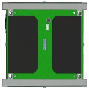
\includegraphics[height=7mm]{cube-icon}}};
}

%digram showing bias windows for the alignment algorithm

\begin{tikzpicture}


    \def\incline{90}                            % Orbit Inclination (degrees)
    \def\poleWindow{10}                         % Polar alignment windows in degrees
    \def\offset{10}                             % Amount the window is offset in the wake direction (i.e.  earlier) in degrees eq_window = 15;
    \def\eqWindow{15}                           % Equatorial alignment window in degrees
    %\def\latTrigger{\incline-\poleWindow}       % Corrects polar window for inclination angle
    \def\latTrigger{80}                         % Corrects polar window for inclination angle

    \def\winR{3cm}                                %window radius for drawing
    \def\axisLen{4cm}

    %import earth background
    \pgftext{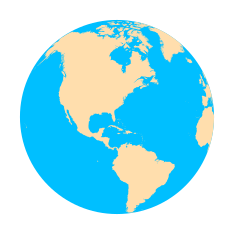
\includegraphics[height=4cm]{earth}}

    %draw orbit
    \draw[->,black,thin] (0,0) circle (\winR);

    %draw axis
    \draw[<->] (-\axisLen,0) -- (\axisLen,0);
    \draw[<->] (0,-\axisLen) -- (0,\axisLen);

    {
        \tikzset{>=triangle 45} %make a bigger arrow
        \draw[->] (25:\winR+0.5cm) arc (25:45:\winR+0.5cm);
        \draw[winLbl]   (35:\winR+0.5cm) node[anchor=south west] {\small Orbit Direction};
    }


    %draw bias windows
    %northbound equatorial window
    \draw[green]                    (0,0)  -- (\eqWindow/2 - \offset:\winR) arc (\eqWindow/2 - \offset:-\eqWindow/2 - \offset:\winR) -- cycle;
    \fill[nearly transparent,green] (0,0)  -- (\eqWindow/2 - \offset:\winR) arc (\eqWindow/2 - \offset:-\eqWindow/2 - \offset:\winR) -- cycle;

    \draw[green,winLbl] (-\offset:\winR+0.5cm) node[anchor=north west] {\small Northbound Equatorial Window};
    \cubesat{-\offset}{\winR}


    %south bound equatorial window
    \draw[red]                    (0,0)  -- (180-\eqWindow/2 - \offset:\winR) arc (180-\eqWindow/2 - \offset:180 +\eqWindow/2 - \offset:\winR) -- cycle;
    \fill[nearly transparent,red] (0,0)  -- (180-\eqWindow/2 - \offset:\winR) arc (180-\eqWindow/2 - \offset:180 +\eqWindow/2 - \offset:\winR) -- cycle;

    \draw[red,winLbl] (180-\offset:\winR+0.5cm) node[anchor=south east] {\small Southbound Equatorial Window};
    \cubesat{180-\offset}{\winR}


    %north polar window
    \draw[blue]                    (0,0)  -- (\latTrigger - \offset:\winR) arc (\latTrigger - \offset:90:\winR) -- cycle;
    \fill[nearly transparent,blue] (0,0)  -- (\latTrigger - \offset:\winR) arc (\latTrigger - \offset:90:\winR) -- cycle;

    \draw[blue,winLbl] (90-\poleWindow/2-\offset/2:\winR+0.5cm) node[anchor=south west] {\small North Polar Window};

    %draw CubeSat
    \cubesat{90-\poleWindow/2-\offset/2}{\winR}

    %draw axis labels
    \draw (0,\axisLen) node[anchor=south] {N};
    \draw (\axisLen,0) node[anchor=west] {E};

    \draw (0,-\axisLen) node[anchor=north] {S};
    \draw (-\axisLen,0) node[anchor=east] {W};

\end{tikzpicture}

    \caption{Bias windows for alignment mode}
    \label{fig:windows}
\end{figure}

\Cref{fig:windows} shows that the bias windows are offset so that they occur just before the equator or pole. The reason for this is shown in \cref{fig:winplace}. If the torquers are biased before the satellite passes over the vertical (or horizontal) field lines then the tendency is to rotate in the desired direction. If the torquers are biased afterwards then the tendency is to rotate the satellite in the opposite direction than is desired.\cite{Mentch11}

\begin{figure}[htb!]
    \centering
    \newcommand{\cubesat}[2]{
        \draw (#1:#2) node{\pgftext[rotate=#1]{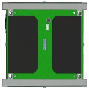
\includegraphics[height=15mm]{cube-icon}}};
        \draw[->,cyan,axis] (#1:#2) -- +(#1+90:\axlen);
        \draw (#1:#2) ++(#1+90:\axlen) node[rotate=#1-90,anchor=south west] {\tiny +Y};
        \draw[->,red,axis] (#1:#2) -- +(#1:\axlen);
        \draw (#1:#2) ++(#1:\axlen) node[rotate=#1-90,anchor=north west] {\tiny -Z};
    }

    \tikzstyle field=[color=blue,thick,postaction={decorate,decoration={markings,
        mark=at position .35 with {\arrowreversed[thin]{Latex[length=8mm,width=3mm,fill=red]}}}}]
    \tikzstyle axis=[thick]
    \tikzstyle motion=[very thick]
    
    \begin{tikzpicture}[>=stealth]
        \def\winR{4.5cm}                                %window radius for drawing
        \def\earthR{3.2cm}                              %earth radius for drawing
        \def\axlen{1.5cm}                               %axis length for drawing
        \def\favang{65}                                 %angle for favorable orientation
        \def\unfavang{115}                              %angle for unfavorable orientation
        \def\bias{35}                                   %half angle for bias arrows
        \begin{scope}
            %\clip (0,0) ellipse (6.3 and 3.5);
            \clip (-\winR,2cm) rectangle (\winR,\winR+\axlen);

            %draw vertical field line
            \draw[color=blue,field] (0,\earthR) -- (0,\winR+\axlen);
            %draw "earth"
            \draw[color=green!60!black,very thick] (0,0) circle (\earthR);

            %draw favorable cubesat
            \cubesat{\favang}{\winR}
            \draw[<->,YellowOrange,motion] (\favang:\winR+0.5cm) ++(\favang-\bias:0.5cm) arc (\favang-\bias:\favang+\bias:0.5cm);
            \draw[->,Plum,motion] (\favang:\winR+1cm) ++(\favang-90:0.7cm) arc (\favang-90:\favang+90:0.7cm);

            %draw unfavorable cubesat
            \cubesat{\unfavang}{\winR}
            \draw[<->,YellowOrange,motion] (\unfavang:\winR+0.5cm) ++(\unfavang-\bias:0.5cm) arc (\unfavang-\bias:\unfavang+\bias:0.5cm);
            \draw[<-,Plum,motion] (\unfavang:\winR+1cm) ++(\unfavang-90:0.7cm) arc (\unfavang-90:\unfavang+90:0.7cm);

        \end{scope}
        \draw (\unfavang:\winR) ++(\unfavang:\axlen+0.2cm) node[rotate=\unfavang-90,anchor=south] {\tiny Unfavorable};
        \draw (\favang:\winR) ++(\favang:\axlen+0.2cm) node[rotate=\favang-90,anchor=south] {\tiny Favorable};
    \end{tikzpicture}
    \caption{Bias window offset}
    \label{fig:winplace}
\end{figure}

\subsection{Mode 2}

Mode 2 is initiated at the end of the detumble phase. In mode 2 the torquers are biased as shown in \cref{fig:m2b} and while the bias is active the algorithm in \cref{eqn:crossl} is used to dampen out the oscillations caused by the bias. Outside the three bias windows all torquers are set to cancel each other and the \ac{ARC} coasts.

\begin{figure}[htb!]
    \centering
    \newcommand{\cubesat}[2]{
        \draw (#1:#2) node{\pgftext[rotate=#1]{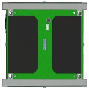
\includegraphics[height=9mm]{cube-icon}}};
        \draw[->,cyan,axis] (#1:#2) -- +(#1+90:\axlen);
        \draw (#1:#2) ++(#1+90:\axlen) node[rotate=#1-90,anchor=south] {\tiny +Y};
        \draw[->,red,axis] (#1:#2) -- +(#1:\axlen);
        \draw (#1:#2) ++(#1:\axlen) node[rotate=#1-90,anchor=west] {\tiny -Z};
    }

    \tikzstyle field=[arrows={-Latex[color=blue,fill=red,length=3mm,width=1.5mm]}]
    \tikzstyle axis=[thick]
    \tikzstyle motion=[YellowOrange,very thick]
    
    \begin{tikzpicture}[>=stealth]
        \def\winR{2.4cm}                                %window radius for drawing
        \def\earthR{1.8cm}                              %earth radius for drawing
        \def\axlen{1cm}                                 %axis length for drawing
        \def\favang{65}                                 %angle for favorable orientation
        \def\unfavang{115}                              %angle for unfavorable orientation
        \def\bias{35}                                   %half angle for bias arrows
        \begin{scope}6511478
            \clip (0,0) circle (3cm);
            %\clip (0,0) circle (8.5);

            %draw "earth"
            \draw[color=green!60!black,thick] (0,0) circle (\earthR);

            % Computes a point on a field line given r and t
            \newcommand{\fieldlinecurve}[2]{%
                {(pow(#1,2))*(3*cos(#2)+cos(3*(#2)))*0.7}, {(pow(#1,2))*(sin(#2)+sin(3*(#2)))}%
            }

            \foreach \r in {0.85,0.98,1.3,1.8} {
                \draw[color=blue,smooth,variable=\t, samples at={0,-5,-10,...,-360}] plot (\fieldlinecurve{\r}{\t});
            }

            \draw[field] (\fieldlinecurve{0.85}{17}) -- (\fieldlinecurve{0.85}{23});
            \draw[field] (\fieldlinecurve{0.98}{23}) -- (\fieldlinecurve{0.98}{28});
            \draw[field] (\fieldlinecurve{1.3}{50}) -- (\fieldlinecurve{1.3}{52});
            \draw[field] (\fieldlinecurve{1.8}{65}) -- (\fieldlinecurve{1.8}{65.5});

            \draw[field] (\fieldlinecurve{0.85}{-23}) -- (\fieldlinecurve{0.85}{-17});
            \draw[field] (\fieldlinecurve{0.98}{-28}) -- (\fieldlinecurve{0.98}{-23});
            \draw[field] (\fieldlinecurve{1.3}{-52}) -- (\fieldlinecurve{1.3}{-50});
            \draw[field] (\fieldlinecurve{1.8}{-65.5}) -- (\fieldlinecurve{1.8}{-65});

            \draw[field] (\fieldlinecurve{0.85}{180-17}) -- (\fieldlinecurve{0.85}{180-23});
            \draw[field] (\fieldlinecurve{0.98}{180-23}) -- (\fieldlinecurve{0.98}{180-28});
            \draw[field] (\fieldlinecurve{1.3}{180-50}) -- (\fieldlinecurve{1.3}{180-52});
            \draw[field] (\fieldlinecurve{1.8}{180-65}) -- (\fieldlinecurve{1.8}{180-65.5});

            \draw[field] (\fieldlinecurve{0.85}{180+23}) -- (\fieldlinecurve{0.85}{180+17});
            \draw[field] (\fieldlinecurve{0.98}{180+28}) -- (\fieldlinecurve{0.98}{180+23});
            \draw[field] (\fieldlinecurve{1.3}{180+52}) -- (\fieldlinecurve{1.3}{180+50});
            \draw[field] (\fieldlinecurve{1.8}{180+65.5}) -- (\fieldlinecurve{1.8}{180+65});
        \end{scope}

        %draw cubesat in windows
        \cubesat{90}{\winR}
        \draw[<->,motion] (90:\winR) ++(90:0.1cm) ++(90-\bias:0.5cm) arc (90-\bias:90+\bias:0.5cm);
        \cubesat{180}{\winR}
        \draw[<->,motion] (180:\winR) ++(-90:0.1cm) ++(90+180-\bias:0.5cm) arc (90+180-\bias:90+180+\bias:0.5cm);
        \cubesat{0}{\winR}
        \draw[<->,motion] (0:\winR) ++(90:0.1cm) ++(90-\bias:0.5cm) arc (90-\bias:90+\bias:0.5cm);

        %draw magnet
        \fill[color=white] (0.25,0.5) rectangle (-0.25,0);
        \fill[color=red] (0.25,0) rectangle (-0.25,-0.5);
        \draw[color=red] (0, 0.2) node {S};
        \draw[color=white] (0,-0.2) node {N};
        \draw[color=black] (0.25,0.5) rectangle (-0.25,-0.5);
    \end{tikzpicture}
    \caption{Bias regions for mode 2}
    \label{fig:m2b}
\end{figure}

The purpose of mode 2 is to get the satellite, which is in a random orientation, into the desired orientation. The original simulation transitioned from mode 2 to mode 3 after a fixed 10 orbits. This was shown to get the satellite into the desired orientation.

\subsection{Mode 3}

Mode 3 is initiated after mode 2 is complete. In mode 3 only the north pole bias window is used as shown in \cref{fig:m3b}. Outside the bias window however the algorithm in \cref{eqn:crossl} is used to maintain desired rotation rates.

\begin{figure}[htb!]
    \centering
    \newcommand{\cubesat}[2]{
        \draw (#1:#2) node{\pgftext[rotate=#1]{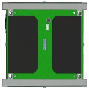
\includegraphics[height=9mm]{cube-icon}}};
        \draw[->,cyan,axis] (#1:#2) -- +(#1+90:\axlen);
        \draw (#1:#2) ++(#1+90:\axlen) node[rotate=#1-90,anchor=south] {\tiny +Y};
        \draw[->,red,axis] (#1:#2) -- +(#1:\axlen);
        \draw (#1:#2) ++(#1:\axlen) node[rotate=#1-90,anchor=west] {\tiny -Z};
    }

    \tikzstyle field=[arrows={-Latex[color=blue,fill=red,length=3mm,width=1.5mm]}]
    \tikzstyle axis=[thick]
    \tikzstyle motion=[YellowOrange,very thick]
    
    \begin{tikzpicture}[>=stealth]
        \def\winR{2.4cm}                                %window radius for drawing
        \def\earthR{1.8cm}                              %earth radius for drawing
        \def\axlen{1cm}                                 %axis length for drawing
        \def\favang{65}                                 %angle for favorable orientation
        \def\unfavang{115}                              %angle for unfavorable orientation
        \def\bias{35}                                   %half angle for bias arrows
        \begin{scope}6511478
            \clip (0,0) circle (3cm);
            %\clip (0,0) circle (8.5);

            %draw "earth"
            \draw[color=green!60!black,thick] (0,0) circle (\earthR);

            % Computes a point on a field line given r and t
            \newcommand{\fieldlinecurve}[2]{%
                {(pow(#1,2))*(3*cos(#2)+cos(3*(#2)))*0.7}, {(pow(#1,2))*(sin(#2)+sin(3*(#2)))}%
            }

            \foreach \r in {0.85,0.98,1.3,1.8} {
                \draw[color=blue,smooth,variable=\t, samples at={0,-5,-10,...,-360}] plot (\fieldlinecurve{\r}{\t});
            }

            \draw[field] (\fieldlinecurve{0.85}{17}) -- (\fieldlinecurve{0.85}{23});
            \draw[field] (\fieldlinecurve{0.98}{23}) -- (\fieldlinecurve{0.98}{28});
            \draw[field] (\fieldlinecurve{1.3}{50}) -- (\fieldlinecurve{1.3}{52});
            \draw[field] (\fieldlinecurve{1.8}{65}) -- (\fieldlinecurve{1.8}{65.5});

            \draw[field] (\fieldlinecurve{0.85}{-23}) -- (\fieldlinecurve{0.85}{-17});
            \draw[field] (\fieldlinecurve{0.98}{-28}) -- (\fieldlinecurve{0.98}{-23});
            \draw[field] (\fieldlinecurve{1.3}{-52}) -- (\fieldlinecurve{1.3}{-50});
            \draw[field] (\fieldlinecurve{1.8}{-65.5}) -- (\fieldlinecurve{1.8}{-65});

            \draw[field] (\fieldlinecurve{0.85}{180-17}) -- (\fieldlinecurve{0.85}{180-23});
            \draw[field] (\fieldlinecurve{0.98}{180-23}) -- (\fieldlinecurve{0.98}{180-28});
            \draw[field] (\fieldlinecurve{1.3}{180-50}) -- (\fieldlinecurve{1.3}{180-52});
            \draw[field] (\fieldlinecurve{1.8}{180-65}) -- (\fieldlinecurve{1.8}{180-65.5});

            \draw[field] (\fieldlinecurve{0.85}{180+23}) -- (\fieldlinecurve{0.85}{180+17});
            \draw[field] (\fieldlinecurve{0.98}{180+28}) -- (\fieldlinecurve{0.98}{180+23});
            \draw[field] (\fieldlinecurve{1.3}{180+52}) -- (\fieldlinecurve{1.3}{180+50});
            \draw[field] (\fieldlinecurve{1.8}{180+65.5}) -- (\fieldlinecurve{1.8}{180+65});
        \end{scope}

        %draw cubesat in windows
        \cubesat{90}{\winR}
        \draw[<->,motion] (90:\winR) ++(90:0.1cm) ++(90-\bias:0.5cm) arc (90-\bias:90+\bias:0.5cm);

        %draw magnet
        \fill[color=white] (0.25,0.5) rectangle (-0.25,0);
        \fill[color=red] (0.25,0) rectangle (-0.25,-0.5);
        \draw[color=red] (0, 0.2) node {S};
        \draw[color=white] (0,-0.2) node {N};
        \draw[color=black] (0.25,0.5) rectangle (-0.25,-0.5);
    \end{tikzpicture}
    \caption{Bias region for mode 3}
    \label{fig:m3b}
\end{figure}

\section{Simulation Results}

The simulations in \cite{Mentch11} showed that tipoff rates of 5\textdegree/sec could be arrested within two 98\textdegree{} inclination orbits. In mode 3 the simulations showed that the desired orientation was achieved within 2\textdegree{} in all axes using alnico1 torquers for detumble and vernier torquers for alignment.


\section{Concept of Operations for the \acl{ARC}}

The initial concept was proposed by Mentch in \cite{Mentch11}. The concept was largely based on what was possible in simulation. The simulation allowed the satellite perfect knowledge of the rotation rates which are not trivial to calculate from the magnetic field as suggested. The rotation rates can be calculated from the magnetic field using a Kalman filter as suggested in \cite{Sturm05} but this is beyond the scope of this thesis.

Difficulties were also encountered with the torquers. The vernier torquers were proposed to be $\sfrac{1}{200}$ the size of the primary torquers. This presented two problems: manufacturing and balancing. Finding a suitable, weaker, magnetic material for the torquers proved difficult as Mentch said ``There isn't much of a marked for crappy magnets.'' The solution that was proposed was to coat a non magnetic rod with a very thin layer of magnetic material using a vacuum deposition process. There were difficulties getting torquers and later tests showed that there is enough variation in the dipole moment of the primary torquers to overwhelm the vernier torquers. 

Because of these difficulties the \ac{ACDS} was re-scoped to focus on detumble. Instead of one pair of primary torquers and one pair of vernier torquers two pairs of primary torquers are used. This gives four possible states as shown in \cref{fig:lpmtq-flt}.

\begin{figure}[H]
    \centering
    \begin{tikzpicture}
    \def\L{1.5}     %define arrow length
    \draw[->,red,very thick] ( 0.25, 0) -- ( 0.25,\L);
    \draw[->,red,very thick] ( 0.75, 0) -- ( 0.75,\L);
    \draw[->,red,very thick] ( 1.25, 0) -- ( 1.25,\L);
    \draw[->,red,very thick] ( 1.75, 0) -- ( 1.75,\L);
    \draw (1 ,-0.5) node {+4M};

    \draw[->,red,very thick] (3.25,\L) -- ( 3.25, 0);
    \draw[->,red,very thick] (3.75, 0) -- ( 3.75,\L);
    \draw[->,red,very thick] (4.25, 0) -- ( 4.25,\L);
    \draw[->,red,very thick] (4.75, 0) -- ( 4.75,\L);
    \draw (4 ,-0.5) node {+2M};

    \draw[->,red,very thick] ( 6.25,\L) -- ( 6.25, 0);
    \draw[->,red,very thick] ( 6.75,\L) -- ( 6.75, 0);
    \draw[->,red,very thick] ( 7.25, 0) -- ( 7.25,\L);
    \draw[->,red,very thick] ( 7.75, 0) -- ( 7.75,\L);
    \draw (7 ,-0.5) node {0M};

    \draw[->,red,very thick] ( 9.25,\L) -- ( 9.25, 0);
    \draw[->,red,very thick] ( 9.75,\L) -- ( 9.75, 0);
    \draw[->,red,very thick] (10.25,\L) -- (10.25, 0);
    \draw[->,red,very thick] (10.75, 0) -- (10.75,\L);
    \draw (10,-0.5) node {-2M};

    \draw[->,red,very thick] (12.25,\L) -- (12.25, 0);
    \draw[->,red,very thick] (12.75,\L) -- (12.75, 0);
    \draw[->,red,very thick] (13.25,\L) -- (13.25, 0);
    \draw[->,red,very thick] (13.75,\L) -- (13.75, 0);
    \draw (13,-0.5) node {-4M};
    \end{tikzpicture}
    \caption{Possible dipole moments for two torquer pairs}
    \label{fig:moments-flt}
\end{figure}

Because there are more torquer states the quantization function shown in \cref{fig:lpmtq} is changed to \cref{fig:lpmtq-flt}. The increased number of torquers increases the maximum torque but doesn't change the minimum possible torque.

\begin{figure}[htb!]
    \centering
    \begin{tikzpicture}

 
    \draw[<->,green,very thick] (4,4) -- (3,4) -- (3,2) -- (1,2) -- (1,0) -- (-1,0) -- (-1,-2) -- (-3,-2) -- (-3,-4) -- (-4,-4);
 
    %draw axis
    \draw[<->] (-5,0) -- (5,0);
    \draw[<->] (0,-5) -- (0,5);
 
    %draw axis labels
    \draw (0,5) node[anchor=south] {$m_{command_q}$};
    \draw (5,0) node[anchor=west] {$m_{command}$};

    \draw (4,0)  node[anchor=north] {$+4M$};
    \draw (3,0)  node[anchor=north] {$+3M$};
    \draw (2,0)  node[anchor=north] {$+2M$};
    \draw (1,0)  node[anchor=north] {$+1M$};
    \draw (-1,0) node[anchor=south] {$-1M$};
    \draw (-2,0) node[anchor=south] {$-2M$};
    \draw (-3,0) node[anchor=south] {$-3M$};
    \draw (-4,0) node[anchor=south] {$-4M$};

    \draw (0,4)  node[anchor=east] {$+4M$};
    \draw (0,2)  node[anchor=east] {$+2M$};
    \draw (0,-2) node[anchor=west] {$-2M$};
    \draw (0,-4) node[anchor=west] {$-4M$};

    \end{tikzpicture}
    \caption{Quantization function for flight \acsp{LPMT}}
    \label{fig:lpmtq-flt}
\end{figure}

Adding a second set of primary torquers allows a larger dipole moment during the detumble phase but does not help during the alignment phase when smaller torques need to be generated. The original design used a 10~second charge time which meant that once a torquer was flipped it would be torquing the satellite for a minimum 10~seconds. To help mitigate the use of more powerful torquers the charge time was changed to 1~second. This means that the minimum time that the torquers can be torquing is reduced, reducing the overall change in angular velocity of the satellite. The reduction in charge time is only by a factor of 10 but the minimum torque was increased by a factor of 200 so the pointing accuracy of the satellite will suffer.

Rotation rate determination also proved a challenge for the on orbit implementation. The satellite in simulation had full knowledge of the rotation rates. In \cite{Mentch11} it was proposed that rotation rates could be directly calculated using the magnetic field. 

Using the magnetic field to determine rotation rates does not give the full rotation rate vector. Instead the rotation rate vector is in effect projected onto the magnetic field, eliminating any rotation rate around the magnetic field. Originally it was believed that this would not be a problem because the torquers can't be used to stop rotation around the magnetic field. Simulations showed, however, that when the rotation rate vector was projected onto the magnetic field then the attitude control did not work.

The other problem with rate determination is that the desired rotation of the satellite is to rotate once every orbit in one axis an no rotation in the other axes. The expected orbital period is about 90~minutes so this gives a rotation rate of 0.011~rpm or 1.16~mrad/sec. In 10~seconds a satellite rotating at this rate will rotate about 20~\textmu\textdegree. For a satellite rotating in a 300~mGauss magnetic field this results in a 60~\textmu Gauss field change every 10 seconds. Thus in order to measure the rotation rates of the satellite the magnetic field of the earth must be measured with an accuracy that is on the order of 10s of \textmu Gauss. 

In \cite{Sturm05} a Kalman filter is used to calculate rotation rates from magnetic field measurements. This solution solves both problems. By taking into account the spacecraft dynamics, the full rotation rate vector can be estimated. Because the rates come from the estimated system state they are less noisy than those from a single set of magnetic field measurements. The problem is that Kalman filters are not trivial to get working and must correctly model the system to function correctly. This is beyond the scope of this thesis so the alignment phase of the attitude control system is not implemented.

\subsection{B-dot control}

Because of the lack of a Kalman filter for the flight implementation the algorithm in \cref{eq:crossl} can not be used. To detumble the satellite without rotation rates the B-dot algorithm is used. This uses the time derivative of of the magnetic field instead of calculating the rotation rates.

\begin{equation}
    \vec{m}_{command}= C \dot{\vec{B}}
    \label{eq:bg-bdot}
\end{equation}

\Cref{eq:bg-bdot} shows the B-dot control law. Because $\dot{\vec{B}}$ results largely from the spacecraft rotation, it is largely perpendicular to $\vec{B}$. This results in a dipole moment that is perpendicular to the magnetic field which is desirable for efficiency reasons. The gain $C$ is a scalar value less than zero that is used to tune the algorithm. Large values of $C$ increase the sensitivity of the algorithm and allow it to detumble to a lower rotation rate. Lower values of $C$ are less sensitive to noise.

\begin{comment}
\subsection{Detumble}

The goal of the detumble mode is to reduce the rotation rates down to an acceptable level \todo{possibly call out such a level}.

%\subsubsection{upload orbital information}

%To correctly calculate attitude and rotation rates orbital parameters must be uplinked. Before this happens detumble can not complete. Once the orbital parameters are uplinked the Kalman filter will likely have to re-adjust which may necessitate that detumble stop for a short period. Once the filter has re-adjusted detumble will still likely have to run for a bit to get the rates within tolerances.

\subsection{Alignment}

Once detumble is complete the alignment procedure begins. The alignment procedure takes a fixed 12 \todo{Double check this number} orbits to complete.

\subsubsection{Attitude Determination}

The original design did not use attitude determination to get the satellite into the proper orientation. Instead the rotation rates are used along with the bias windows to get the satellite into the right alignment. The problem is that computing the rotation to the needed accuracy is not a simple process. The original idea was that the rotation rates could be computed directly from magnetic field measurements. A set of magnetometer measurements would be taken each time step to compute the rotation rates. The problem is that to do the rotation rate calculation a derivative is needed. Numerical differentiation is possible but it tends to increase noise by acting as a high pass filter.

The proposed rate determination algorithm also falls short because it does not estimate the full rotation rates. Because the magnetic field is used to determine rotation rates rotations around the magnetic field can not be resolved. This was thought not to be an issue because these rotations are also the kind that can not be corrected for by the torquers but it was shown,in simulation, that removing the component of the rotation rates parallel to the magnetic field caused the CubeSat not to stabilize into the proper alignment. 

To solve both of these problems a Kalman filter is used to estimate both the attitude and the rotation rates using the magnetic field data. The Kalman filter estimates the rates by using the assumed satellite dynamics along with a magnetic field model. The Kalman filter uses the knowledge of the system dynamics to smooth the rate estimates and reduce noise. 



\begin{equation}
    F_k = 
        \begin{bmatrix}
              0                &   \hat {\omega} _3 & - \hat {\omega} _2  & \frac{1}{2} & 0           & 0           \\
            - \hat {\omega} _3 &   0                &   \hat {\omega} _1  & 0           & \frac{1}{2} & 0           \\
              \hat {\omega} _2 & - \hat {\omega} _1 &   0                 & 0           & 0           & \frac{1}{2} \\
            0 & 0 & 0 & 0                  & K_1 \hat{\omega}_3 & K_1 \hat{\omega}_2 \\
            0 & 0 & 0 & K_2 \hat{\omega}_3 & 0                  & K_2 \hat{\omega}_1 \\
            0 & 0 & 0 & K_3 \hat{\omega}_2 & K_3 \hat{\omega}_1 & 0                  \\
        \end{bmatrix}
\end{equation}

\begin{equation}
    \Phi \left( t \right) = \matt{I} + \matt{F} t = 
        \begin{bmatrix}
              1                  &   \hat {\omega} _3 t & - \hat {\omega} _2 t  & \frac{1}{2} t & 0             & 0             \\
            - \hat {\omega} _3 t &   1                  &   \hat {\omega} _1 t  & 0             & \frac{1}{2} t & 0             \\
              \hat {\omega} _2 t & - \hat {\omega} _1 t &   1                   & 0             & 0             & \frac{1}{2} t \\
            0 & 0 & 0 & 1                    & K_1 \hat{\omega}_3 t & K_1 \hat{\omega}_2 t \\
            0 & 0 & 0 & K_2 \hat{\omega}_3 t & 1                    & K_2 \hat{\omega}_1 t \\
            0 & 0 & 0 & K_3 \hat{\omega}_2 t & K_3 \hat{\omega}_1 t & 1                    \\
        \end{bmatrix}
\end{equation}

\begin{equation}
    \matt{Q} = Q \matt{I}
\end{equation}

\begin{equation}
    \matt{Q}_k = \int _0 ^ {T_s} \matt{\Phi} \left( \tau \right) \matt{Q} \matt{\Phi} \transpose \left( \tau \right) d\tau = Q \int _0 ^ {T_s} \matt{\Phi} \left( \tau \right) \matt{\Phi} \transpose \left( \tau \right) d\tau
\end{equation}


\begin{equation}
    \matt{Q}_k = Q \int _0 ^ {T_s} \matt{\Phi} \left( \tau \right) \matt{\Phi} \transpose \left( \tau \right) d\tau
\end{equation}

\subsection{Operations Mode}

Once alignment is complete the \ac{ACDS} transitions into operations mode. In operations mode the \ac{ACDS} maintains alignment with the desired attitude.

\subsubsection{detect/correct alternate stable configurations}

In operations mode the \ac{ACDS} will check to see if \ac{ARC} has settled into an alternate stable configurations and correct for such conditions. If a correction is made the \ac{ACDS} drops back to alignment mode after the correction is complete.

\subsection{Contingency}

Because the \ac{ACDS} is an experimental system there is a high likelihood that things will go wrong. To account for this the software is written in a way that allows the operation to be changed in case of poor performance. All the Kalman filter parameters and attitude control parameters will be changeable via ground station command.

\end{comment}


%% vim: set filetype=tex spell :

\chapter{CubeSat Implementation}

\label{ch:CubeSat}

%ConOps to background

%Tweak wording so kalman filter comes later

%Also move contingency later

%.1 Torquers
%crank said what he wanted. I say what we can have. Talk about firing circuits.
%.2 Measurements
%present analysis of expected accuracy. Requirement to determination rotation rate. Talk about instrumentation to get there. (Kalman optional)

The block diagram for the CubeSat hardware used to implement the \ac{ADCS}. The hardware necessary for the \ac{ADCS} is spread over multiple subsystems of the \ac{ARC}. The \ac{ADCS} board contains the torquers, driving hardware along with the microcontroller which will run the algorithm. There is one two axis magnetometer located on each of the six of the \acp{SPB}. These are used by the \ac{ADCS} to calculate rotation rates and calculate the magnetic dipole moment required to generate the necessary torque. Spreading the magnetometers across all six faces should give some degree of noise immunity and redundancy. The \ac{LEDL} board also contains \ac{MEMS} angular rate sensors as a redundant reading of the rotation rate of the \ac{ARC}. The sensors on the \acp{SPB} are read by the \ac{LEDL} which then forwards the magnetometer and angular rate measurements to the \ac{ADCS}.

\begin{figure}[H]
    \centering
    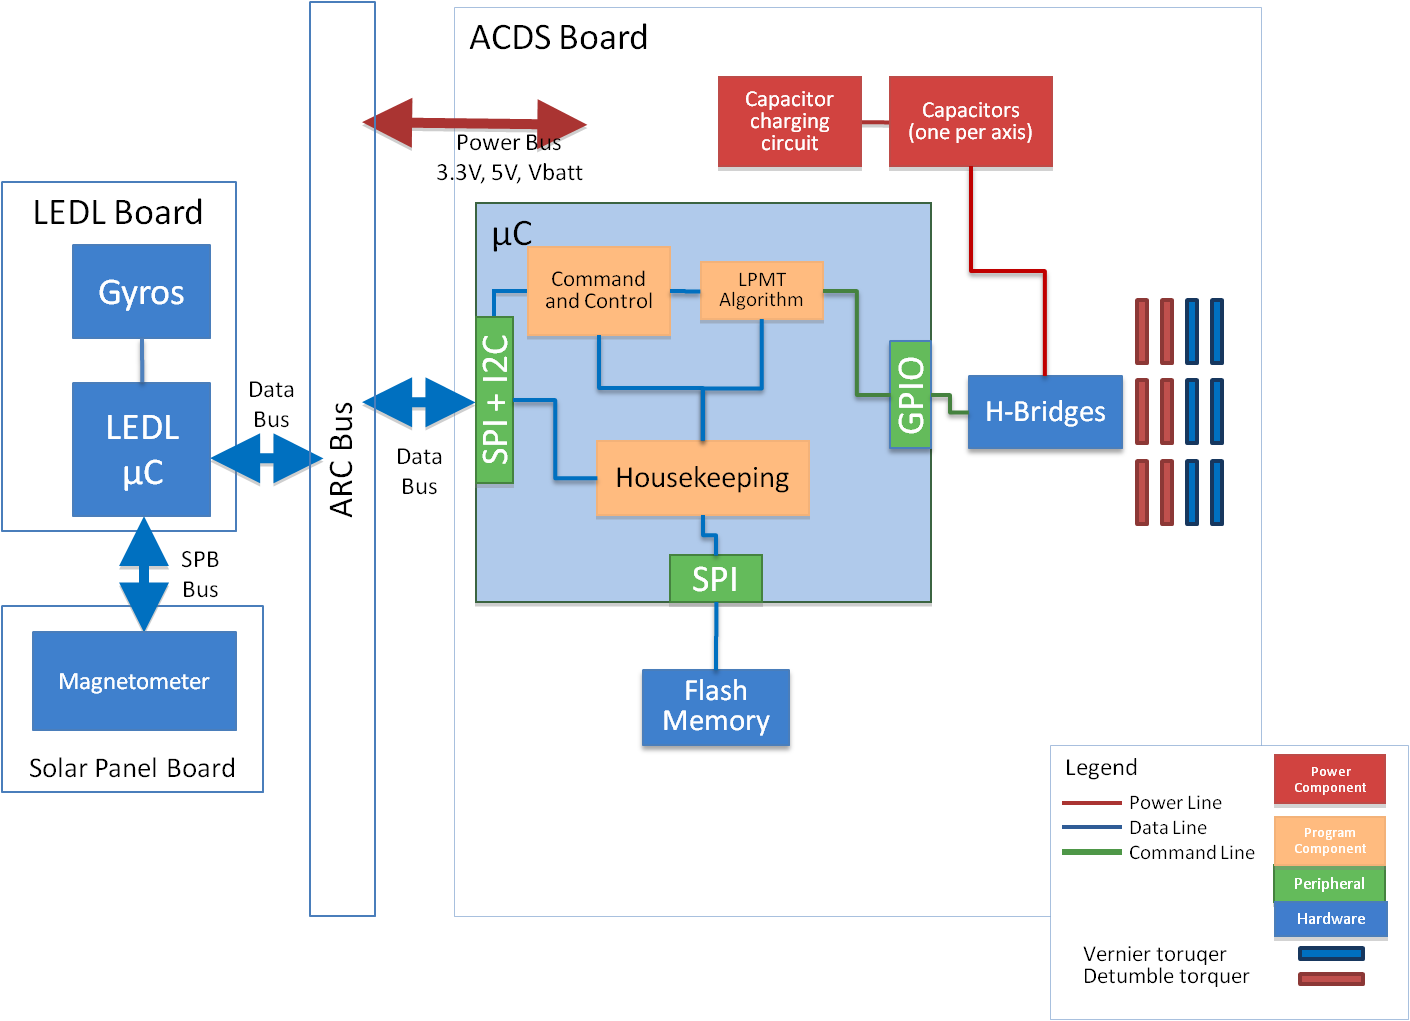
\includegraphics[width=0.8\textwidth]{Figures/Block}
    \caption{Block Diagram of the CubeSat \acs{ADCS} system}
\end{figure}

\section{Bus Communication}

The subsystems of the \ac{ARC} will communicate with each other using the ARCBus. The ARCBus consists of shared connections between the subsystems to transmit commands and data. The ARCBus will primary used by the \ac{ADCS} to get sensor data from the \ac{LEDL} and send and receive data to the ground station through the COMM system.

\section{Hardware}

\subsection{CubeSat Overview}

\begin{figure}[H]
    \centering
    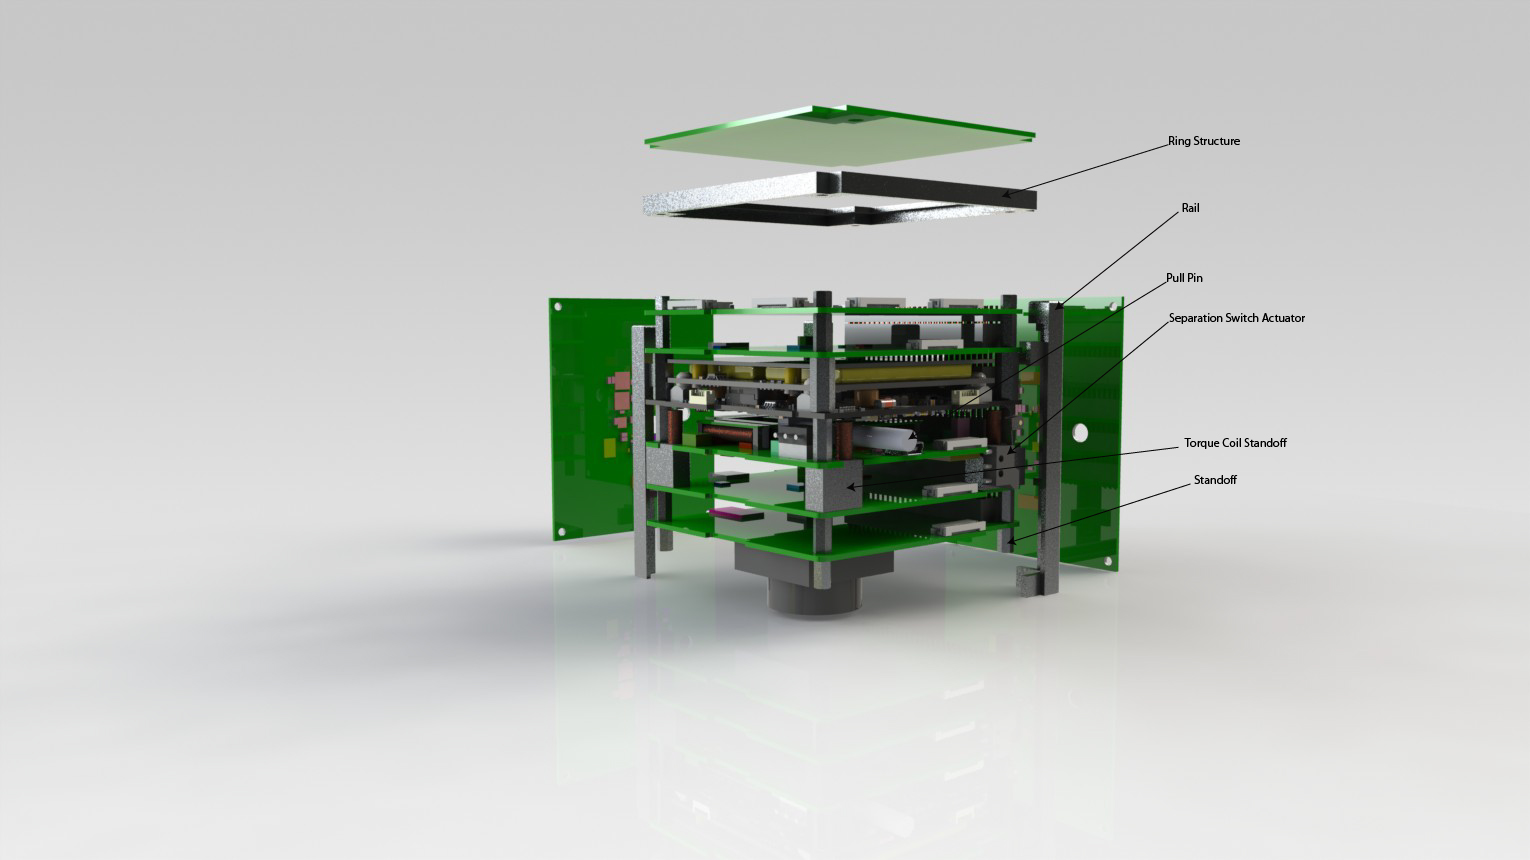
\includegraphics[width=0.8\textwidth]{Figures/CubeSat-Diagram}
    \caption{Diagram of the \ac{ARC}}
\end{figure}

\begin{figure}[H]
    \centering
    \includegraphics[width=0.8\textwidth]{Figures/cubesat-core}
    \caption{Core Board Stack of the \ac{ARC}}
\end{figure}

\subsection{Torquers}

\subsubsection{Cores}

The torquer cores from \cite{Mentch11} consisted of a large and a small pair in each axis. The torquers consist of a hard magnetic core an electromagnetic coil to flip the core. All torquer cores were the same size, one inch long $\sfrac{1}{16}$th inch diameter rod. The large pair was made of Alnico1 and produced a magnetic dipole moment of $0.022 \unit{A m^2}$. The small pair was proposed to have an inert core with a thin permalloy coating to give it a dipole moment of $0.00011 \unit{A m^2}$.

The torque that the alnico torquers produce is quite small and is already not easy to measure. Because the small torquers are $\sfrac{1}{200}$th the size of the alnico torquers it was determined that these are not feasible to fabricate. To fix this the small torquers was enlarged to 10\% of the size of the large torquers. The switching interval was also reduced to one second. It was also necessary to relax the desired attitude tolerances to accommodate the new setup.

\subsubsection{Drivers}

The schematic to drive a pair of torquers is shown in \autoref{fig:drive}. Each pair of torquers is driven by three complimentary pairs of \acp{MOSFET}.  The \acp{MOSFET} are driven by three pairs of \ac{MOSFET} drivers which are controlled by the \ac{ADCS} microcontroller.

In the idle state all of the \acp{MOSFET} are off and the torquer coils are floating. This prevents changing magnetic fields in the torquers causing current to flow in them. To flip a torquer one end of the torquer is shorted to ground using one of the N-Channel \acp{MOSFET} and the other end is shorted to C1 using one of the P-Channel \acp{MOSFET}. After a short delay the \acp{MOSFET} are switched off and C1 begins to recharge.

\begin{figure}[H]
    \centering
    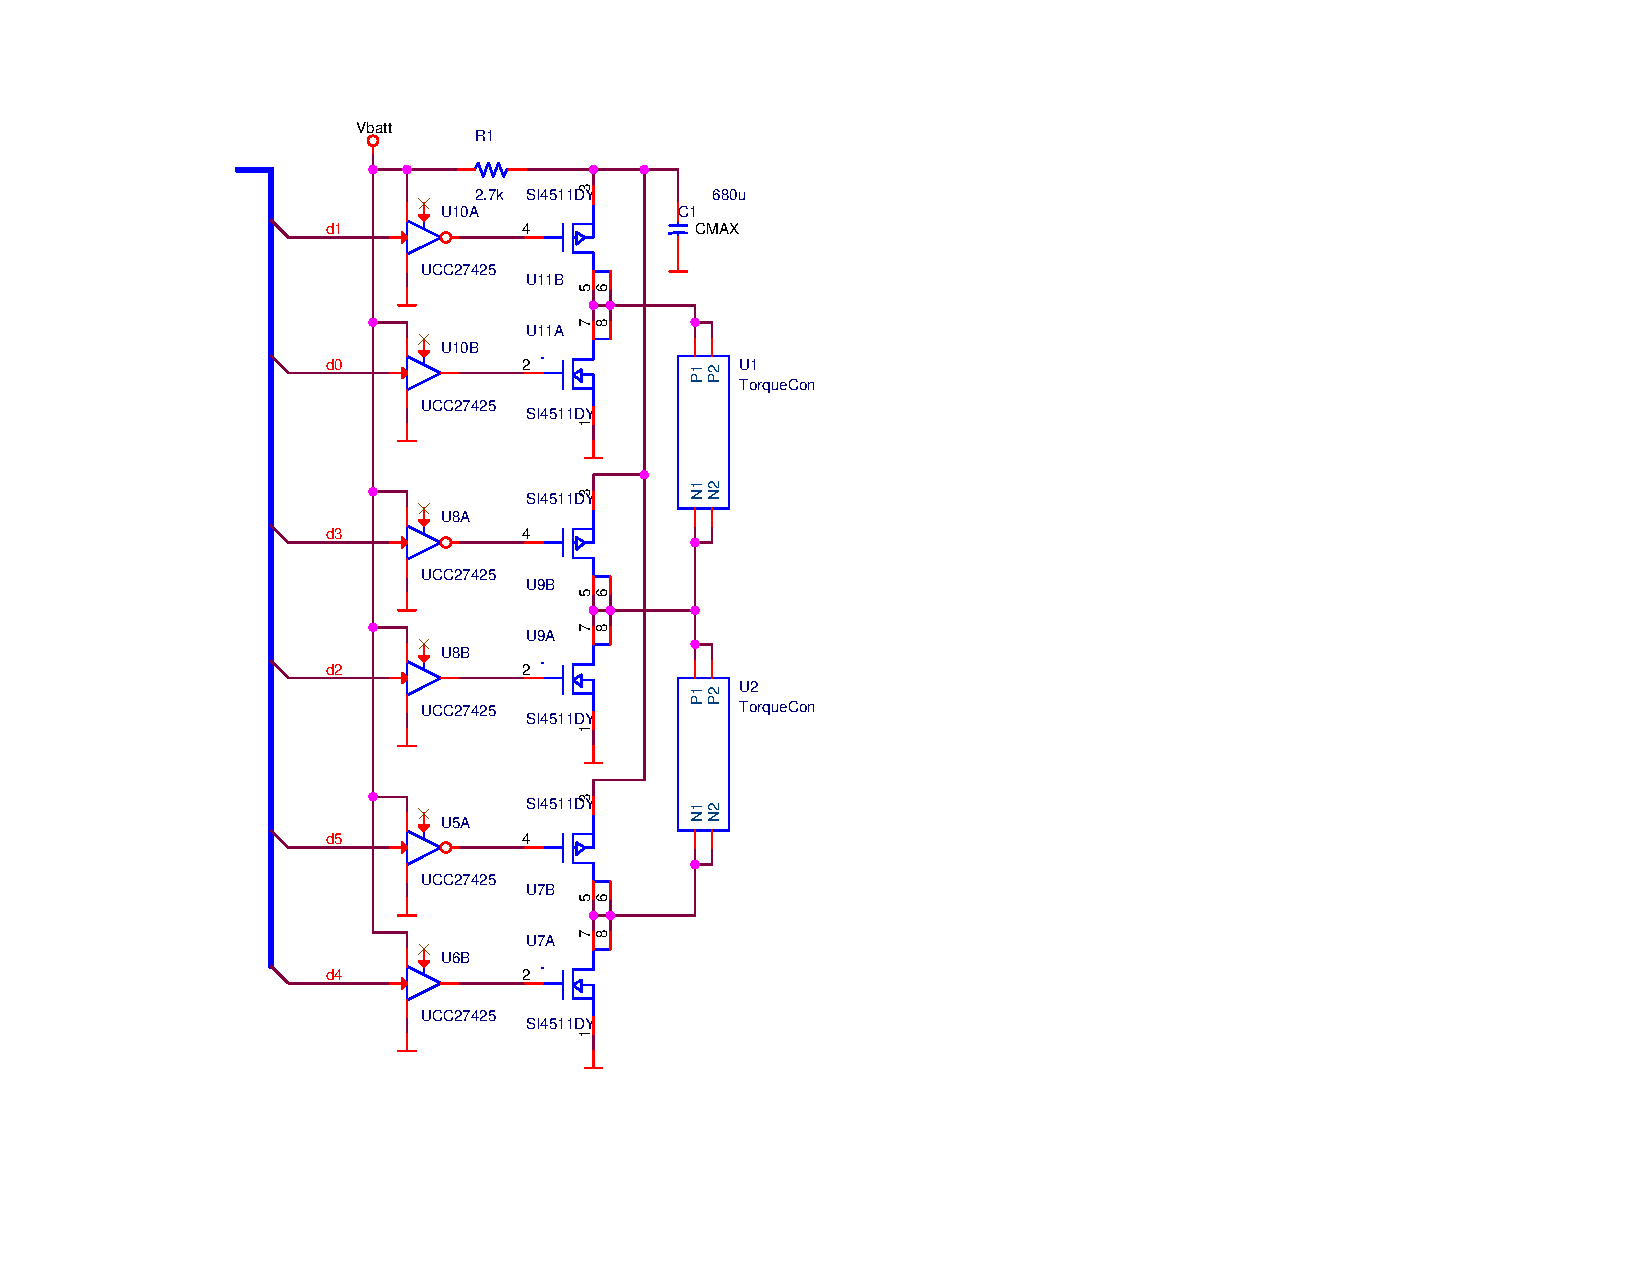
\includegraphics[width=0.5\textwidth]{Figures/driverSchematic}
    \caption{Torquer Driver schematic}
    \label{fig:drive}
\end{figure}

\subsection{Sensors}

The only sensor called out in \cite{Mentch11} was a magnetometer. The accuracy of the magnetometer was not specified but it needs to be able to determine rotation rates accurately enough for the \ac{ADCS} to work.

\subsubsection{Magnetometer}

The magnetometers on the satellite are Honeywell HMC1052 \ac{AMR} sensors. These sensors use \ac{AMR} elements in a bridge configuration to measure the field in each axis. The HMC1052 is a 2-axis sensor that measures the field in the axis that are parallel to the board that it is mounted on (X and Y). Each face of \ac{ARC} will have a single HMC1052 giving a total of 4 measurements in each axis.

The \ac{AMR} sensors are primarily sensitive to magnetic fields in their sensitive direction but they are also slightly sensitive to magnetic fields in an axis normal to the sensitive direction. The sensor is only sensitive to magnetic fields that are in the film plane, which is the plane that the \ac{AMR} film is deposited in. For the 2-axis HMC1052 this means that both sensors show some sensitivity to fields in both the X and Y axes. The cross axis effect varies from sensor to sensor \todo{Test this} so calibration values must be calculated for each sensor \cite{AN215}.

\autoref{eq:magfull} shows the full equation for the magnetometer. $V_b$ is the bridge voltage that is applied to the sensor. $S_s$ is the sensitivity in the sensitive direction. C and D are the cross field sensitivity and offset values \cite{AN215}.

\begin{equation}
    V_o = V_b \left( \left( S_s \left( 1 + C \cdot H_c^2 \right) H_s \right) + D \cdot H_c \right)
    \label{eq:magfull}
\end{equation}

Because C is small and is multiplied by miligauss squared to get a really small number, it is ignored for the purposes of calibration which results in the simpler \autoref{eq:magcross}.

\begin{equation}
    V_o = V_b \left( \left( S_s H_s \right) + D \cdot H_c \right)
    \label{eq:magcross}
\end{equation}

\autoref{eq:magcross} is useful to determine the voltage that would be produced for a given magnetic field condition, but not terribly useful if the sensor voltages are known but the fields are not. Furthermore the \ac{ADC} reference voltage will be the same as $V_b$ so knowing the bridge voltage is unnecessary\todo[prepend, caption={Elaborate Here?}]{Seems more or less obvious to me and somewhat cumbersome to fully explain}. 
 
\begin{equation}
    H = C_1 \cdot V_x + C_2 \cdot V_y + C_3
    \label{eq:magcal}
\end{equation}

Because $S_s$ and D from \autoref{eq:magcross} are experimentally determined, it is easier to solve \autoref{eq:magcross} for calibration instead. In this case $V_x$ and $V_y$ are the \ac{ADC} values for the x and y axis respectively. $C_1$ and $C_2$ are the sensitivity and $C_3$ is an offset that can come from offsets in the instrumentation or from external offsets such as torquers. This makes the values that the calibration solves for directly usable to calculate magnetic field from \ac{ADC} measurements.

\subsubsection{Magnetometer Calibration}

Magnetometer Calibration consists of finding the coefficients in \autoref{eq:magcal}. To do this the magnetometer is first placed inside the Helmholtz Cage. This allows the field to be set to any value. Furthermore the field can be set under Matlab control so the entire calibration process can run automatically. The calibration program sweeps the field inside the Helmholtz Cage through a predefined sequence and reads the sensor output at each point. 

\autoref{eq:magcal} can be rearranged into matrix form as shown in \autoref{eq:magmat}. Each line in the matrix represents a separate magnetic field measurement. H is the value set by the Helmholtz cage in the sensitive axis . 

\begin{equation}
    \vect{b}=\matt{A} \vect{x} \quad
    \matt{A} =
    \begin{bmatrix}
        {V_x}_1 & {V_y}_1 & 1 \\
        \vdots & \vdots & \vdots\\
        {V_x}_n & {V_y}_n & 1 \\
    \end{bmatrix} \quad
    \vect{x} = 
    \begin{bmatrix}
        C_1 \\
        C_2 \\
        C_3 \\
    \end{bmatrix} \quad
    \vect{b} = 
    \begin{bmatrix}
        H_1 \\
        \vdots \\
        H_n \\
    \end{bmatrix} \quad
    \label{eq:magmat}
\end{equation}

To calculate the calibration values \autoref{eq:magmat} must be solved for $\vect{x}$. In order to get a better calibration value many measurements are taken resulting in an overdetermined system. To solve this system the least squares method is used as shown in \autoref{eq:maglstsq}.

\begin{equation}
    \hat{\vect{x}} = \left(\matt{A} \transpose \matt{A} \right) ^ {-1} \matt{A} \transpose \vect{b}
    \label{eq:maglstsq}
\end{equation}

The least squared solution minimizes the error across all data points. This results in calibration values that minimize error across the range of calibration points that were taken.

\subsubsection{Torquer Calibration}

Because the torquers produce a magnetic field and are in close proximity to the magnetometer the effects of the torquers must be calibrated out. This is possible because the magnetic field of the torquers have a small number of discrete states and these states are fairly repeatable \todo{Test repeatability}

Because the torquer offsets depend on how the torquers and magnetometer(s) are placed, the offsets must be calculated after the satellite has been fully integrated. To calculate the offsets the satellite is placed in the Helmholtz cage and connected to the Helmholtz Cage Computer. A Matlab script is run that runs the calibration procedure for each combination of torquer states to calculate the offset at each state. 

\subsubsection{Calibration Testing}

To test how well the calibration functions a testing script was written. \autoref{fig:tcalTst} shows a plot from the test script. To run the test script the fully integrated satellite is placed in the Helmholtz cage. The script sweeps the magnetic field of the Helmholtz cage through a predefined field sequence taking magnetic field readings at each step. At fixed intervals the satellite is told to flip a random torquer in each axis in a random direction. The previously defined correction data for the torquers is used to compute what the external field is. For comparison the readings are also plotted with just the scale factor correction. The difference in readings is very apparent as can be seen in \autoref{fig:tcalTst}.


\begin{figure}[H]
    \centering
    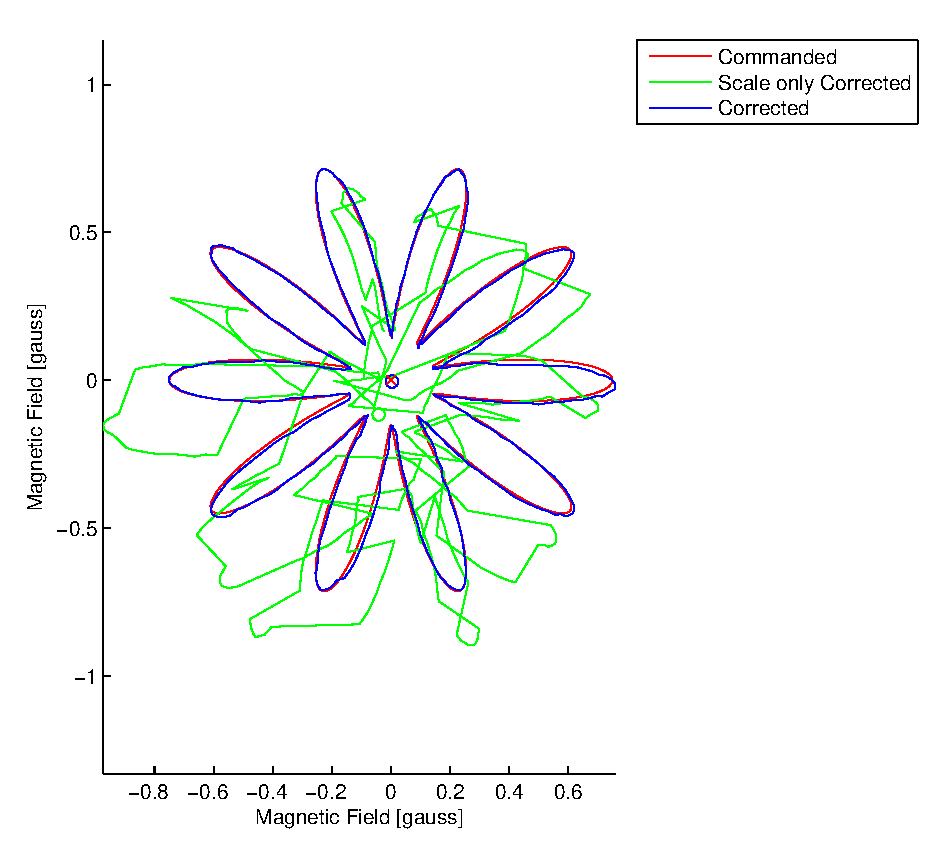
\includegraphics[width=\textwidth]{Figures/torqueCalTst}
    \caption{Torquer Calibration Test Graph}
    \label{fig:tcalTst}
    \todo[inline]{Repeat with fully integrated satellite as it says in the text.}
\end{figure}

\section{Attitude Determination}

The original design did not use attitude determination to get the satellite into the proper orientation. Instead the rotation rates are used along with the bias windows to get the satellite into the right alignment. The problem is that computing the rotation to the needed accuracy is not a simple process. The original idea was that the rotation rates could be computed directly from magnetic field measurements. A set of magnetometer measurements would be taken each time step to compute the rotation rates. The problem is that to do the rotation rate calculation a derivative is needed. Numerical differentiation is possible but it tends to increase noise by acting as a high pass filter.

The proposed rate determination algorithm also falls short because it does not estimate the full rotation rates. Because the magnetic field is used to determine rotation rates rotations around the magnetic field can not be resolved. This was thought not to be an issue because these rotations are also the kind that can not be corrected for by the torquers but it was shown,in simulation, that removing the component of the rotation rates parallel to the magnetic field caused the CubeSat not to stabilize into the proper alignment. 

To solve both of these problems a Kalman filter is used to estimate both the attitude and the rotation rates using the magnetic field data. The Kalman filter estimates the rates by using the assumed satellite dynamics along with a magnetic field model. The Kalman filter uses the knowledge of the system dynamics to smooth the rate estimates and reduce noise. 



\begin{comment}

\begin{equation}
    F_k = 
        \begin{bmatrix}
              0                &   \hat {\omega} _3 & - \hat {\omega} _2  & \frac{1}{2} & 0           & 0           \\
            - \hat {\omega} _3 &   0                &   \hat {\omega} _1  & 0           & \frac{1}{2} & 0           \\
              \hat {\omega} _2 & - \hat {\omega} _1 &   0                 & 0           & 0           & \frac{1}{2} \\
            0 & 0 & 0 & 0                  & K_1 \hat{\omega}_3 & K_1 \hat{\omega}_2 \\
            0 & 0 & 0 & K_2 \hat{\omega}_3 & 0                  & K_2 \hat{\omega}_1 \\
            0 & 0 & 0 & K_3 \hat{\omega}_2 & K_3 \hat{\omega}_1 & 0                  \\
        \end{bmatrix}
\end{equation}

\begin{equation}
    \Phi \left( t \right) = \matt{I} + \matt{F} t = 
        \begin{bmatrix}
              1                  &   \hat {\omega} _3 t & - \hat {\omega} _2 t  & \frac{1}{2} t & 0             & 0             \\
            - \hat {\omega} _3 t &   1                  &   \hat {\omega} _1 t  & 0             & \frac{1}{2} t & 0             \\
              \hat {\omega} _2 t & - \hat {\omega} _1 t &   1                   & 0             & 0             & \frac{1}{2} t \\
            0 & 0 & 0 & 1                    & K_1 \hat{\omega}_3 t & K_1 \hat{\omega}_2 t \\
            0 & 0 & 0 & K_2 \hat{\omega}_3 t & 1                    & K_2 \hat{\omega}_1 t \\
            0 & 0 & 0 & K_3 \hat{\omega}_2 t & K_3 \hat{\omega}_1 t & 1                    \\
        \end{bmatrix}
\end{equation}

\begin{equation}
    \matt{Q} = Q \matt{I}
\end{equation}

\begin{equation}
    \matt{Q}_k = \int _0 ^ {T_s} \matt{\Phi} \left( \tau \right) \matt{Q} \matt{\Phi} \transpose \left( \tau \right) d\tau = Q \int _0 ^ {T_s} \matt{\Phi} \left( \tau \right) \matt{\Phi} \transpose \left( \tau \right) d\tau
\end{equation}


\begin{equation}
    \matt{Q}_k = Q \int _0 ^ {T_s} \matt{\Phi} \left( \tau \right) \matt{\Phi} \transpose \left( \tau \right) d\tau
\end{equation}

\end{comment}
 
\begin{comment}
\begin{figure}[H]
    \centering
    \includegraphics[width=\textwidth]{Figures/test}
    \todo[inline]{Testing Figure}
    \caption{Test Matlab Figure}
\end{figure}

\end{comment}

% vim: filetype=tex spell 

%CubeSat Chapter 
\chapter{Hardware Implementation of the \acf*{ACDS}}\label{ch:CubeSatHardware}

As stated in \cref{ch:BG} the system design from \cite{Mentch11} has been modified for the implementation in this thesis. The only hardware change from \cite{Mentch11} is to use four Alnico1 torquers in each axis instead of two Alnico1 and two vernier torquers as proposed. This does not effect the electrical hardware as both torquer types are the same size and are flipped by the same circuit.

The \ac{ACDS} board for the \ac{ARC} only contains the processor, torquers and drivers. The sensors are located off board and managed by the \ac{LEDL}. The sensor data is sent over the bus to the \ac{ACDS} processor. 

%Both the  \ac{LPMT} and the biasing algorithm have never been flight tested. To test the \ac{LPMT} and bias algorithm the \ac{ARC} will fly an \ac{ACDS} that uses \acp{LPMT}. The central \ac{ACDS} processor and the hardware required to flip the torquers are located on the \ac{ACDS} board while the sensors are located on the \acp{SPB}.

\section{Mechanical Configuration of the \acf*{ARC}}

\Cref{fig:arcMech} shows the mechanical design of the \ac{ARC}. The design has a central board stack with solar panels and rails attached to rings that are on the top and bottom of the board stack. The boards in the stack are connected by a 104-pin \enquote{stack through} header that is located on the -Y edge of each board. The header distributes power and allows for communication between boards. 

\begin{figure}[!ht]
    \centering
    \begin{minipage}{0.33\linewidth}
        \begin{tikzpicture}[remember picture,node distance=0]
            \def\sysx{0.8}
            \node[anchor=south west,inner sep=0] (image) at (0,0) {\includegraphics[width=0.9\linewidth]{cubesat-core}};
            \begin{scope}[x={(image.south east)},y={(image.north west)}]
                % define destination coordinates
                \path (\sysx,0.751) coordinate (LEDL)
                      (\sysx,0.633) coordinate (EPS)
                      (0.86,0.55) coordinate (Z1tq)
                      (0.12,0.55) coordinate (Z2tq)
                      (0.3,0.52) coordinate (Xtq)
                      (\sysx,0.465)  coordinate (ACDS)
                      (0.9,0.4)  coordinate (sep)
                      (\sysx,0.366)  coordinate (COMM)
                      (\sysx,0.281)  coordinate (IMG);
              %draw axis
                \path (0.1,0.12) coordinate (axOrig);
                \draw[->,blue,very thick] (axOrig) to +(-21:0.1) coordinate (X);
                \node[blue,right=of X] (Xl) {X};
                \draw[->,magenta,very thick] (axOrig) to +(196:0.1) coordinate (Y);
                \node[magenta,left=of Y] (Yl) {Y};
                \draw[->,red,very thick] (axOrig) to +(-90:0.1) coordinate (Z);
                \node[red,below=of Z] (Zl) {Z};
              \end{scope}
        \end{tikzpicture}
    \end{minipage}\begin{minipage}{0.65\linewidth}
        \begin{itemize}\setlength{\parskip}{0pt}
            \item[\kern-2em] \tikz[na] \coordinate (LEDLi); \acf{LEDL}
            \item[\kern-2em] \tikz[na] \coordinate (EPSi); \acf{EPS}
            \item[\kern-2em] \tikz[na] \coordinate (ACDSi); \acf{ACDS}
            \item[\kern-2em] \tikz[na] \coordinate (sepi); Separation switch
            %\item[\kern-2em] \tikz[na] \coordinate (ppi); Pull Pin
            \item[\kern-2em] \tikz[na] \coordinate (COMMi); \acf{COMM}
            \item[\kern-2em] \tikz[na] \coordinate (IMGi); \acf{IMG}
        \end{itemize}
    \end{minipage}

    \begin{tikzpicture}[overlay,remember picture]
            \path[->,red,very thick] (LEDLi) edge (LEDL);
            \path[->,red,very thick] (EPSi) edge (EPS);
            \path[->,red,very thick] (ACDSi) edge (ACDS);
            \path[->,red,very thick] (sepi) edge (sep);
            \path[->,red,very thick] (COMMi) edge (COMM);
            \path[->,red,very thick] (IMGi) edge (IMG);
            %draw axis
    \end{tikzpicture}
    \caption{The \acs*{ARC} mechanical setup}
    \label{fig:arcMech}
\end{figure}

The \ac{ACDS} board is located 3rd from the bottom of the stack. This puts it in the center of the board stack. Because the solar cells cover all of the side faces except a small strip in the center this makes the \ac{ACDS} board the only place to put the pull pin and \ac{USB} connector, that need to be accessed while \ac{ARC} is in the \ac{PPOD}. The separation switch connections are also located on the \ac{ACDS} board, as the separation switch is attached to one of the torquer standoffs.

\begin{figure}[!ht]
    \centering
    \begin{minipage}{0.30\linewidth}
        \centering\large{Back}
        \begin{tikzpicture}[remember picture] 
            \node[anchor=south west,inner sep=0] (image) at (0,0) {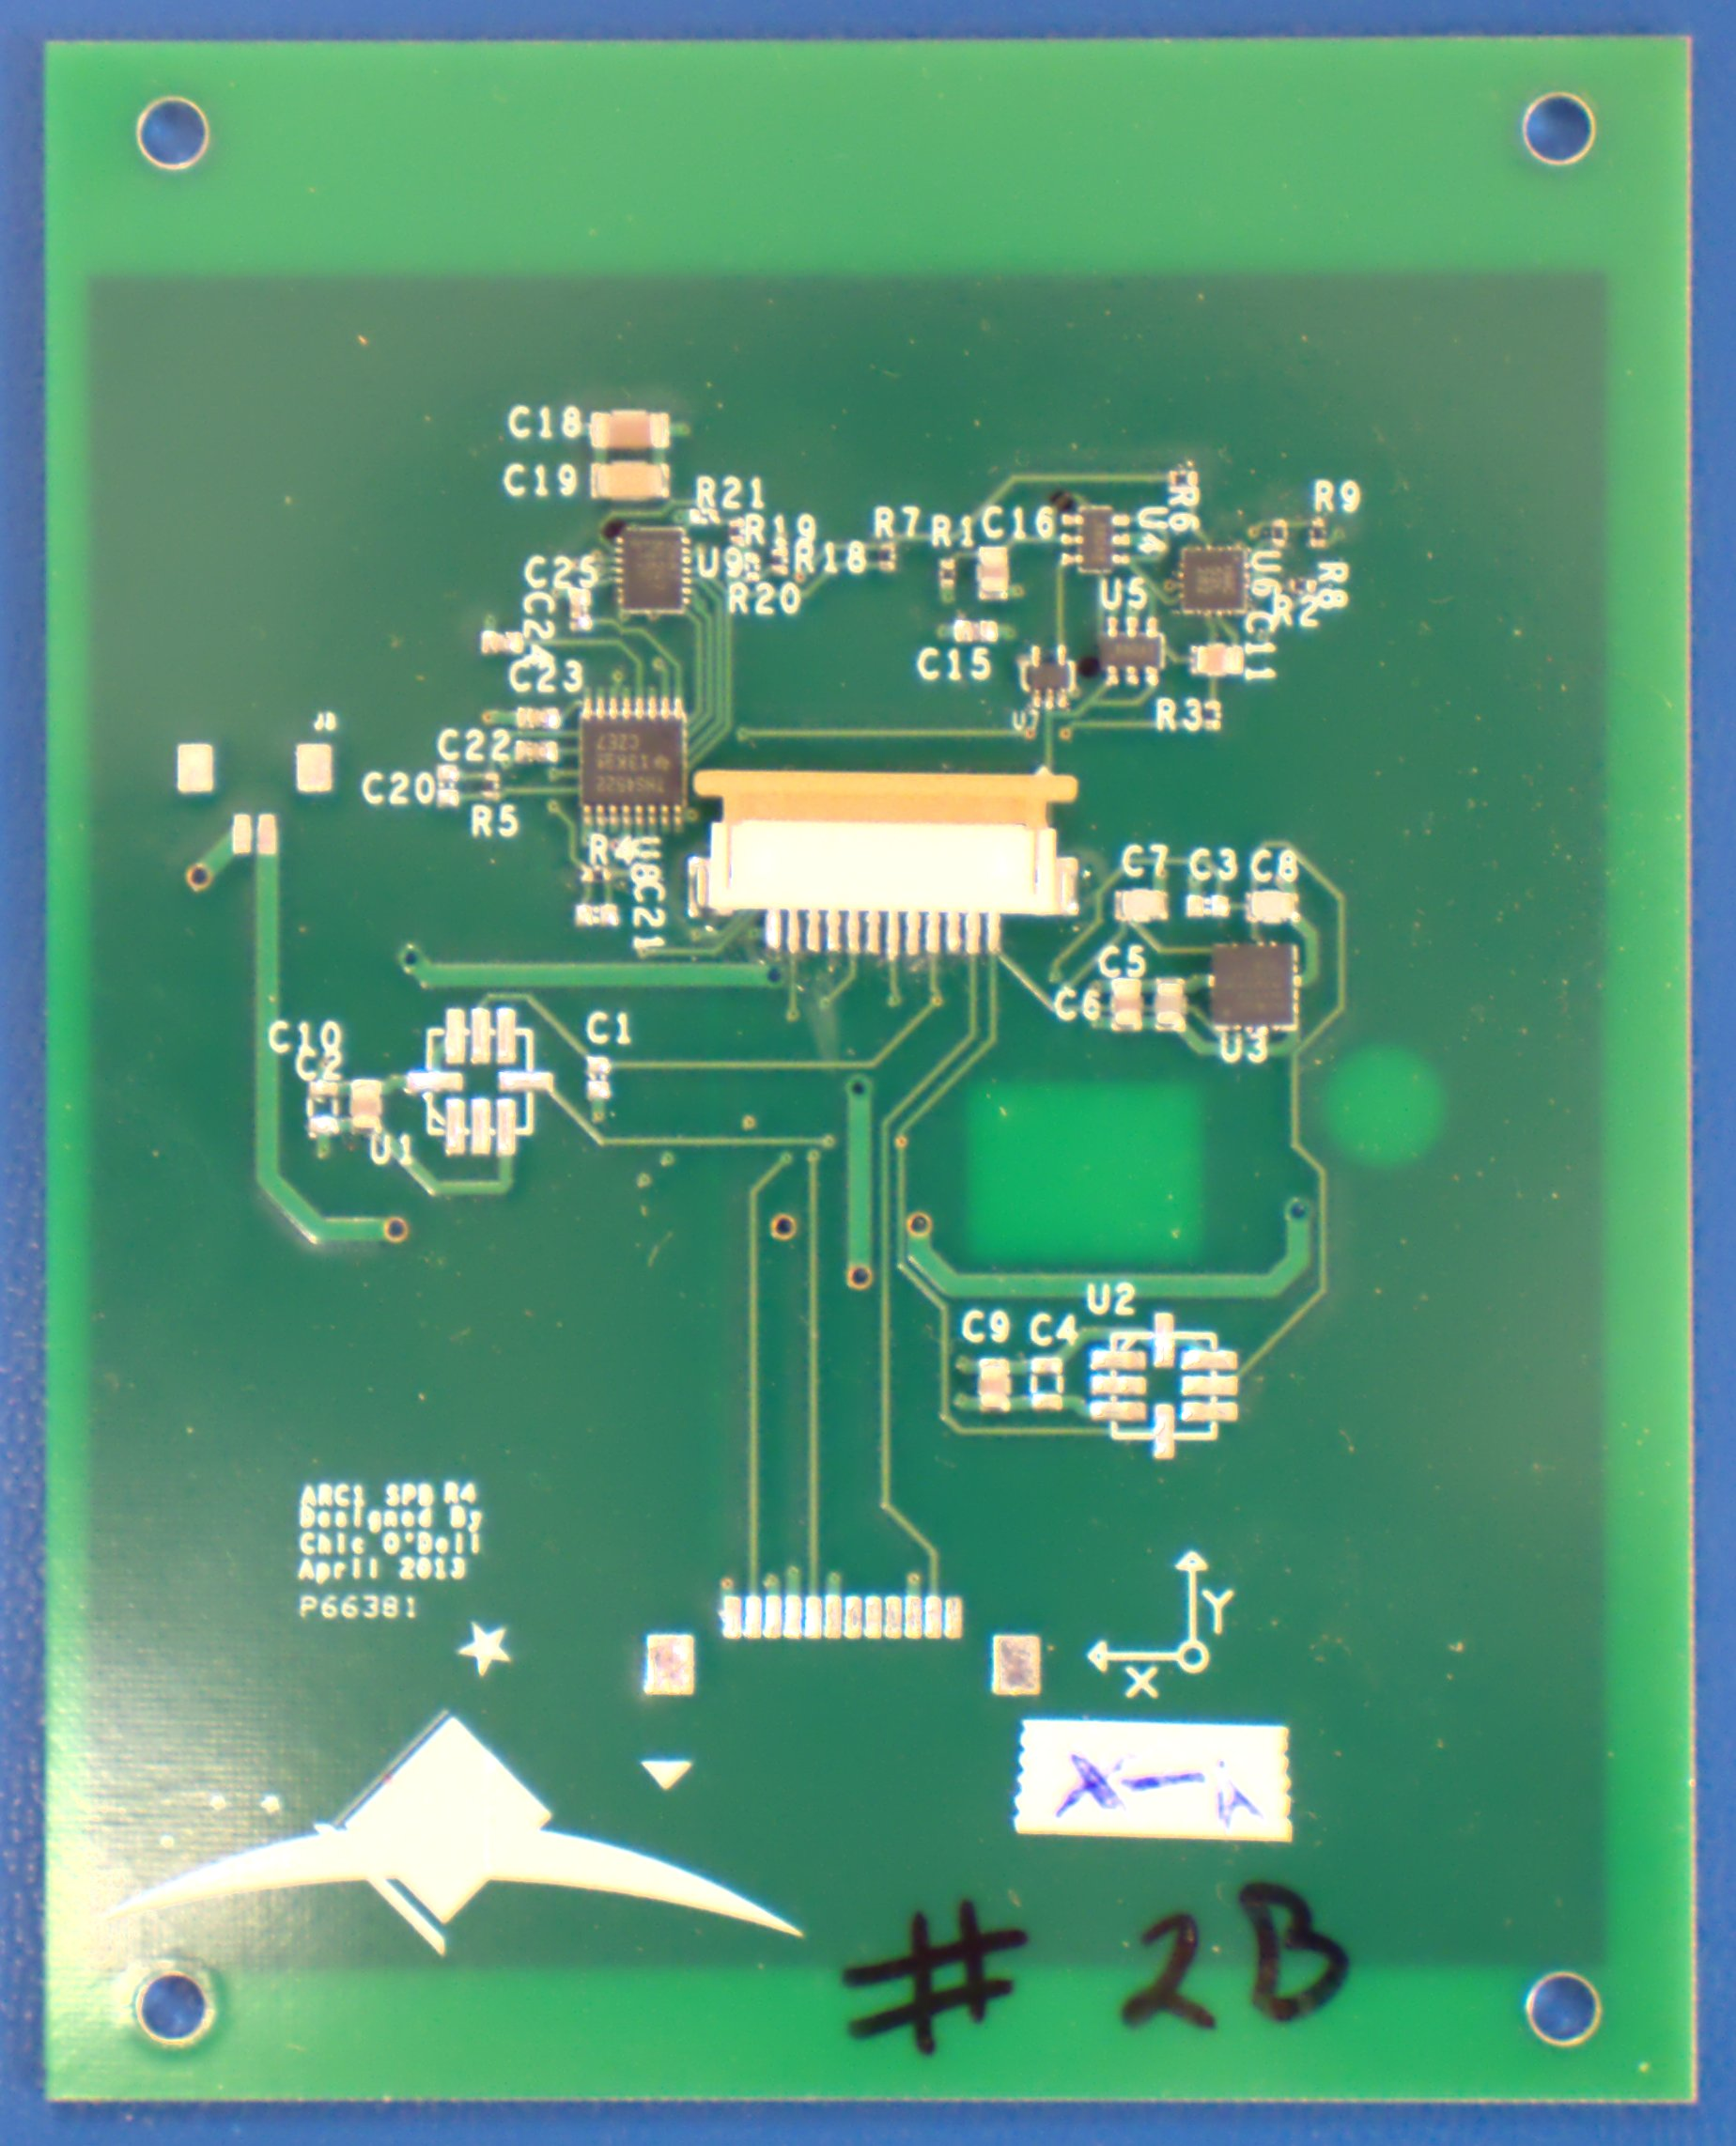
\includegraphics[width=\linewidth]{SPB-back}};
            \begin{scope}[x={(image.south east)},y={(image.north west)}]
                \path (0.715,0.74) coordinate (MAG)
                      (0.395,0.72) coordinate (ADC)
                      (0.395,0.65) coordinate (AMP)
                      (0.745,0.525) coordinate (ACC)
                      (0.615,0.58) coordinate (DAT);
              \end{scope}
        \end{tikzpicture}
    \end{minipage}\begin{minipage}{0.30\linewidth}
        {\large\vspace{1.5em}}
        \vspace*{\fill}
        \begin{itemize}\setlength{\parskip}{0pt}
            \item[\kern-0.2em] Temperature Sensor \tikz[na] \coordinate (TEMPi);
            \item[\kern-0.2em] \tikz[na] \coordinate (MAGi); Magnetometer
            \item[\kern-0.2em] \tikz[na] \coordinate (ADCi); \acs{ADC}
            \item[\kern-0.2em] \tikz[na] \coordinate (AMPi); Amplifier
            \item[\kern-0.2em] Solar Cells \tikz[na] \coordinate (SCi);
            \item[\kern-0.2em] \tikz[na] \coordinate (ACCi); Accelerometer
            \item[\kern-0.2em] \tikz[na] \coordinate (DATi); Data Connector
        \end{itemize}
        \vspace*{\fill}
    \end{minipage} \begin{minipage}{0.30\linewidth}
        \centering\large{Front}
        \begin{tikzpicture}[remember picture] 
            \node[anchor=south west,inner sep=0] (image) at (0,0) {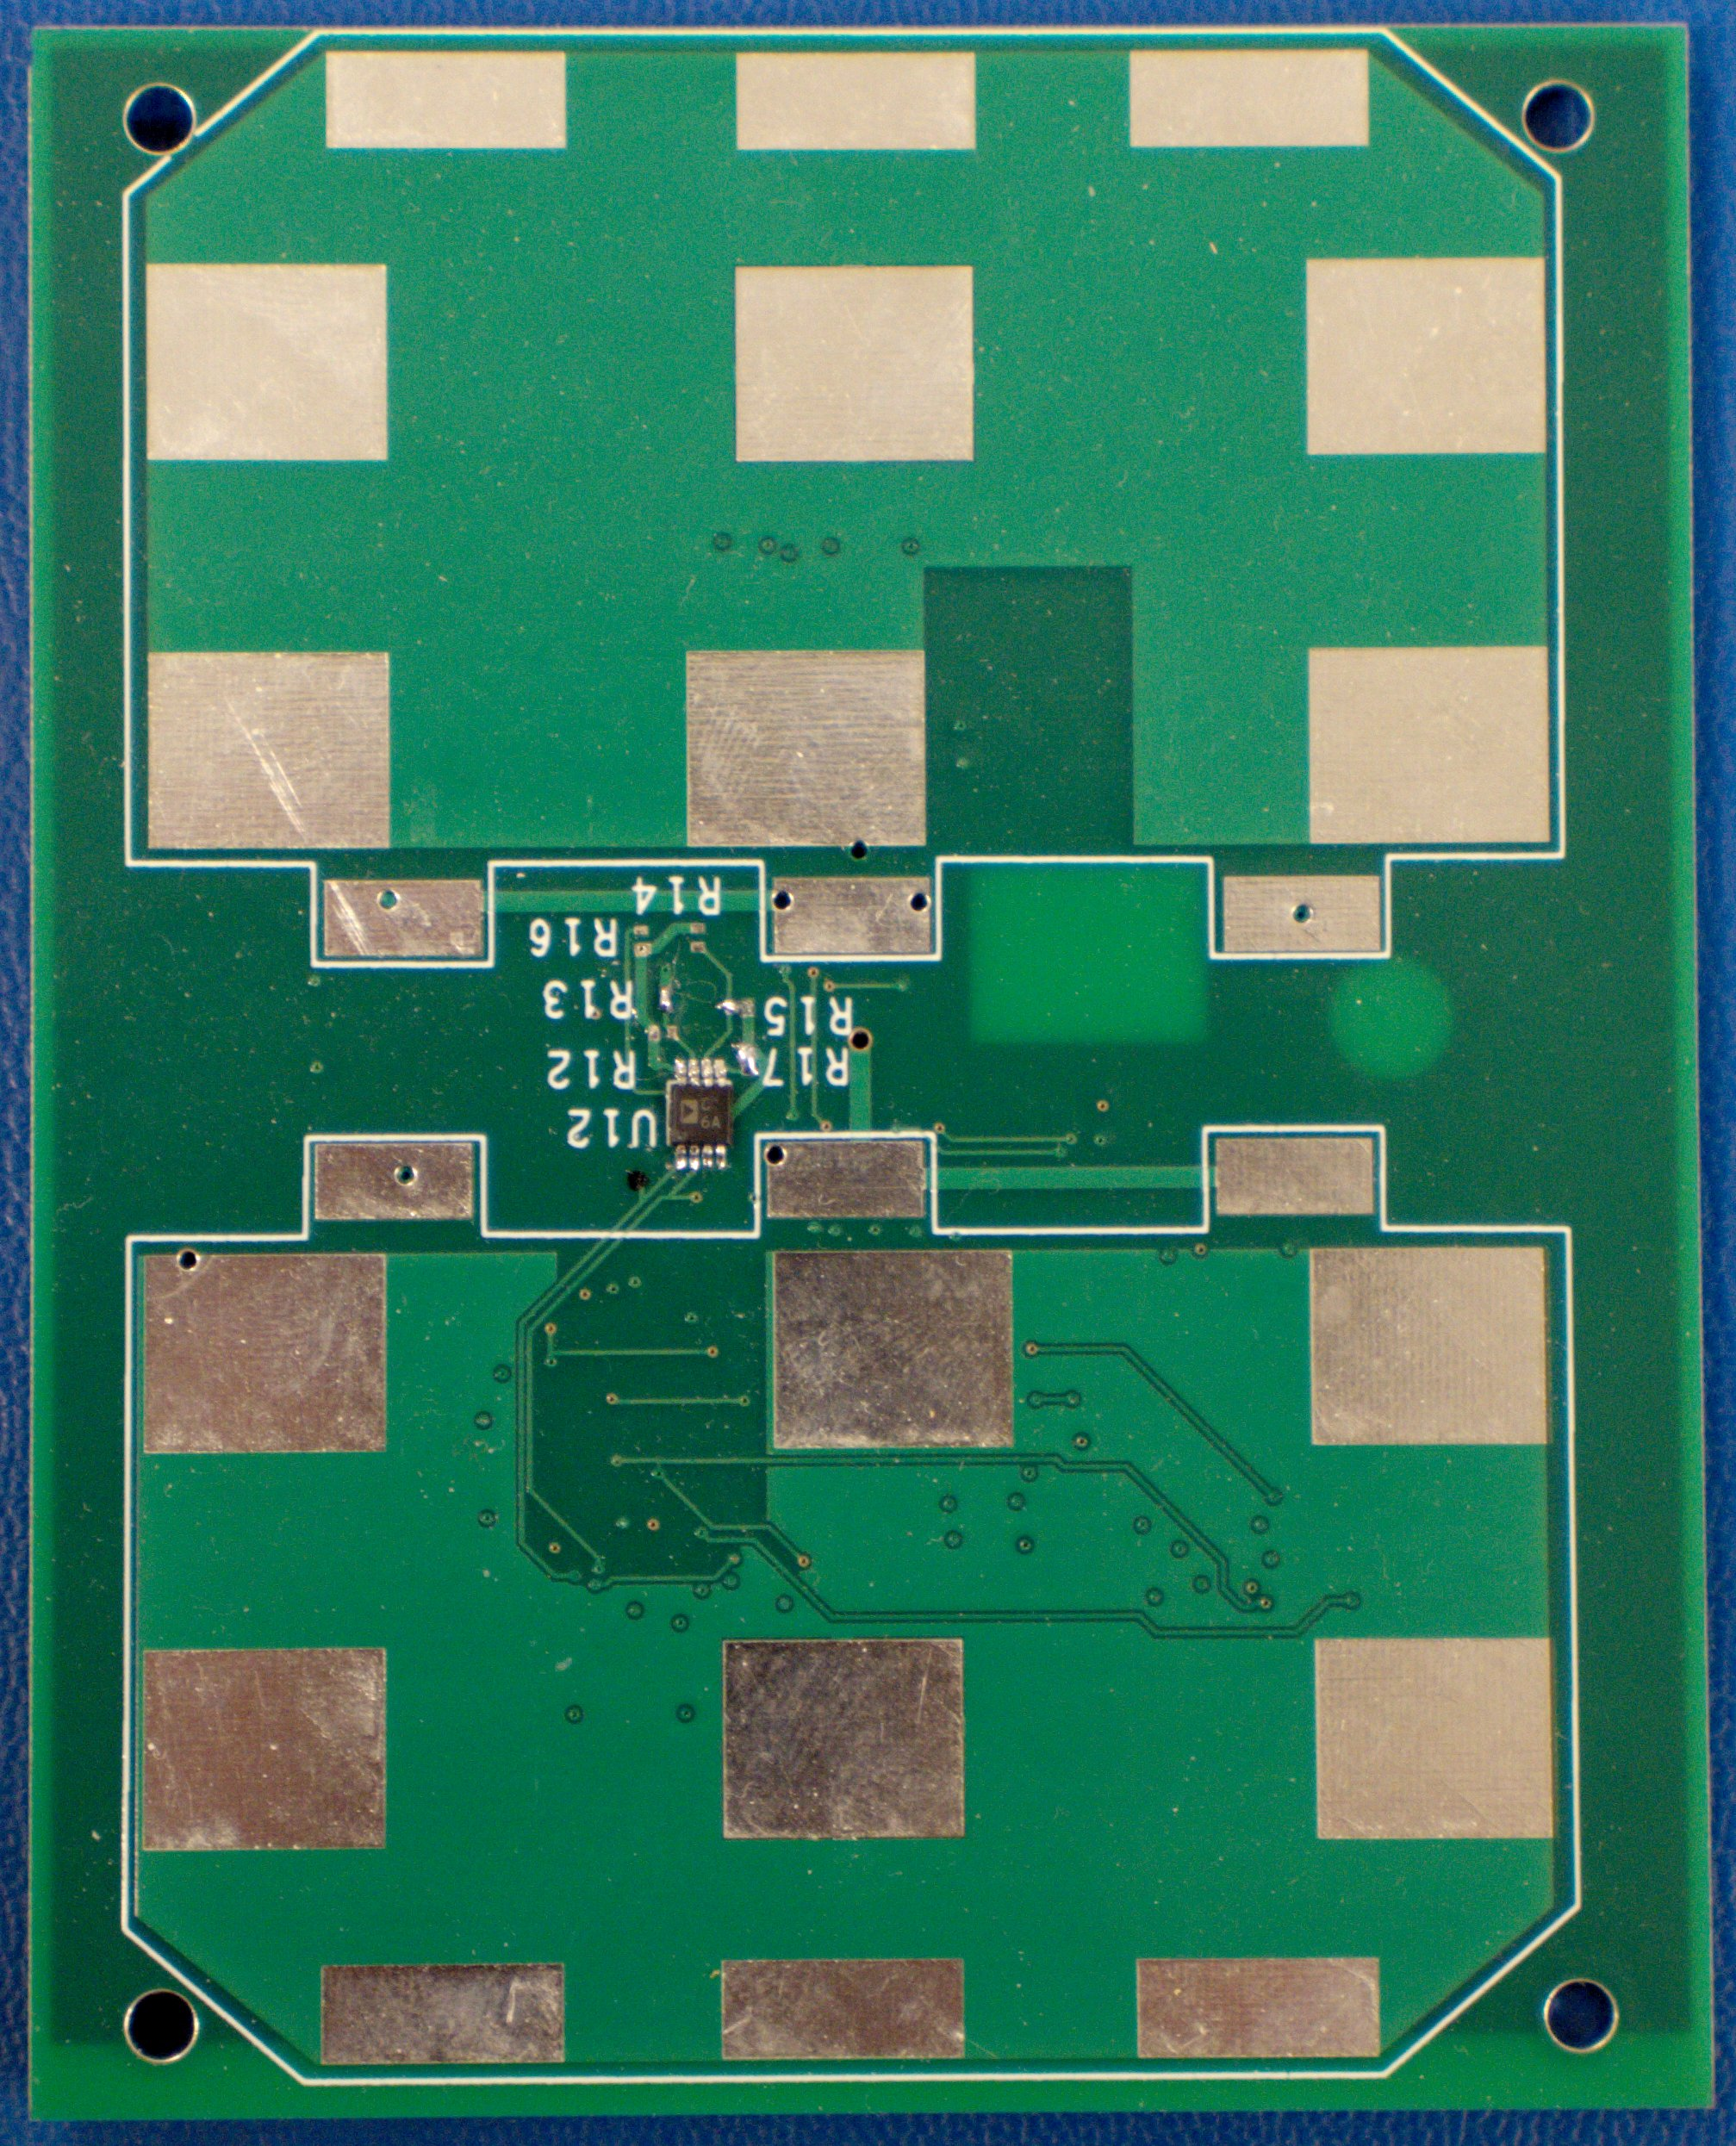
\includegraphics[width=\linewidth]{SPB-front}};
            \begin{scope}[x={(image.south east)},y={(image.north west)}]
                \path (0.39,0.49) coordinate (TEMP)
                      (0.094,0.60) coordinate (SC1)
                      (0.082,0.35) coordinate (SC2);
              \end{scope}
        \end{tikzpicture}
    \end{minipage}

    \begin{tikzpicture}[overlay,remember picture]
            \path[->,red,very thick] (MAGi) edge (MAG);
            \path[->,red,very thick] (ADCi) edge (ADC);
            \path[->,red,very thick] (AMPi) edge (AMP);
            \path[->,red,very thick] (ACCi) edge (ACC);
            \path[->,red,very thick] (DATi) edge (DAT);
            \path[->,red,very thick] (TEMPi) edge (TEMP);
            \path[->,red,very thick] (SCi) edge (SC1);
            \path[->,red,very thick] (SCi) edge (SC2);
    \end{tikzpicture}
    
    \caption{Back and front sides of the Solar Panel Board showing the magnetometer location.}
    \label{fig:SPB}
\end{figure}

For clarity the \acp{SPB} are not shown in \cref{fig:arcMech}. The \acp{SPB} are attached to mounting holes in the rails and are the outer faces of the \ac{ARC}. In addition to the solar cells the \acp{SPB} also contain sensors that are used by the \ac{LEDL} and \ac{ACDS}. \Cref{fig:SPB} shows the back side of a side \ac{SPB} with the sensors labeled, and the front side showing the temperature sensor and the pads where the solar cells will mount. The top and bottom \acp{SPB} are similar to the side \acp{SPB} except they lack accelerometers and include parts for the antennas and antenna deployment.

The core board stack contains the major subsystems for the \ac{ARC}. Some of these subsystems are designed to carry out a specific \ac{SMO} while others provide a general support role. The subsystems are as follows:

\begin{description}
    \item[\acs{LEDL} :] One of the \acp{SMO} on \ac{ARC} is to \enquote{Characterize the thermal and vibration environment inside the launch vehicle from ignition to orbit insertion.}\cite{ARCweb} The \ac{LEDL} does this by using a separate battery to operate during the launch phase and log data from accelerometers and temperature sensors.
    \item[\acs{EPS} :] The \ac{EPS} manages the electrical power on \ac{ARC}. The solar cells connect to \acp{BCR} which have peak power point tracking and output the proper voltage to charge the batteries. The voltage from the batteries is regulated down to 5~V and 3.3~V. The \ac{EPS} supplies the unregulated battery voltage along with the 5~V and 3.3~V rails to the rest of the satellite. The \ac{EPS} is the only system on the \ac{ARC} not built at UAF. The \ac{EPS} is designed and built by Clyde Space. \cite{ClydeEPS}
    \item[\acs{ACDS} :] One of the \acp{SMO} on \ac{ARC} is to \enquote{Validate a novel low power \acf{ACDS}.} \cite{ARCweb} This is the system discussed in this thesis.
    \item[Separation Switch :] This switch is screwed into one of the torquer standoffs and cuts off power to the CubeSat when it is in the \ac{PPOD}.
    \item[\acs{COMM} :] The \ac{COMM} allows for two-way communication with the ground. A 9600~bps command/beacon up/down link and a 38400~bps data down link are used. The 9600~bps link operates on the 436~MHz band and uses a tape measure monopole. The 38400~bps link operates on the 2.4~GHz and uses a ceramic patch antenna mounted on the bottom of the \ac{ARC}.
    \item[\acs{IMG} :] One of the \acp{SMO} on the \ac{ARC} is to \enquote{Validate a high bandwidth communication system by obtaining images of changing snow/ice coverage in arctic regions.}\cite{ARCweb} The imager has a camera and an \ac{SD}. The camera is used to take pictures and store them on the \ac{SD}.
\end{description}

The \ac{EPS} is designed and manufactured by Clyde Space as a generic CubeSat \ac{EPS}. The \ac{EPS} is compatible with CubeSat Kit\cite{CSK} hardware which is one of the main standards for off-the-shelf CubeSat hardware. Because of this the rest of the \ac{ARC} subsystems must be compatible with the CubeSat Kit hardware. All boards have the same header and mounting hole locations and similar outlines so that they all fit together in the CubeSat.

\subsection{\acl*{ARC} \acl*{ACDS} Hardware}

The \ac{ACDS} board has the same overall outline and hole pattern as the rest of the \ac{ARC} subsystems but, it has 4 notches cut out to accommodate the Z-axis torquers and torquer standoffs. Additionally, there is a bump-out for the \ac{USB} connector so that it can be closer to the access port to allow a \ac{USB} cable to be easily plugged in.

\begin{figure}[!ht]
    \centering
    \begin{minipage}{0.38\linewidth}
        \raggedleft
        \vspace{4em}
        \begin{itemize}\setlength{\parskip}{0pt}
            \item[\kern-0.2em] X torquers \tikz[na] \coordinate (TqXi);
            \item[\kern-0.2em] Pull Pin Housing \tikz[na] \coordinate (PPi);
            \item[\kern-0.2em] \acf{USB} connection \tikz[na] \coordinate (USBi);
        \end{itemize}
    \end{minipage}\begin{minipage}{0.32\linewidth}
        \begin{tikzpicture}[remember picture] 
            \node[anchor=south west,inner sep=0] (image) at (0,0) {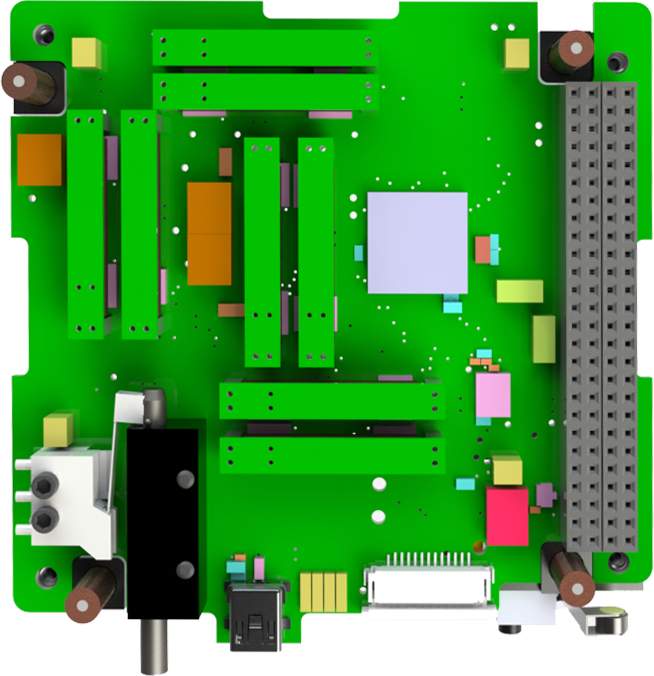
\includegraphics[width=\linewidth]{ACDS-board-render}};
            \begin{scope}[x={(image.south east)},y={(image.north west)}]
                \path (0.19,0.35) coordinate (PP)
                      %(0.30,0.27) coordinate (PP)
                      (0.39,0.09) coordinate (USB)
                      (0.45,0.70) coordinate (TqX1)
                      (0.36,0.70) coordinate (TqX2)
                      (0.18,0.70) coordinate (TqX3)
                      (0.25,0.70) coordinate (TqX4)
                      (0.45,0.895) coordinate (TqY1)
                      %(0.45,0.89) coordinate (TqY1)
                      (0.45,0.93) coordinate (TqY2)
                      (0.50,0.37) coordinate (TqY3)
                      (0.50,0.49) coordinate (TqY4)
                      (0.14,0.13) coordinate (TqZ1)
                      (0.05,0.87) coordinate (TqZ2)
                      (0.88,0.90) coordinate (TqZ3)
                      (0.89,0.15) coordinate (TqZ4)
                      (0.96,0.095) coordinate (SS);
              %draw axis
                %\path (0.15,0.72) coordinate (axOrig);
                %\draw[->,red,very thick] (axOrig) to +(-88.3:0.1) coordinate (X);
                %\node[red,below=of X] (Xl) {X};
                %\draw[->,magenta,very thick] (axOrig) to +(180.5:0.1) coordinate (Y);
                %\node[magenta,left=of Y] (Yl) {Y};
                %\draw[->,red,very thick] (axOrig) to +(-90:0.1) coordinate (Z);
                %\node[red,below=of Z] (Zl) {Z};
              \end{scope}
        \end{tikzpicture}
    \end{minipage}\begin{minipage}{0.30\linewidth}
        \begin{itemize}\setlength{\parskip}{0pt}
            %\item[\kern-0.2em] \tikz[na] \coordinate (TqXi); X torquers
            \item[\kern-0.2em] \tikz[na] \coordinate (TqYi); Y torquers
            \item[\kern-0.2em] \tikz[na] \coordinate (TqZi); Z torquers
            \item[\kern-0.2em] \tikz[na] \coordinate (SSi); Separation switch
            %\item[\kern-0.2em] \tikz[na] \coordinate (PPi); Pull Pin
            %\item[\kern-0.2em] \tikz[na] \coordinate (USBi); \acf{USB} connection
        \end{itemize}
    \end{minipage}

    \begin{tikzpicture}[overlay,remember picture]
            \path[->,blue,very thick] (PPi) edge (PP);
            \path[->,blue,very thick] (USBi) edge (USB);
            \path[->,red,very thick] (TqXi) edge (TqX1);
            %\path[->,red,very thick] (TqXi) edge (TqX2);
            \path[->,red,very thick] (TqXi) edge (TqX3);
            %\path[->,red,very thick] (TqXi) edge (TqX4);
            \path[->,black,very thick] (TqYi) edge (TqY1);
            %\path[->,black,very thick] (TqYi) edge (TqY2);
            \path[->,black,very thick] (TqYi) edge (TqY3);
            %\path[->,black,very thick] (TqYi) edge (TqY4);
            \path[->,magenta,very thick] (TqZi) edge (TqZ1);
            \path[->,magenta,very thick] (TqZi) edge (TqZ2);
            \path[->,magenta,very thick] (TqZi) edge (TqZ3);
            \path[->,magenta,very thick] (TqZi) edge (TqZ4);
            \path[->,blue,very thick] (SSi) edge (SS);
    \end{tikzpicture}
    \caption{The \ac{ARC} \ac{ACDS} board.}
    \label{fig:boardRender}
\end{figure}

In addition to the \ac{ACDS} hardware, the \ac{ACDS} board also is the connection point for the pull pin, separation switch, and \ac{USB} connection port. These are located on the \ac{ACDS} board because it is the only board that is accessible through the \ac{SPB}. The pull pin, separation switch, and \ac{USB} connection connect directly to the header and are not connected to the core \ac{ACDS} hardware. The \ac{USB} Port is used for charging and satellite diagnostics during testing and on the ground. The Pull Pin, when inserted, keeps the satellite powered off until it is inserted into the \ac{PPOD} after which the separation switch keeps the satellite powered off until orbital insertion.

The Z-axis torquers are housed inside the standoffs which are located on the four corners of the board. The \ac{ACDS} board shape has been modified from the standard board shape to accommodate the torquers and standoffs. This is visible in \cref{fig:boardRender}. The notches are designed to fit the z-axis torquer standoffs and keep them aligned in the proper orientation. The torquers fit into a hole drilled into the standoffs and are held in place with epoxy. 

\subsection{Bus Communication}

The subsystems of the \ac{ARC} will communicate with each other using the ARCBus. The ARCBus consists of shared connections between the subsystems to transmit commands and data. The ARCBus will be primarily used by the \ac{ACDS} to get sensor data from the \ac{LEDL} and send and receive data to the ground station through the COMM system. Commands are transmited using an \ac{I2C} bus and large blocks of data are transfered using a \ac{SPI} bus which is negotiated using the \ac{I2C} bus.

\section{Components of the \acl*{ACDS}}

\afterpage{\begin{landscape}
\begin{figure}[p!]
    \centering
    % vim: filetype=tex spell 

% We need layers to draw the block diagram
\pgfdeclarelayer{background}
\pgfdeclarelayer{foreground}
\pgfdeclarelayer{Hardware}
\pgfdeclarelayer{CPU}

\pgfsetlayers{background,Hardware,CPU,main,foreground}

\begin{tikzpicture}
    %first draw ARCbus
    \begin{pgfonlayer}{Hardware}
        \node[draw=black,minimum height=10cm,minimum width=1cm] (arcbus) at (0,0) {\rotatebox{90}{\acs{ARC} Bus}};
    \end{pgfonlayer}

    \begin{scope}[start chain]
        \node[perif,node distance=1.5cm,right=of arcbus]    (SPI_IIC)  {\rotatebox{90}{\acs{SPI} + \acs{I2C}}};
        \node[prog]    (command) at ([yshift=15mm,xshift=3mm]SPI_IIC) {command and control};

        \begin{scope}[start branch=storage going below]
            \node[point,node distance=15mm,on chain] (nexus) {};
            \node[prog,text width=7em,node distance=5mm,on chain=going right]       (housek)   {Housekeeping};
            \node[perif,node distance=2mm]    (SPI)      {\acs{SPI}};
            \node[hardware]    (SD)       {\acs{SD}};
        \end{scope}

        \node[prog]    (lpmt)     {\acs{LPMT} algorithm};
        \node[perif,join=by dataL]       (tqio)    {\rotatebox{90}{\acs{GPIO}}};
        \node[hardware,join=by dataL]    (hbridge)    {H-Bridges};

        \begin{scope}[start branch=power going left]
            \node [power,on chain=going above]   (cap) {Capacitors (one per axis)};
            \node [power]      (capchg) {Capacitor charging circuit};
        \end{scope}

        \node[hardware,on chain=going below]    (torquers)    {Torquers};

    \end{scope}

    \begin{scope}[start chain=LEDL going below]
        \node[hardware,node distance =2cm,left=of arcbus]  (LEDL)  {\acs{LEDL} \textmu{}C};
        \begin{scope}[start branch=gyro going above]
            \node[hardware,node distance=5mm]   (gyro) {Gyros};
        \end{scope}
        \node[hardware,text width=8em]   (mag) at ([yshift=-1.5cm]LEDL)     {Magnetometer};
    \end{scope}

    %draw CPU box
    \begin{pgfonlayer}{CPU}
        \node (push) at ([yshift=1.3cm]command) {};
        \node[CPU,fit=(SPI_IIC) (command) (lpmt) (housek) (SPI) (tqio) (push)] (cpu) {};
        \node[above,anchor=south west] at (cpu.north west) {\acs{ACDS} \textmu{}C};
    \end{pgfonlayer}

    %draw board boxes
    \begin{pgfonlayer}{Hardware}
        %draw LEDL board
        \node[PCB,fit=(LEDL) (gyro)] (LEDLpcb) {};
        \node[above,anchor=south west] at (LEDLpcb.north west) {\acs{LEDL}};
        %draw SPB
        \node[PCB,fit=(mag)] (spb) {};
        \node[above,anchor=south west] at (spb.north west) {\acs{SPB}};
        %draw ACDS
        \node[PCB,fit=(cpu) (SD) (hbridge) (cap) (capchg) (torquers)] (ACDSpcb) {};
        \node[above,anchor=south west] at (ACDSpcb.north west) {\acs{ACDS}};
    \end{pgfonlayer}

    \begin{pgfonlayer}{foreground}
        \node[draw=black,fill=white] (legend) at ([xshift=-2cm]ACDSpcb.south east) {\begin{tikzpicture}
            \begin{scope}[start chain=going below,node distance=1mm]
                \node[power,text width=6em] (cleg) {Power Component};
                \node[prog,text width=6em] {Program Component};
                \node[perif,text width=6em] {Peripheral};
                \node[hardware,text width=6em,minimum height=1em] {Hardware};
            \end{scope}
            \begin{scope}[start chain=going below,node distance=0cm,text width=6em]
                \node[on chain,left=of cleg] {};

                \node[on chain,rectangle] (pl) {Power Line};
                \path[powerL] (pl.west) ++(-5mm,0) -- ++(-1cm,0);

                \node[on chain,rectangle] (dl) {Data Line};
                \path[dataL] (dl.west) ++(-5mm,0) -- ++(-1cm,0);

                \node[on chain,rectangle] (bl) {Bus Line};
                \path[Bus] (bl.west) ++(-5mm,0) -- ++(-1cm,0);
            \end{scope}
            
        \end{tikzpicture}};
        \node[anchor=north west] at (legend.north west) {\large \bf Legend};
    \end{pgfonlayer}

    \path[Bus] (LEDL) -- (arcbus);
    \path[Bus] (SPI_IIC) -- (arcbus);
    \path[Bus] (LEDL) -- (mag);
    \path[dataL] (LEDL) -- (gyro);

    %dummy nodes for getting good connections
    \node[point] (shift1) at ([yshift=8mm]housek) {};
    \node[point] (shift2) at ([xshift=-8mm]nexus) {};

    \path[dataL] (SPI_IIC.north) |- (command.west);
    \path[dataL] (SPI_IIC) -| (shift2);
    \path[dataL] (nexus) -- (housek);
    \path[dataL] (lpmt.south) |- (shift1);
    \path[dataL] (command.south) |- (shift1);
    \path[dataL] (shift1) -- (housek);
    \path[dataL] (shift2) -- (housek);
    \path[dataL] (command) -- (lpmt);
    \path[dataL] (housek) -- (SPI);
    \path[dataL] (SPI) -- (SD);

    \path[powerL] (capchg) -- (cap);
    \path[powerL] (cap) -- (hbridge);
    \path[powerL] (hbridge) -- (torquers);

\end{tikzpicture}



    \caption{Block Diagram of the CubeSat \acs*{ACDS} system}
    \label{fig:ACDS-block}
\end{figure}
\end{landscape}}

The block diagram for the CubeSat hardware used to implement the \ac{ACDS} is shown in \cref{fig:ACDS-block}. The hardware necessary for the \ac{ACDS} is spread over multiple subsystems of the \ac{ARC}. The \ac{ACDS} board contains the torquers and, driving hardware along with the microcontroller which will run the attitude control algorithm. There is one two-axis magnetometer located on each of the six \acp{SPB}. These are used by the \ac{ACDS} to calculate rotation rates and calculate the magnetic dipole moment required to generate the necessary torque. Spreading the magnetometers across all six faces should give some degree of noise immunity and redundancy. The \ac{LEDL} board also contains \ac{MEMS} angular rate sensors as a redundant measurement of the rotation rate of the \ac{ARC}. The sensors on the \acp{SPB} are read by the \ac{LEDL}, which then forwards the magnetometer and angular rate measurements to the \ac{ACDS}.

\section{Torquers}

\Cref{fig:torquers} illustrates the torquer locations within the \ac{ARC}. The torquers consist of a hard magnetic core surrounded with a coil of wire. There are a total of twelve torquers on the \ac{ARC}, with four in each axis. The torquers are flipped using a driving circuit that causes a current pulse to flow through the coil. The driving hardware for the torquers is designed to flip one torquer in each axis every second.

\begin{figure}[!htbp]
    \centering
    \begin{minipage}{0.27\linewidth}
        \begin{itemize}\setlength{\parskip}{3pt}
            \item[\kern-0.2em] Magnetometers \tikz[na] \coordinate (MAGi);
            \item[\kern-0.2em] X torquers \tikz[na] \coordinate (XTi);
            \item[\kern-0.2em] Y torquers \tikz[na] \coordinate (YTi);
            \item[\kern-0.2em] Z torquers\tikz[na] \coordinate (ZTi);
        \end{itemize}
        \vspace{1em}
    \end{minipage}\begin{minipage}{0.68\linewidth}
        \begin{tikzpicture}[remember picture] 
            \node[anchor=south west,inner sep=0] (image) at (0,0) {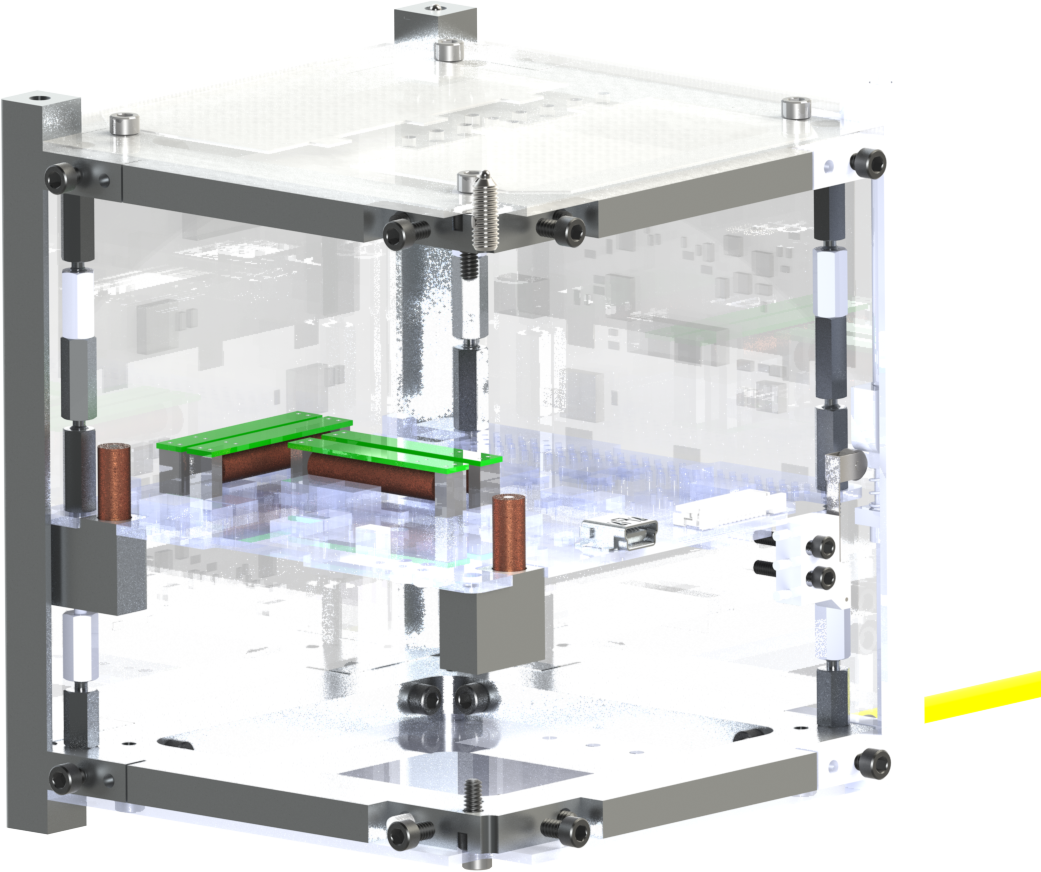
\includegraphics[width=\linewidth]{torquers}};
            \begin{scope}[x={(image.south east)},y={(image.north west)}]
                \fill[blue,fill opacity=0.3] (0.725,0.758) -- (0.744,0.757) -- (0.743,0.731) -- (0.725,0.732) -- cycle;
                \fill[blue,fill opacity=0.3] (0.183,0.763) -- (0.2015,0.7635) -- (0.202,0.739) -- (0.184,0.738) -- cycle;
                \path (0.725, 0.742) coordinate (MAG1)
                      (0.183, 0.742) coordinate (MAG2)

                      (0.26,0.55) coordinate (XT1)
                      (0.41,0.57) coordinate (XT2)

                      (0.288,0.59) coordinate (YT1)
                      (0.528,0.54) coordinate (YT2)

                      (0.115,0.51) coordinate (ZT1)
                      (0.48,0.4) coordinate (ZT2)
                      (0.45,0.61) coordinate (ZT3)
                      (0.77,0.54) coordinate (ZT4);
              \end{scope}
        \end{tikzpicture}
    \end{minipage}

    \begin{tikzpicture}[overlay,remember picture]
            \path[->,red,very thick] (MAGi) edge (MAG1);
            \path[->,red,very thick] (MAGi) edge (MAG2);

            \path[->,blue,very thick] (XTi) edge (XT1);
            \path[->,blue,very thick] (XTi) edge (XT2);

            \path[->,black,very thick] (YTi) edge (YT1);
            \path[->,black,very thick] (YTi) edge (YT2);

            \path[->,magenta,very thick] (ZTi) edge (ZT1);
            \path[->,magenta,very thick] (ZTi) edge (ZT2);
            \path[->,magenta,very thick] (ZTi) edge (ZT3);
            \path[->,magenta,very thick] (ZTi) edge (ZT4);
    \end{tikzpicture}
    
    \caption{Torquer locations within the \ac{ARC}}
    \label{fig:torquers}
\end{figure}

\Cref{fig:TQloc} shows the location and identification designator of each torquer on the \ac{ACDS} board. This is how the torquers are referred to in software.

\begin{figure}[!htbp]
    \centering
    \begin{minipage}{1.7em}
        \setlength{\parskip}{2mm}
        Z1 \tikz[na] \coordinate (Z1i);

        X2 \tikz[na] \coordinate (X2i);

        X1 \tikz[na] \coordinate (X1i);

        X3 \tikz[na] \coordinate (X3i);

        X4 \tikz[na] \coordinate (X4i);

        Z2 \tikz[na] \coordinate (Z2i);
    \end{minipage}\hspace{2em}\begin{minipage}{0.35\linewidth}
        \centering
        \begin{tikzpicture}[remember picture] 
            \node[anchor=south west,inner sep=0] (image) at (0,0) {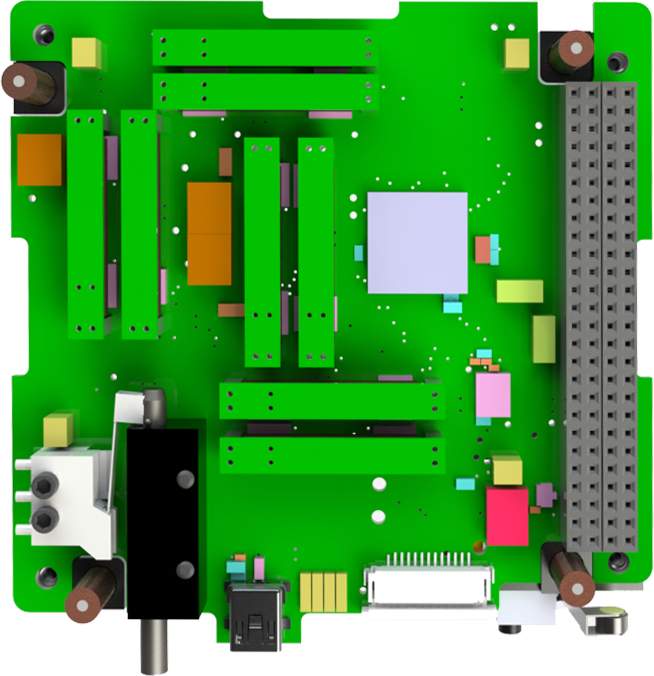
\includegraphics[width=\linewidth]{ACDS-board-render}};
            \begin{scope}[x={(image.south east)},y={(image.north west)}]
                \path 
                      (0.40,0.64) coordinate (X1)
                      (0.48,0.71) coordinate (X2)
                      (0.13,0.58) coordinate (X3)
                      (0.21,0.53) coordinate (X4)
                      (0.45,0.87) coordinate (Y1)
                      (0.45,0.93) coordinate (Y2)
                      (0.50,0.33) coordinate (Y3)
                      (0.50,0.40) coordinate (Y4)
                      (0.01,0.88) coordinate (Z1)
                      (0.11,0.10) coordinate (Z2)
                      (0.90,0.92) coordinate (Z3)
                      (0.90,0.12) coordinate (Z4);
              %draw axis
                %\path (0.15,0.72) coordinate (axOrig);
                %\draw[->,red,very thick] (axOrig) to +(-88.3:0.1) coordinate (X);
                %\node[red,below=of X] (Xl) {X};
                %\draw[->,magenta,very thick] (axOrig) to +(180.5:0.1) coordinate (Y);
                %\node[magenta,left=of Y] (Yl) {Y};
                %\draw[->,red,very thick] (axOrig) to +(-90:0.1) coordinate (Z);
                %\node[red,below=of Z] (Zl) {Z};
              \end{scope}
        \end{tikzpicture}
    \end{minipage}\hspace{2em}\begin{minipage}{1.7em}
        \setlength{\parskip}{2mm}
        \tikz[na] \coordinate (Z3i); Z3

        \tikz[na] \coordinate (Y2i); Y2

        \tikz[na] \coordinate (Y1i); Y1

        \tikz[na] \coordinate (Y4i); Y4

        \tikz[na] \coordinate (Y3i); Y3

        \tikz[na] \coordinate (Z4i); Z4
    \end{minipage}

    \begin{tikzpicture}[overlay,remember picture]
            \path[->,blue,very thick] (X1i) edge (X1);
            \path[->,blue,very thick] (X2i) edge (X2);
            \path[->,blue,very thick] (X3i) edge (X3);
            \path[->,blue,very thick] (X4i) edge (X4);

            \path[->,black,very thick] (Y1i) edge (Y1);
            \path[->,black,very thick] (Y2i) edge (Y2);
            \path[->,black,very thick] (Y3i) edge (Y3);
            \path[->,black,very thick] (Y4i) edge (Y4);

            \path[->,magenta,very thick] (Z1i) edge (Z1);
            \path[->,magenta,very thick] (Z2i) edge (Z2);
            \path[->,magenta,very thick] (Z3i) edge (Z3);
            \path[->,magenta,very thick] (Z4i) edge (Z4);
    \end{tikzpicture}
    \caption{The \ac{ARC} \ac{ACDS} torquer locations.}
    \label{fig:TQloc}
\end{figure}

\subsection{Cores}

Most magnetic torquers use either an air core or a soft magnetic core. Ideally both an air or a soft core only produce torque while a current is running through the coil. A soft core will produce more torque for the same geometry and current compared to an air core. However, soft magnetic materials have some hysteresis that will continue to produce undesired torque after current stops flowing. Hard magnetic materials are chosen to have a large amount of hysteresis so that torque is still produced after the current stops flowing in the coil.

The torquer cores for the \ac{ARC} are made of Alnico1, which is a hard magnetic material. Core materials are chosen for their residual induction ($B_r$) and their coercive force ($H_c$). The torque produced for a given torquer geometry is proportional to $B_r$. This means that $B_r$ dictates the range of torques that are feasible. If $B_r$ is too small, then the torquers will have to be too big to fit in the satellite. If $B_r$ is too large, then it may not be possible to manufacture torquers that are small enough to give the desired torque. The current required to flip the torquer for a given coil and core geometry is determined by $H_c$. It is desirable to have a low $H_c$ so less energy is used for each flip. However, if $H_c$ is too low then the torquer can be flipped inadvertently.

\subsubsection{Core Sizing}

The proposed torquer cores consisted of a large and a small pair in each axis. The large pair were to be made of Alnico1 and produce a magnetic dipole moment of $0.022 \unit{A \cdot m^2}$. The small pair was proposed to have an inert core with a thin permalloy coating to give it a dipole moment of $0.00011 \unit{A \cdot m^2}$. All torquer cores were to be the same size, one inch long of $\sfrac{1}{16}$-inch diameter rod.

As discussed in \cite{Mentch11} the large cores were sized by first determining the desired torque for each torquer, and to produce then calculating the necessary dipole moment. Simulation was used to refine the required dipole moment. Alnico5 was the core material that had been used in previous experiments for much larger cores\cite{Mentch11}\todo{Look for other reference?}. The minimum manufactured size of Alnico rods is $\sfrac{1}{16}$-inch. It is desirable to have a length-to-diameter ratio greater than 10, which fixes the minimum torque that can be achieved. The torque using Alnico5 was larger than the desired torque so Alnico1 was used instead, which has a lower residual induction. 

The proposed size of the vernier torquers was $\sfrac{1}{200}$th the torque of the Alnico torquers. The fabrication of the proposed vernier torquer was not completed and even if it had it is not clear that testing could have been done to quantify the dipole moment. In addition to fabrication and testing issues there is the problem of balancing the primary cores. Because of theses difficulties the original design for the small torquers was dropped and an extra set of Alnico torquers was added in their place. The charge time was also shortened from 10 seconds to 1 second.

\subsection{Coils}

The coils used to drive the torquers are made from 248 turns of 26~AWG wire in four layers. The current spike to flip the torquer peaks around 7~A which is significantly higher than 26~AWG can handle with continuous current. However, because the pulse duration is short it is not a problem.

%NOTE: H= N/l * I

A 1-inch long solenoid with 11~A through 248 turns of wire has a coercive force of 107~kA/m. This is significantly higher than the coercive force of Alnico1 which is 37~kA/m\cite{AlnicoProp}. This shows that the solenoids on the \ac{ARC} are more than capable of flipping a torquer.

\subsection{Drivers}

\begin{figure}[htb!]
    \centering
    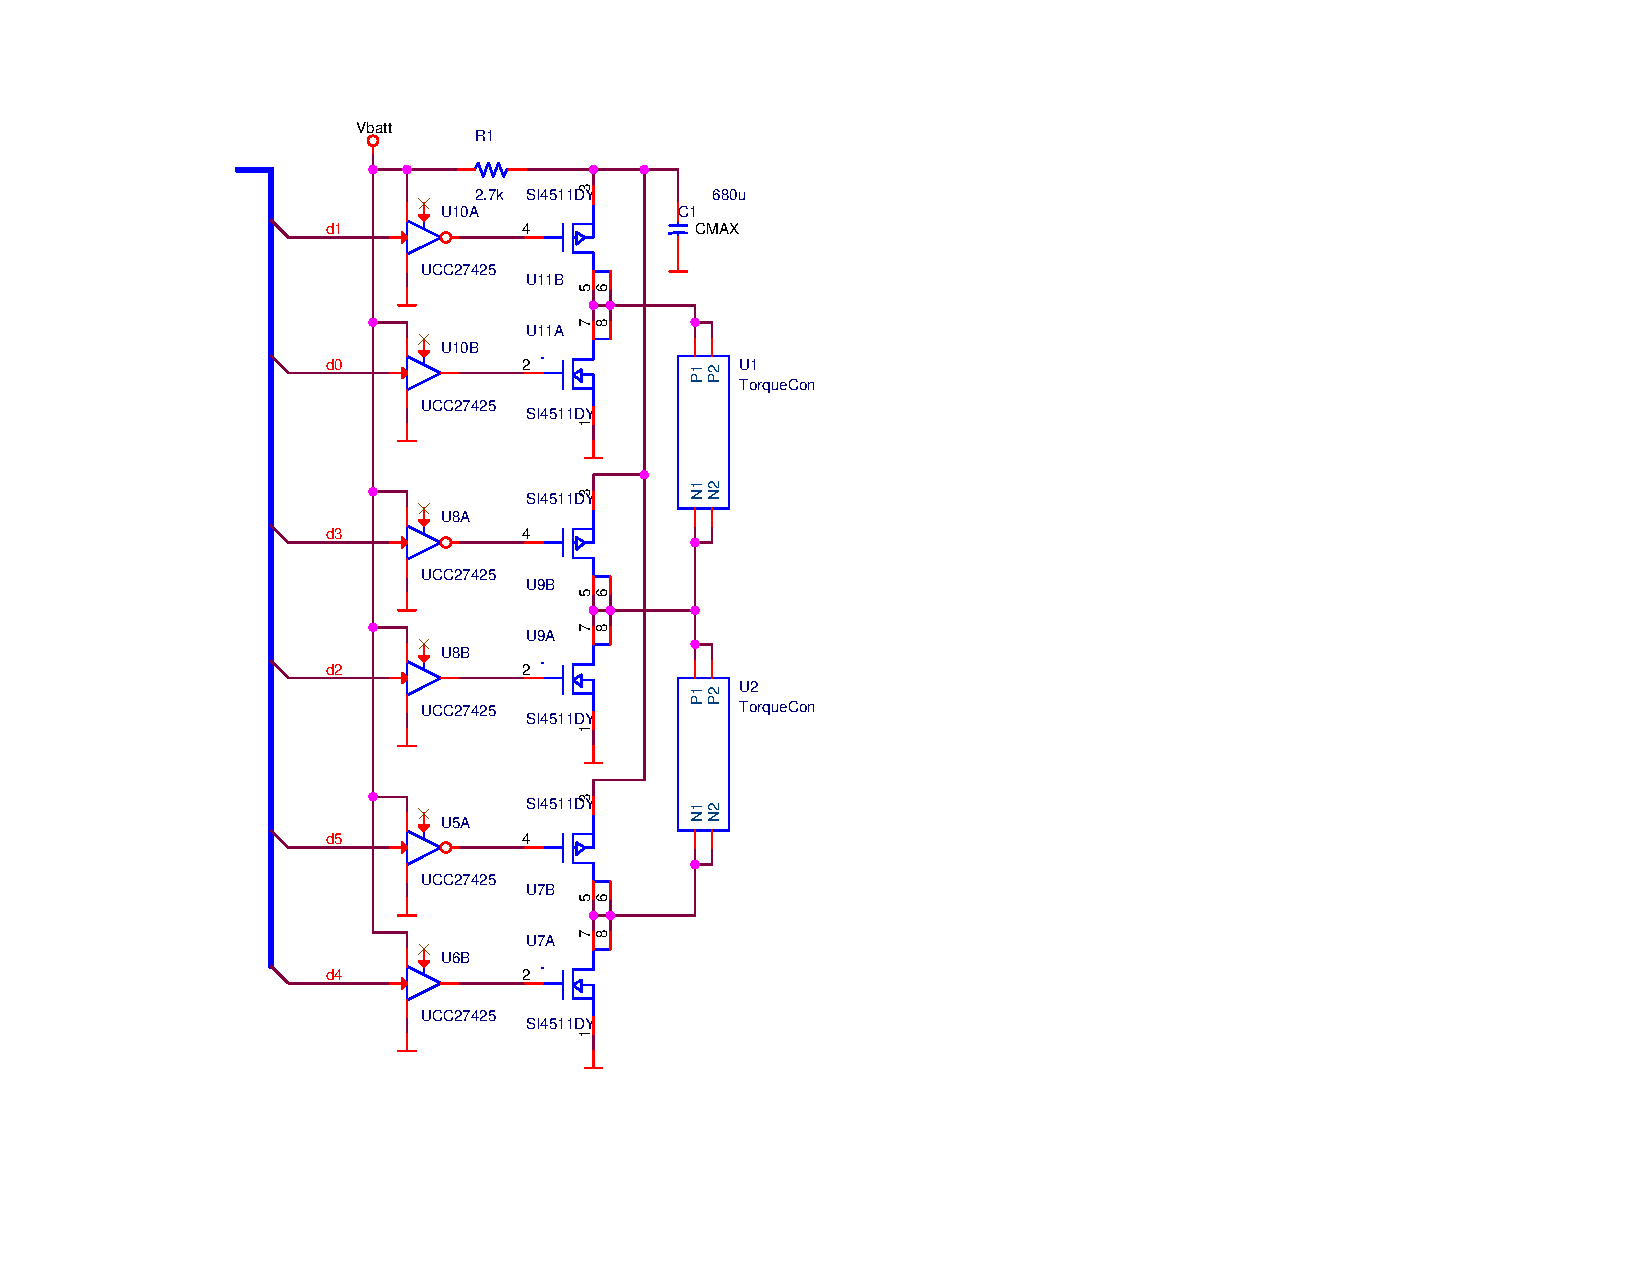
\includegraphics[height=0.5\textheight]{Figures/driverSchematic}
    \caption{Torquer driver schematic}
    \label{fig:drive}
\end{figure}

The schematic of the circuit used to drive a pair of torquers is shown in \cref{fig:drive}. Each pair of torquers is driven by three complimentary pairs of \acp{MOSFET}.  The \acp{MOSFET} are driven by three pairs of \ac{MOSFET} drivers that are controlled by the \ac{ACDS} microcontroller. The capacitor C1 is shared between both pairs of torquers in each axis giving a total of three capacitors on the \ac{ACDS} board. This means that only one torquer in each axis can be flipped each second. 

In the idle state, all of the \acp{MOSFET} are off and the torquer coils are floating. This prevents unwanted currents from flowing in the torquers. If \acp{MOSFET} are left on, providing a current path between the coil terminals, currents can be induced in the coils as the satellite turns and the magnetic field in the torquers changes. To flip a torquer, one end of the torquer is connected to ground using one of the N-Channel \acp{MOSFET} and the other end is connected to capacitor C1 using one of the P-Channel \acp{MOSFET}. After a 2 ms delay, the \acp{MOSFET} are switched off and C1 begins to recharge.

\subsubsection{Driving Waveform}

\begin{figure}[htb!]
    \centering
    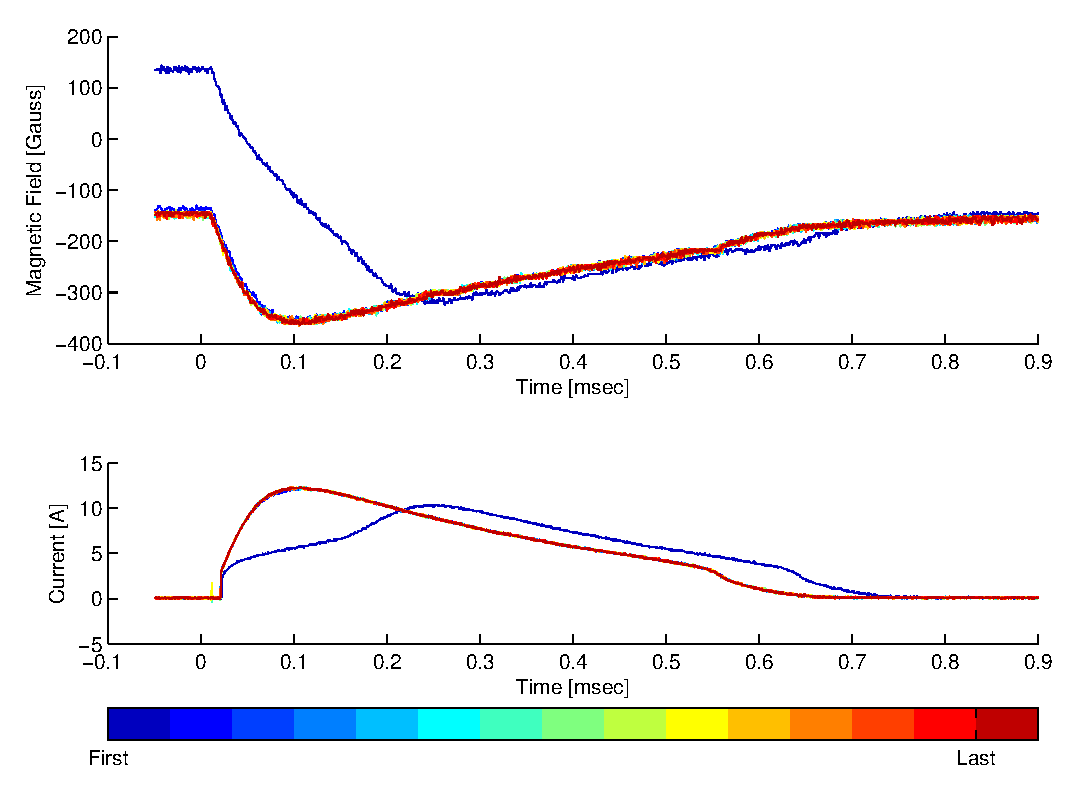
\includegraphics[width=\textwidth]{torquer-waveforms}
    \caption{Torquer driving waveform showing multiple torquer flips.}
    \label{fig:driveWV}
\end{figure}

\Cref{fig:driveWV} shows the driving waveform when driving a torquer multiple times in the same direction. The first torquer flip is shown in blue and the last flip is shown in red. The first waveform is the only waveform that differs significantly from the subsequent waveforms because the torquer is fully saturated in the first flip, thus demonstrating that the driving circuit is adequate to completely flip the torquers using a single 2~ms pulse.

The magnetic field waveform for the first flip starts at about +125~Gauss. This is because the torquer was flipped in the opposite direction before the test started. The subsequent waveforms start at about -125~Gauss. This is because the first flip drives the torquer into saturation flipping the torquers direction of magnetization. For all of the flips after the first flip, the change in magnetic field waveform is only due to the torquer coil and not to an actual torquer flip.

The current waveforms also show changes due to torquer saturation. For the first flip the current initially increases at a slower rate. This is because, on the Alnico1 B-H curve, the slope is steeper closer to the B-axis resulting in a higher inductance. As the torquer reaches saturation, the inductance of the torquer goes down and the rate of change of current increases. For the subsequent torquer flips, the torquer is already saturated so the inductance is low and the driving current reaches its peak much faster.

\begin{figure}[htb!]
    \centering
    \begin{tikzpicture}[remember picture,node distance=1em]
        \begin{pgfonlayer}{background}
            \node[anchor=south west,inner sep=0] (image) at (0,0) {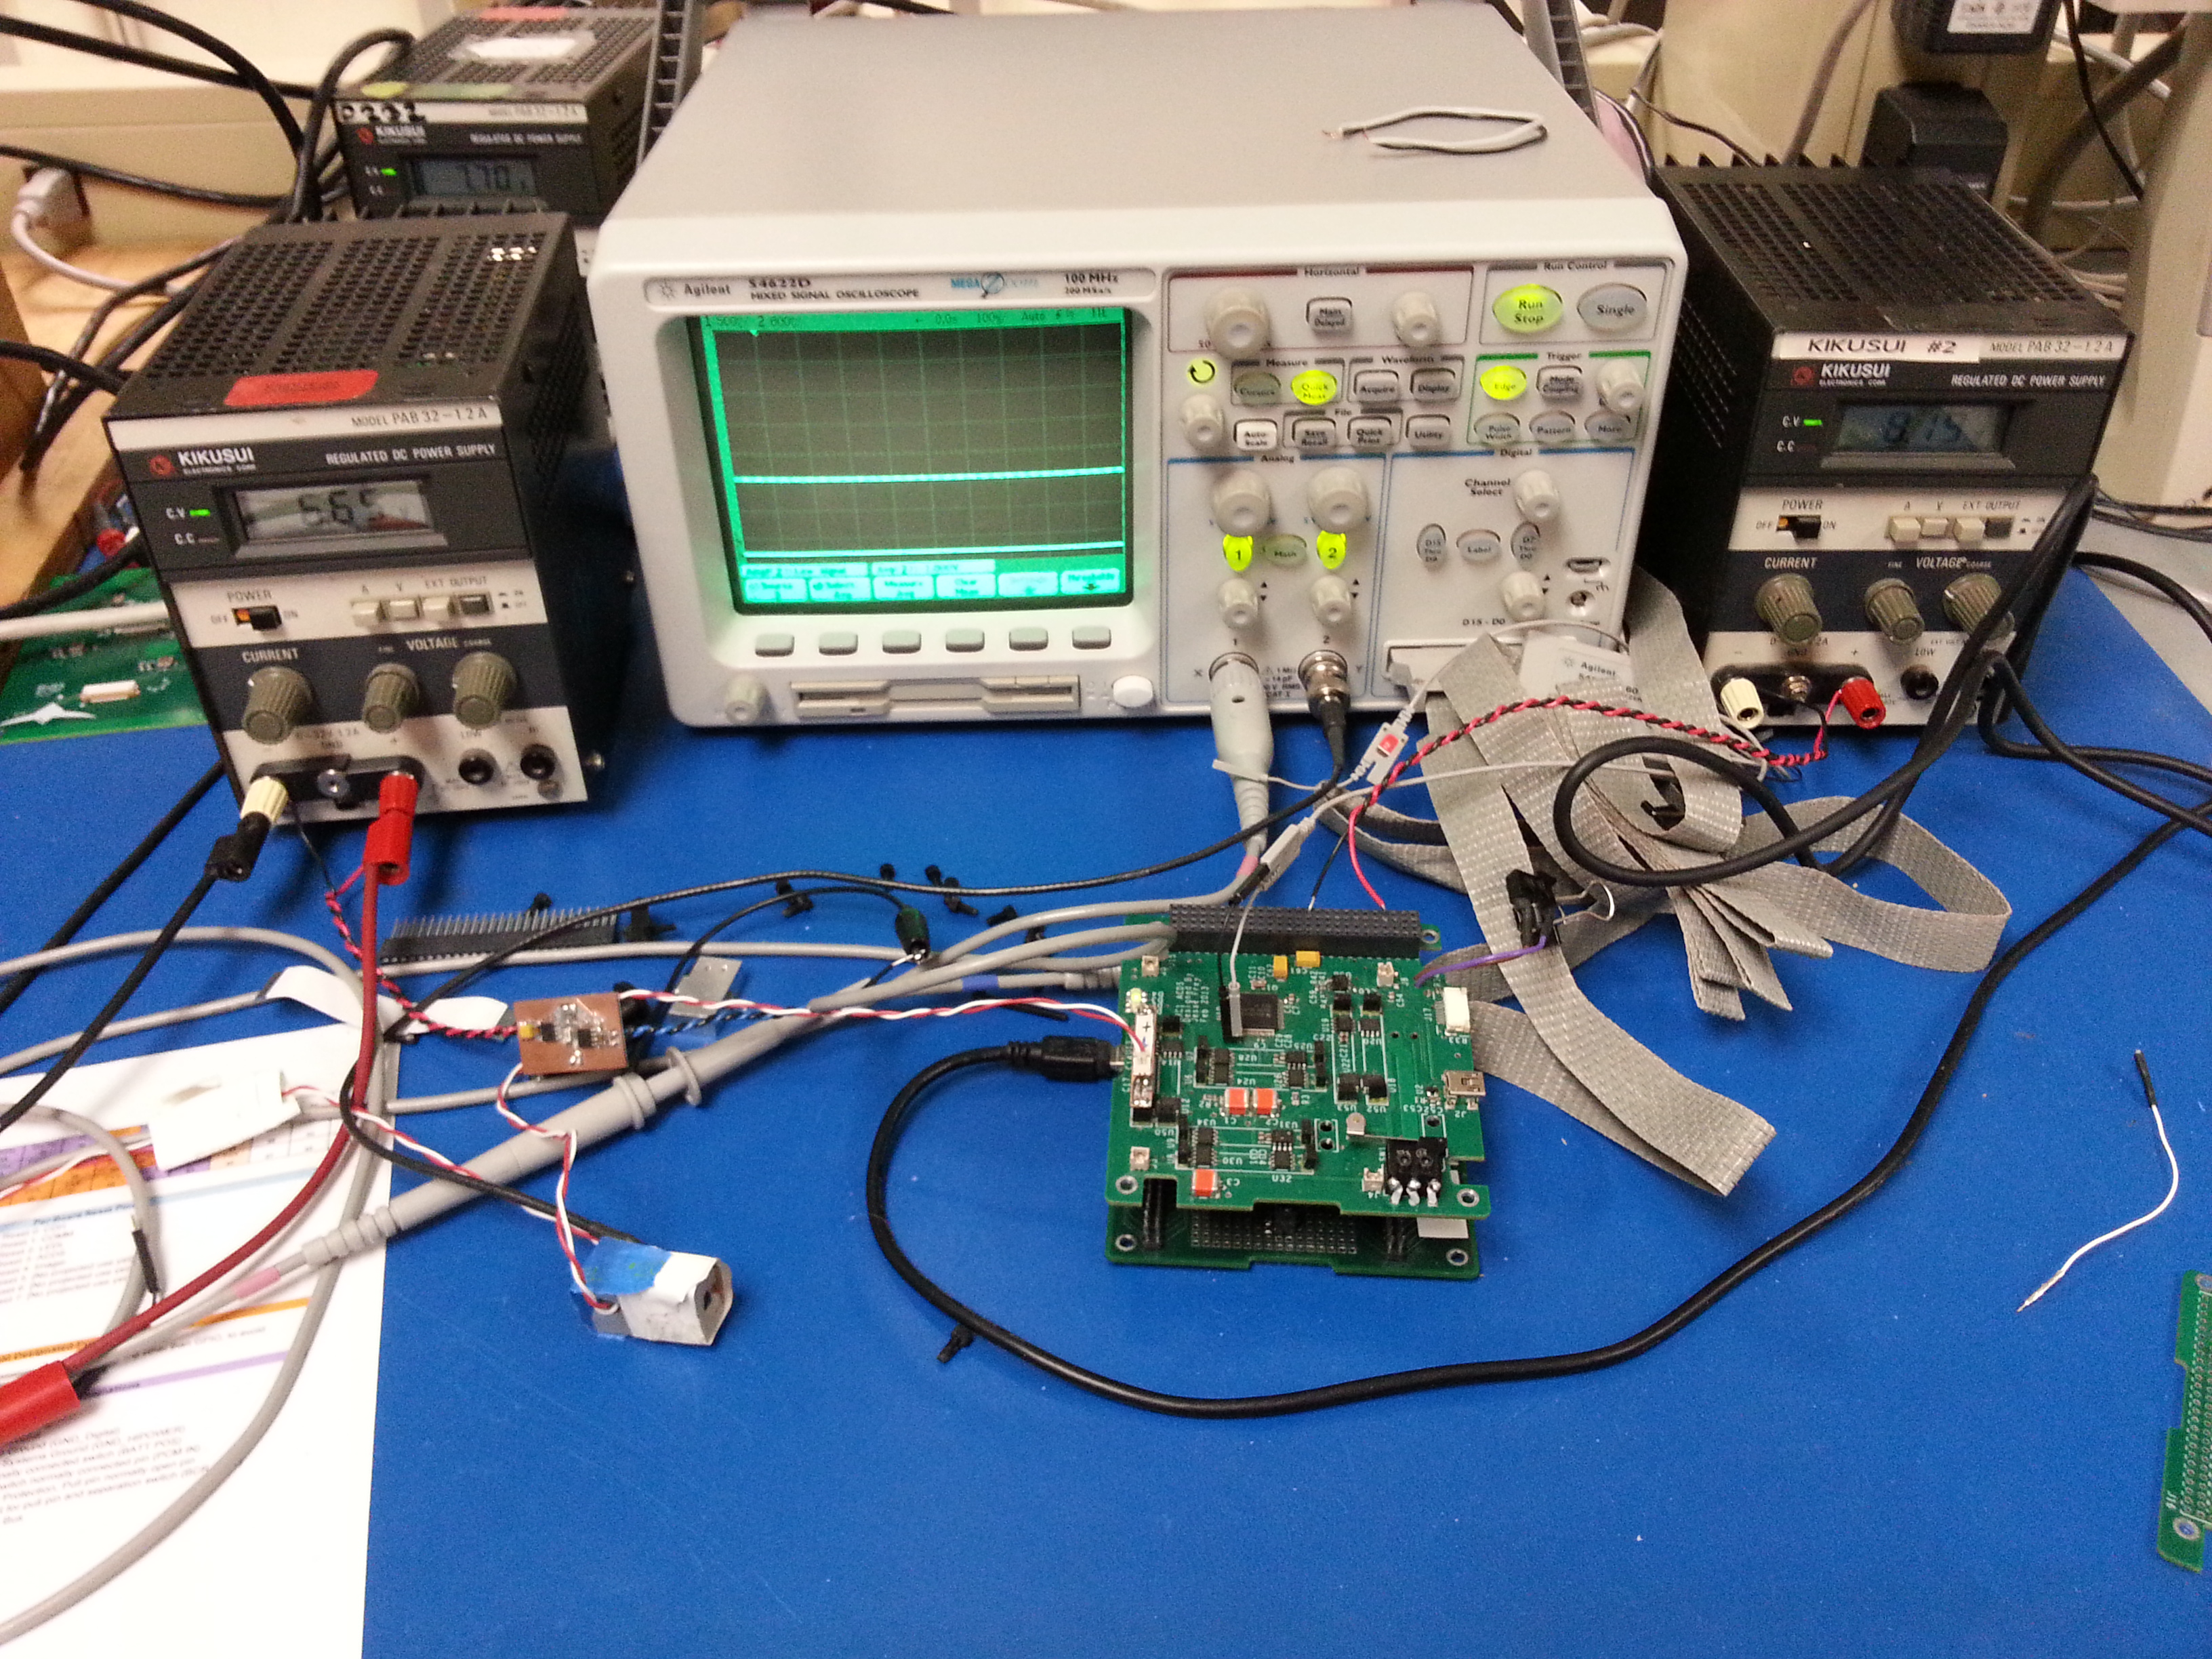
\includegraphics[width=\linewidth]{torquer-waveform-setup}};
        \end{pgfonlayer}
        %insert detail image
        \begin{scope}[x={(image.south east)},y={(image.north west)}]
            \node[inner sep=0] (detail) at (0.13,0.19) {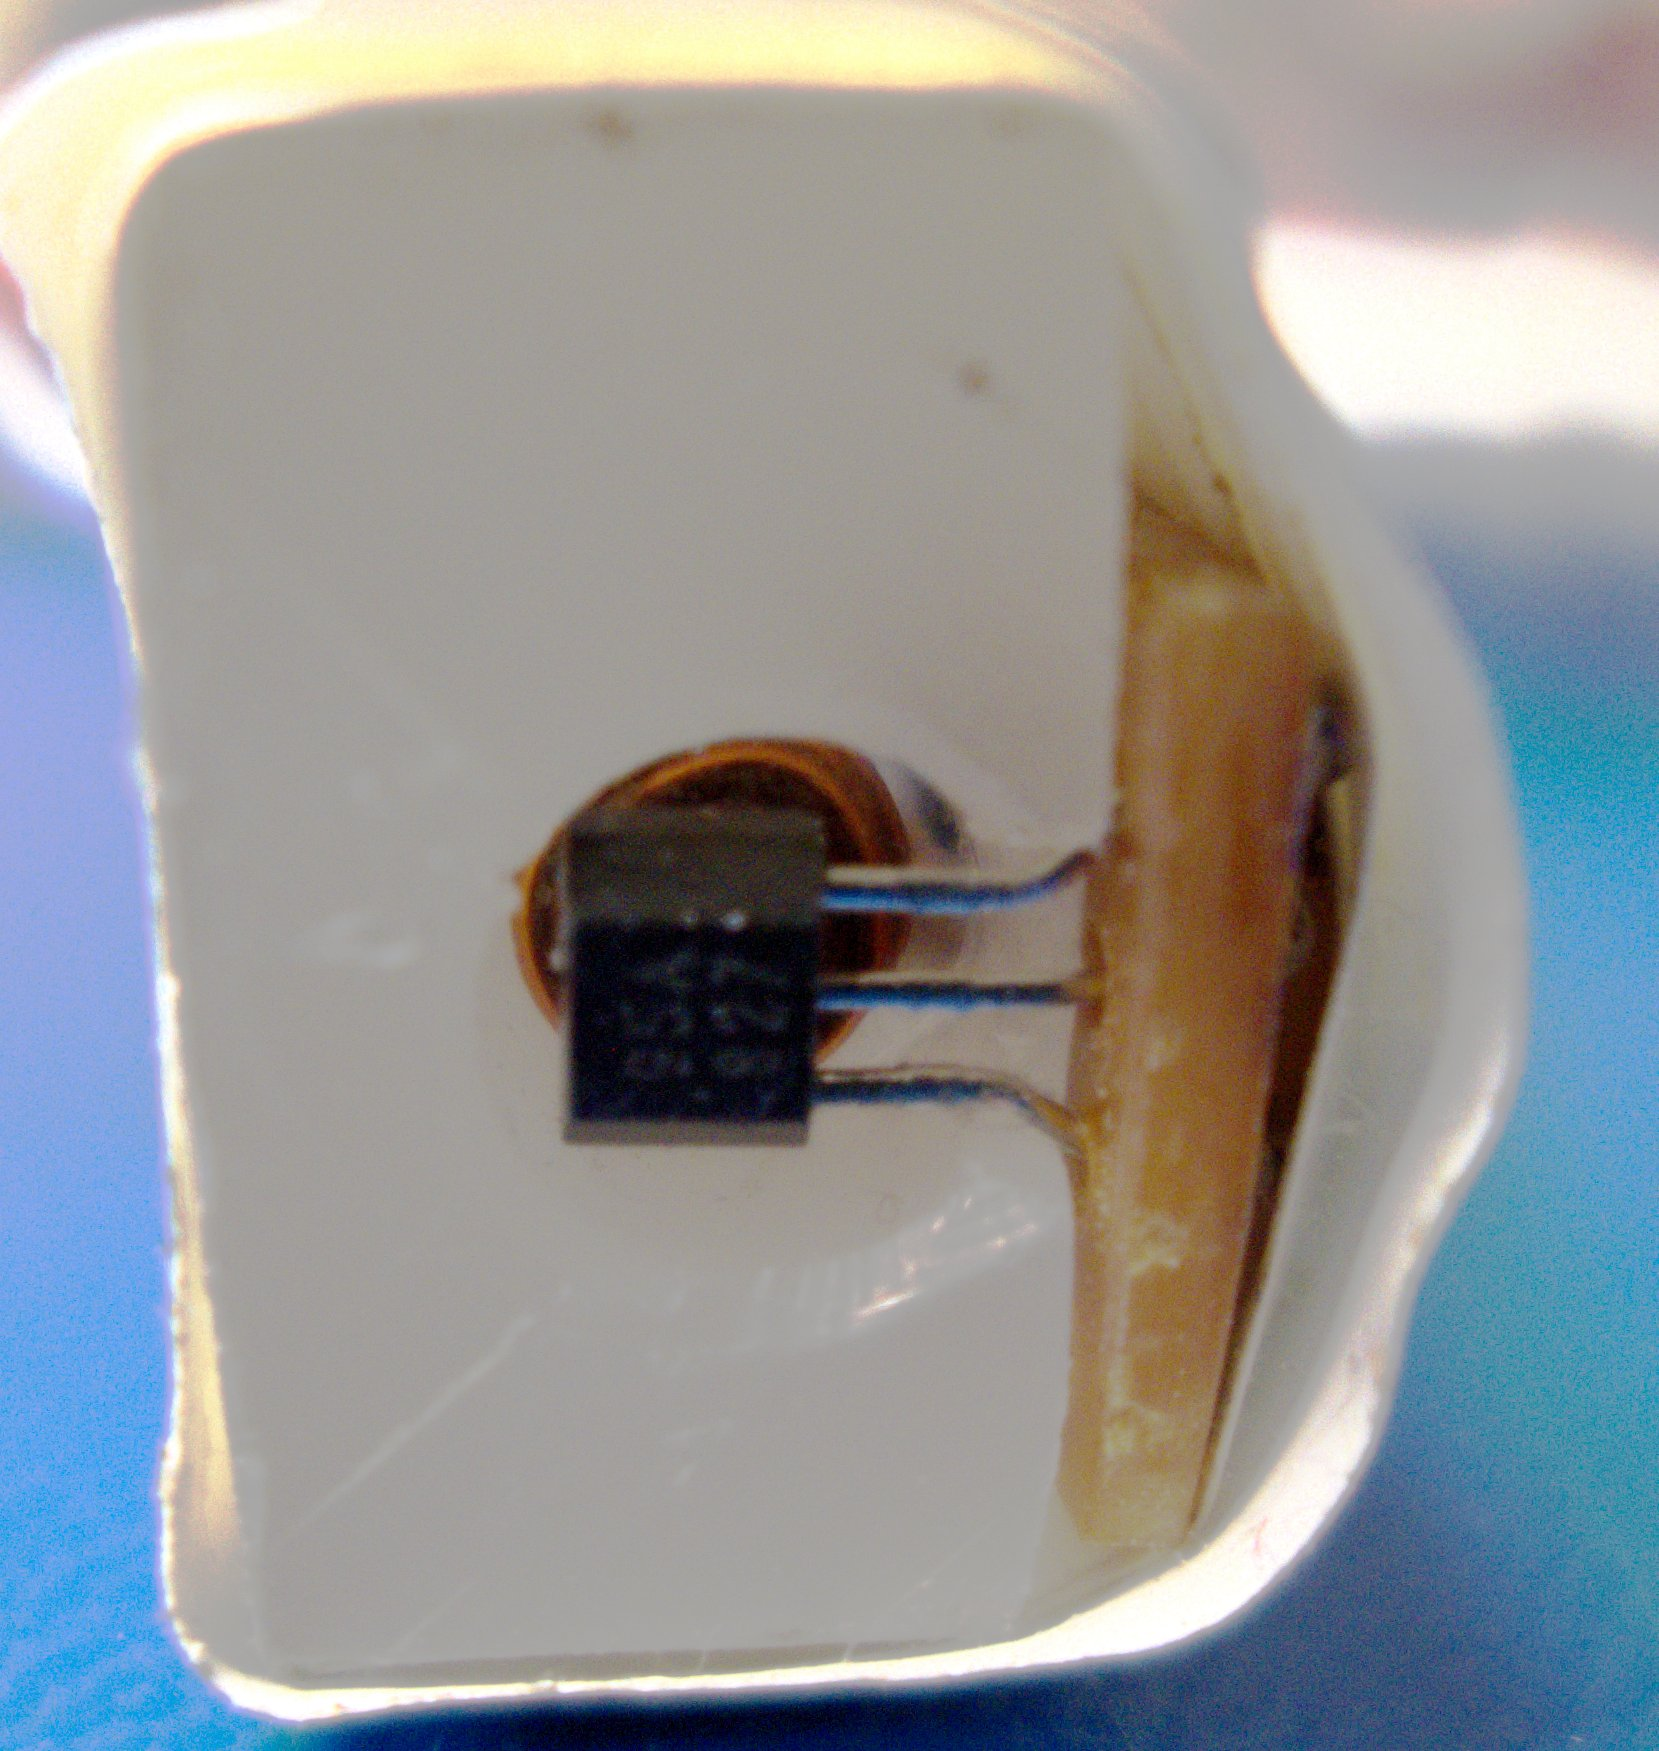
\includegraphics[width=1in,angle=-90]{testing-sensor}};
            %declare coordinates for box around sensor
            \path   (0.31,0.17) coordinate (box1)
                    (0.31,0.22) coordinate (box2)
                    (0.28,0.22) coordinate (box3)
                    (0.28,0.17) coordinate (box4);
            %draw box around sensor detail
            \draw[magenta,very thick] (detail.south east) -- (detail.south west) -- (detail.north west) -- (detail.north east) -- cycle;
            %draw box around sensor
            \draw[red,very thick] (box1) -- (box2) -- (box3) -- (box4) -- cycle;
            %draw "expanding lines" to detail
            \begin{pgfonlayer}{background}
                \draw[red,very thick] (box1) -- (detail.south east);
                \draw[red,very thick] (box2) -- (detail.north east);
                \draw[red,very thick] (box3) -- (detail.north west);
                \draw[red,very thick] (box4) -- (detail.south west);
            \end{pgfonlayer}
        \end{scope}
    \end{tikzpicture}
    \caption{Setup for measurements shown in \cref{fig:driveWV,fig:satWV}. The Hall effect sensor on the end of the torquer is shown in detail.}
    \label{fig:WVsetup}
\end{figure}

\Cref{fig:WVsetup} shows the hardware used to take the data for \cref{fig:driveWV,fig:satWV}. The \ac{ACDS} board was used to drive the torquers. To communicate with the \ac{ACDS}, another microcontroller board was used along with a \ac{USB}-to-serial converter. The torquer connects to the \ac{ACDS} board through a current sensor which is read by the oscilloscope. The torquer is placed inside a plastic housing with an attached Hall effect sensor to read the magnetic field. The Hall effect sensor is located against the end of the torquer and is read by the oscilloscope. A pin on the \ac{ACDS} microcontroller is  used to trigger the scope which is automatically configured by a \matlab script that communicates with the \ac{ACDS} board and the oscilloscope.

\begin{figure}[htb!]
    \centering
    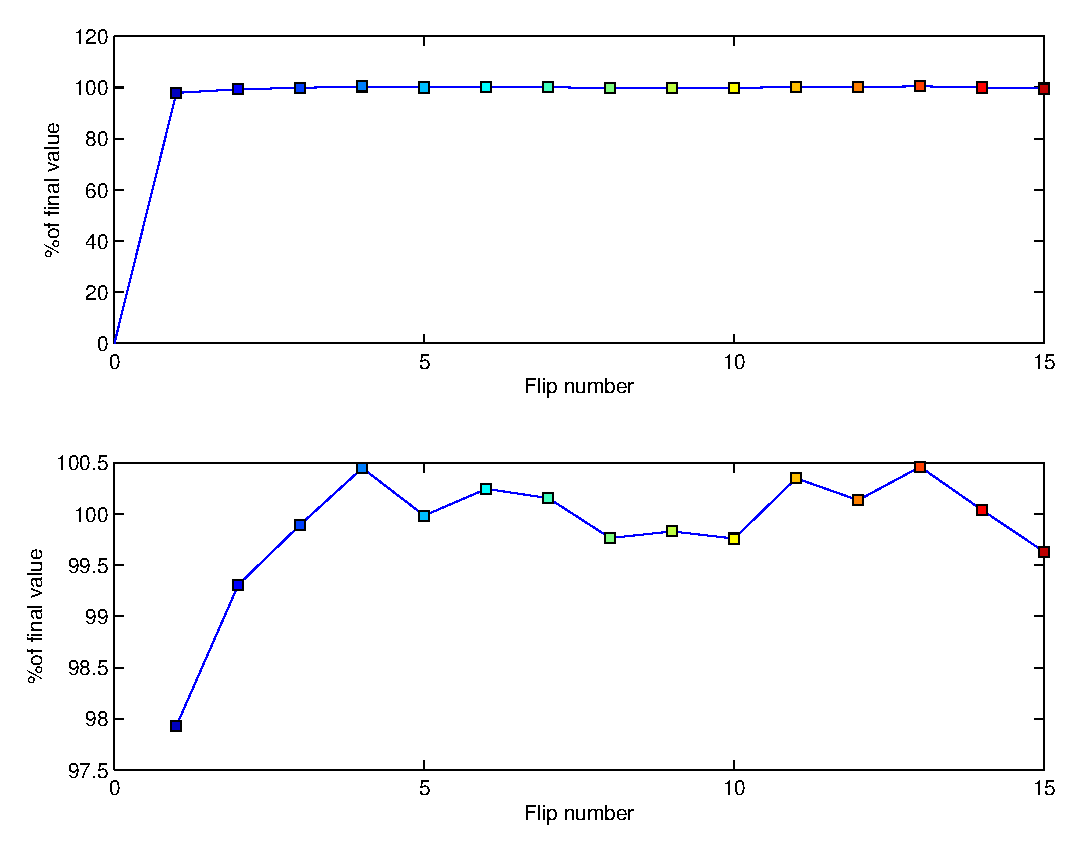
\includegraphics[width=\textwidth]{torquer-multiflip}
    \caption{Torquer saturation}
    \label{fig:satWV}
\end{figure}

%TODO: fix this sentance

The measured field that the Hall effect sensor reads is highly dependant on the distance from the torquer. The residual induction of Alnico1 is 7200 Gauss \cite{AlnicoProp}. For the radius ($\sfrac{1}{32}~\unit{inch}$) and length of the torquer (1~inch), the calculated magnetic field of the torquers is 155~Gauss at 0.05~in from the face of the torquer in the torquer axis\cite{DexterField}. This is close to what is shown in \cref{fig:driveWV}. As the distance from the face increases to 0.1,~0.2~and~0.3~inches the field decreases to 46,~12~and~5~Gauss, respectively.

\Cref{fig:satWV} shows how the torquer field changes as the number of flips increases. Both graphs show the same data, with the lower graph zoomed in to better show the points after the first flip. The 0\% point is found by averaging 20 samples from the beginning of the first magnetic field waveform in \cref{fig:driveWV}. The rest of the points are found by averaging the last 20 samples of the magnetic field waveforms from \cref{fig:driveWV}. The first flip gets the torquer field to within 97\% of the final value and after two flips it has reached the final value. 

\subsection{Torquer Diagnostics}

\begin{figure}[htb!]
    \centering
    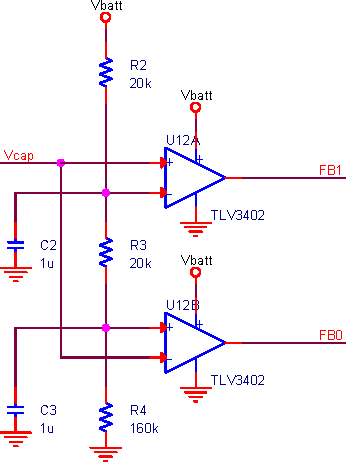
\includegraphics{fb-comp}
    \caption{Torquer feedback comparators}
    \label{fig:fb-comp}
\end{figure}

\Cref{fig:fb-comp} shows the torquer feedback comparators that are used to detect if the torquers and drivers are functioning properly in flight. Vcap is the voltage from capacitor C1 in \cref{fig:drive}. The comparator outputs, FB0 and FB1, have open drain outputs that are pulled up to logic hi by internal resistors on the MSP430 inputs. U12A  is used to determine if the capacitor is charged and U12B is used to detect if the capacitor is discharged. The comparators are checked both before and after a torquer flip to see if the capacitor was charged before an attempted flip and discharged after. If the capacitor did not discharge, then the torquer did not flip, probably because of a bad connection or failed component somewhere. This information is logged in flight and can be downlinked to analyze if the torquers are firing correctly.

\section{Sensors}

The only sensor specified in \cite{Mentch11} was a magnetometer. The magnetometer was proposed to be used to determine the angular rates of the \ac{ARC} as well as an input to \cref{eq:crossl}. Because the torque produced by the torquers depends on the Earth's magnetic field, the Earth's magnetic field must be known in order for the algorithm to compute the necessary dipole moment. The accuracy of the magnetometer was not specified but it needs to be able to determine rotation rates accurately enough for the \ac{ACDS} to work.

\subsection{Magnetometer}

The magnetometers on the satellite are Honeywell HMC1052 \ac{AMR} sensors. These sensors use \ac{AMR} elements in a bridge configuration to measure the field in each axis. The HMC1052 is a 2-axis sensor that measures the field in the axis that are parallel to the board that it is mounted on (X and Y). Each face of \ac{ARC} will have a single HMC1052 giving a total of 4 measurements in each axis.

The magnetometers are located on the back of the \acs{SPB}, shown in \cref{fig:SPB}. The magnetometer, with surrounding circuitry, is visible on the back of the board as are the \ac{ADC} and amplifier. An accelerometer is also located on the back of the solar panel board and is used for a different mission objective. The data connector powers the sensors and provides access to the sensor data.

\subsubsection{Magnetometer Amplifier}

The \ac{SPB} also contains an amplifier to amplify the magnetometer signal before it is read by the \ac{ADC}. This allows the output voltage of the magnetometer to fill the input range of the \ac{ADC}. The required range of the magnetometer will be largely dependent on the torquer geometry and could be more than the \textpm 600~mGauss or so of Earth's field. The amplifier can be used to trade range for resolution depending on requirements.

\Cref{eq:amp-gain} shows the equation used to calculate the desired amplifier gain. The maximum voltage readable by the \ac{ADC}, $V_{adc}$, is divided by the maximum expected output from the magnetometer. The maximum output from the magnetometer is found by adding the output due to the desired full scale field and the maximum possible bridge offset.

\begin{equation}
    \label{eq:amp-gain}
    A = \frac{V_{adc}}{B_{max} \cdot V_{bridge} \cdot S_s + V_{os} \cdot V_{bridge}}
\end{equation}

\Cref{eq:amp-gain-calc} shows the gain calculations for the magnetometer amplifier to measure a \textpm 4~Gauss field. The bridge and \ac{ADC} reference voltages are 3.3~V. This gives an input voltage range for the \ac{ADC} of \textpm 1.65~V.

\begin{equation}
    \label{eq:amp-gain-calc}
    \begin{split}
        A &= \frac{1.65~\unit{V}}{4~\unit{Gauss} \cdot 3.3~\unit{V} \cdot 1~\unit{mV/V/Gauss} + 1.25~\unit{mV/V} \cdot 3.3~\unit{V}}\\ 
          &= \frac{1.65~\unit{V}}{13.2~\unit{mV} + 4.125~\unit{mV}} \\
          &= \frac{1.65~\unit{V}}{17.325~\unit{mV}} \\
          &= 95.24
    \end{split}
\end{equation}


\subsubsection{Magnetometer \acl*{ADC}}

Each magnetometer has its own \ac{ADC} on each \ac{SPB}. The \ac{ADC} used is the LTC2487. The LTC2487 is a 16-bit delta sigma \ac{ADC} that has two differential analog input channels and an \ac{I2C} interface. For a bridge voltage of 3.3~V, the HMC1052 has a sensitivity 3.3~mV/Gauss. If the amplifier gain is 95 this results in a sensitivity of 0.31~V/Gauss. For a 3.3~V reference voltage, the \ac{ADC} has a resolution of $25~\unit{\mu V}$, which results in a resolution of $81~\unit{\mu Gauss}$ / LSB.

\subsubsection{Magnetometer Operation}
%\subsection{\acs*{AMR} Background}

The HMC1052 sensors used on the \ac{ACDS} are \ac{AMR} sensors. They work by having a bridge with 4 elements that all change resistance with the applied magnetic field. The \ac{AMR} sensors are primarily sensitive to magnetic fields in their sensitive direction, ($H_s$), but they are also slightly sensitive to magnetic fields in an axis normal to the sensitive direction, ($H_C$), called the cross axis. The sensor is only sensitive to magnetic fields that are in the film plane of the \ac{AMR} sensor. For the 2-axis HMC1052 this means that both sensors show some sensitivity to fields in both the X and Y axes as shown in \cref{fig:magAxisCross}. The cross axis effect varies from sensor to sensor so calibration values must be calculated for each sensor \cite{AN215}.

\begin{figure}[H]
    \centering
    \begin{tikzpicture}[scale=2]
        \def\L{0.5}     %define arrow length
        \def\W{0.3}     %define arrow length
        \draw[fill=black] (\W,\W) rectangle (-\W,-\W);
        \draw[->,red,>=stealth,thick] (0  , 0) -- (\L,0);
        \draw (\L,0) node[anchor=west] {$H_c$};
        \draw[->,red,>=stealth,thick] (0, 0) -- (0,\L);
        \draw (0,\L) node[anchor=south] {$H_s$};
    \end{tikzpicture}
    \caption{Magnetometer showing $H_s$ and $H_c$}
    \label{fig:magAxisCross}
\end{figure}

\Cref{eq:magcross} shows the simplified equation for the magnetometer as described in \cite{AN215}. $V_b$ is the bridge voltage that is applied to the sensor. $S_s$ is the sensitivity in the sensitive direction. D is the cross field sensitivity offset. The HMC1052 datasheet\cite{HMC1052} mentions that the sensors have a bridge offset. The bridge offset is the sensor output when zero field is applied to the sensor and can be as large as \textpm1.25 Gauss. The bridge represented by $V_{os}$ in \cref{eq:magcross}.

\begin{equation}
    V_s = V_b \left(S_s H_s + D \cdot H_c + V_{os} \right)
    \label{eq:magcross}
\end{equation}
 
The bridge voltages are measured using an \ac{ADC} that uses the bridge voltage as its reference. To take this into account and simplify the equations, the following substitution is made:
\begin{equation}
    V_s'=\frac{V_s}{V_b}
    \label{eq:adcsub}
\end{equation}

\Cref{eq:magcross} is useful to determine the voltage that would be produced for a given magnetic field condition, but not the reverse when the sensor voltages are known but the fields are not.

Because the calculated field in the sensitive direction also depends on the field in the cross axis direction, \cref{eq:magcross} was duplicated for the cross field sensor voltage and both equations were solved simultaneously. This resulted in twice as many constants as \cref{eq:magcross}. The voltages $V_s'$ and $V_c'$ are the normalized \ac{ADC} voltages in the sensitive and cross axes, respectively. Each of the constants from \cref{eq:magcross} has similar duplicate forms that comes from the extra equation that was used to solve for $H_s$. To distinguish the constants additional subscripts have been added. For example ${S_s}_s$ is the sensistivity of the sensitive axis field to the sensitive axis input while ${S_s}_c$ is the sensitivity of the cross axis to magnetic fields in the sensitive axis direction. \Cref{eq:magsolved} shows \cref{eq:magcross} solved for the unknown quantity, $H_s$.

\begin{equation}
    \begin{split}
    H_s = & \frac{V'_s }{{S_s}_s - \frac{D_s \cdot D_c}{{S_s}_c}} - \frac{D_s \cdot  V'_c }{{S_s}_c \cdot {S_s}_s - D_s \cdot D_c}\\
    & {}- \frac{{S_s}_c \cdot {V_{os}}_s  -D_s \cdot {V_{os}}_c}{{S_s}_c \cdot {S_s}_s - D_s \cdot D_c}
    \end{split}
    \label{eq:magsolved} 
\end{equation}

\Cref{eq:magsolved} can be used to calculate the magnetic field from measured voltages, but the relationship between the constants is complex. To simplify \cref{eq:magsolved} the constants can be consolidated, as shown in \cref{ch:mag-deriv}, to get \cref{eq:magcal}.

\begin{equation}
    \label{eq:magcal}
    \begin{split}
        H_s &= C_1 \cdot V_s' + C_2 \cdot V_c' + C_3\\
        H_c &= C_4 \cdot V_s' + C_5 \cdot V_c' + C_6
    \end{split}
\end{equation}

In this case $V_s'$ and $V_c'$ are the \ac{ADC} values for the sensitive and cross axes, respectively. $C_1$, $C_2$, $C_4$, and $C_5$ are the sensitivity in the sensitive and cross directions and $C_3$ and $C_6$ correct for the bridge offset of the sensor and also compensates for external offsets. These offset values are used to correct for the torquer offsets.

\subsubsection{Magnetometer Calibration}
\label{sec:magcal}

To calibrate the magnetometer, the coefficients in \cref{eq:magcal} must be calculated. The magnetometer is first placed inside the Helmholtz Cage. The field is set under \matlab control so the entire calibration process can run automatically. The calibration program sweeps the field inside the Helmholtz Cage through a predefined sequence and reads the sensor output at each point. 

The method of least squares is used to solve \cref{eq:magmat} for the coefficients in \cref{eq:magcal}. Each line in the $\matt{A}$ matrix represents a separate magnetic field measurement. $H_n$ is the $n^{\text{\tiny th}}$ value set by the Helmholtz cage in the sensitive axis. 

\begin{equation}
    \label{eq:magmat}
    \begin{split}
    \vect{b}&=\matt{A} \vect{x} \\
    {\text{\raggedright where}} \\
    \vect{b}&= 
    \begin{bmatrix}
        H_1 \\
        \vdots \\
        H_n \\
    \end{bmatrix} \\
    \matt{A}&=
    \begin{bmatrix}
        {V_s}_1 & {V_c}_1 & 1 \\
        \vdots & \vdots & \vdots\\
        {V_s}_n & {V_c}_n & 1 \\
    \end{bmatrix} \\
    \vect{x}&= 
    \begin{bmatrix}
        C_1 \\
        C_2 \\
        C_3 \\
    \end{bmatrix} 
    \end{split}
\end{equation}

The least squared solution minimizes the error across all data points. This results in calibration values that minimize error across the range of calibration points that were taken. This means that the points used to do the calibration should span the range of values that the magnetometer is expected to measure. 

\subsection{\acs*{MEMS} Gyros}

For flight, a LPY410AL \ac{MEMS} gyro will also be used to sense rotation rates. \ac{MEMS} gyros have limited resolution compared to what can be achieved with the magnetometer. The LPY410AL has a maximum range of \textpm 400\textdegree /sec. The LPY410AL has a zero-rate sensitivity drift of 0.03~dps/\textdegree C. The desired rotation rate of the satellite is about 500~\textmu dps. This means that for a 1\textdegree C temperature change the rotation rate could change by 58 times the desired rotation rate. The LPY410AL also has a rate noise density of 0.014~$\unit{dps}{/}\sqrt{\unit{Hz}}$ so even at a slow sample rate of 1~Hz, the noise is 27,000 times larger than the desired rotation rate.

\ac{MEMS} gyros do, however, give good results if the rotation rates are large, such as after the satellite is ejected from the \ac{PPOD}. If the satellite is rotating fast enough, the magnetometer readings will alias and it can appear that the satellite is rotating at a speed that is much less than the actual speed. If the rotation rates are too high for the \ac{MEMS} gyro, the output will saturate, and while the rotation rates are not measurable, a direction and lower bound can be determined.


\section{Embedded System}

At the heart of the \ac{ACDS} is an embedded system. This system is responsible for running the algorithm, taking housekeeping data and, interfacing with the rest of the satellite.

\subsection{Processor}

The processor used for the \ac{ACDS} and all systems on \ac{ARC} is the Texas Instruments MSP430F2618. The MSP430 is a microcontroller aimed at low power applications. The MSP430f2618 runs at a maximum speed of 16~MHz and has 8~kB of \ac{RAM} and 116~kB of flash~memory. The MSP430 microcontrollers do not have an external memory bus so there is no way to add extra \ac{RAM} or flash~memory to the address space of the MSP430.

\subsection{SD card}

For flight data storage a SD card is used. This is necessary because of the needed space and write times. The internal flash is limited and also needs to be used for program storage making it undesirable for data storage. Furthermore, the internal flash can't be read while it is being written. Write times for the internal flash are fairly slow and require that the processor disable interrupts, making normal operation difficult. The flash shares the same address space as the \ac{RAM} and has the same access time. This makes the internal flash an attractive place to put settings and calibration data that are written few times but accessed often as any data on the SD card must be copied into \ac{RAM} before being used.

\subsection{\acs*{ARC} Bus Communication}

The sensor data is read by the \ac{LEDL} board and sent over the bus to the \ac{ACDS} board. The \ac{ACDS} board initiates the connection by sending a command to tell how often measurements should be sent. The \ac{LEDL} then takes sensor data and sends it at the requested interval.

\begin{comment}
\section{Finished Board}

\Cref{fig:boardPhoto} shows the finished \ac{ACDS} board with torquers and pull pin. 

\begin{figure}[!ht]
    \centering
    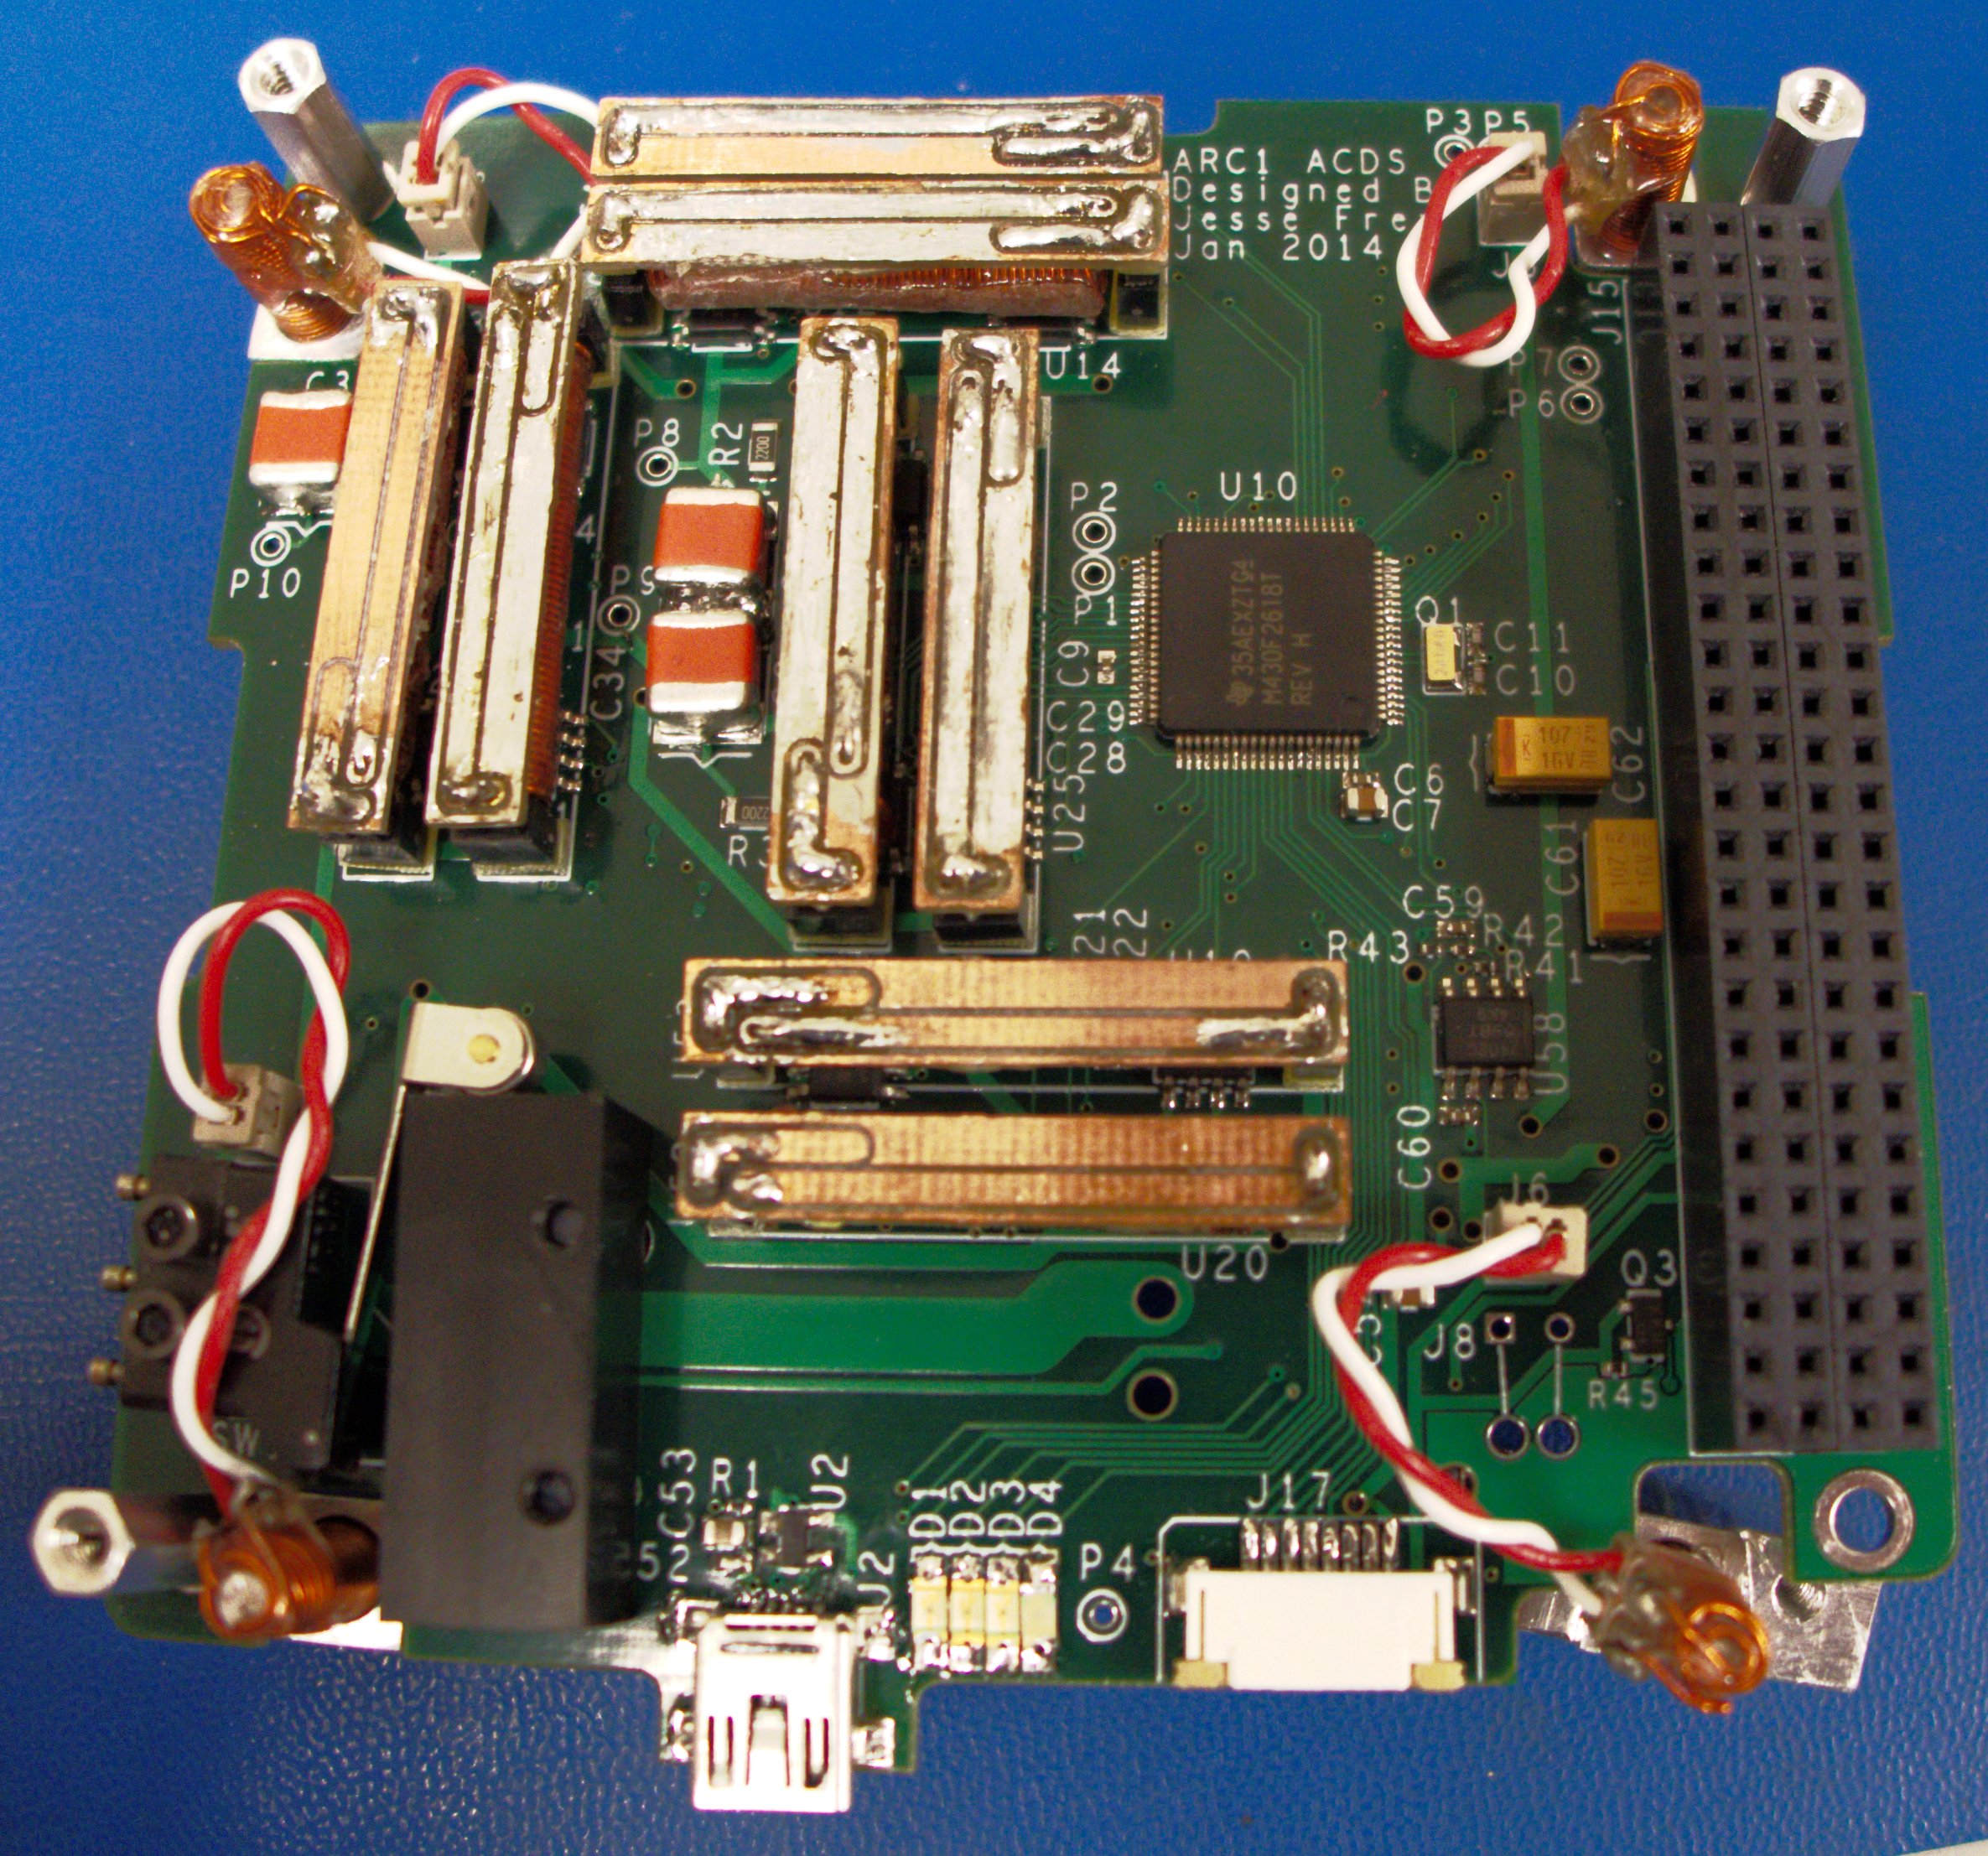
\includegraphics[width=0.5\linewidth]{ACDS-board-photo}
    \caption{The finished \ac{ARC} \ac{ACDS} hardware}
    \label{fig:boardPhoto}
\end{figure}
\end{comment}

\begin{comment}
\section{Board Layout}

\Cref{fig:3dview} shows the \ac{ACDS} system. The X and Y axis torquers are shown on the board as well as the pull pin and header. The header and pull pin locations are more or less fixed which doesn't leave much wiggle room for where to place the torquers.

\begin{figure}[H]
    \centering
    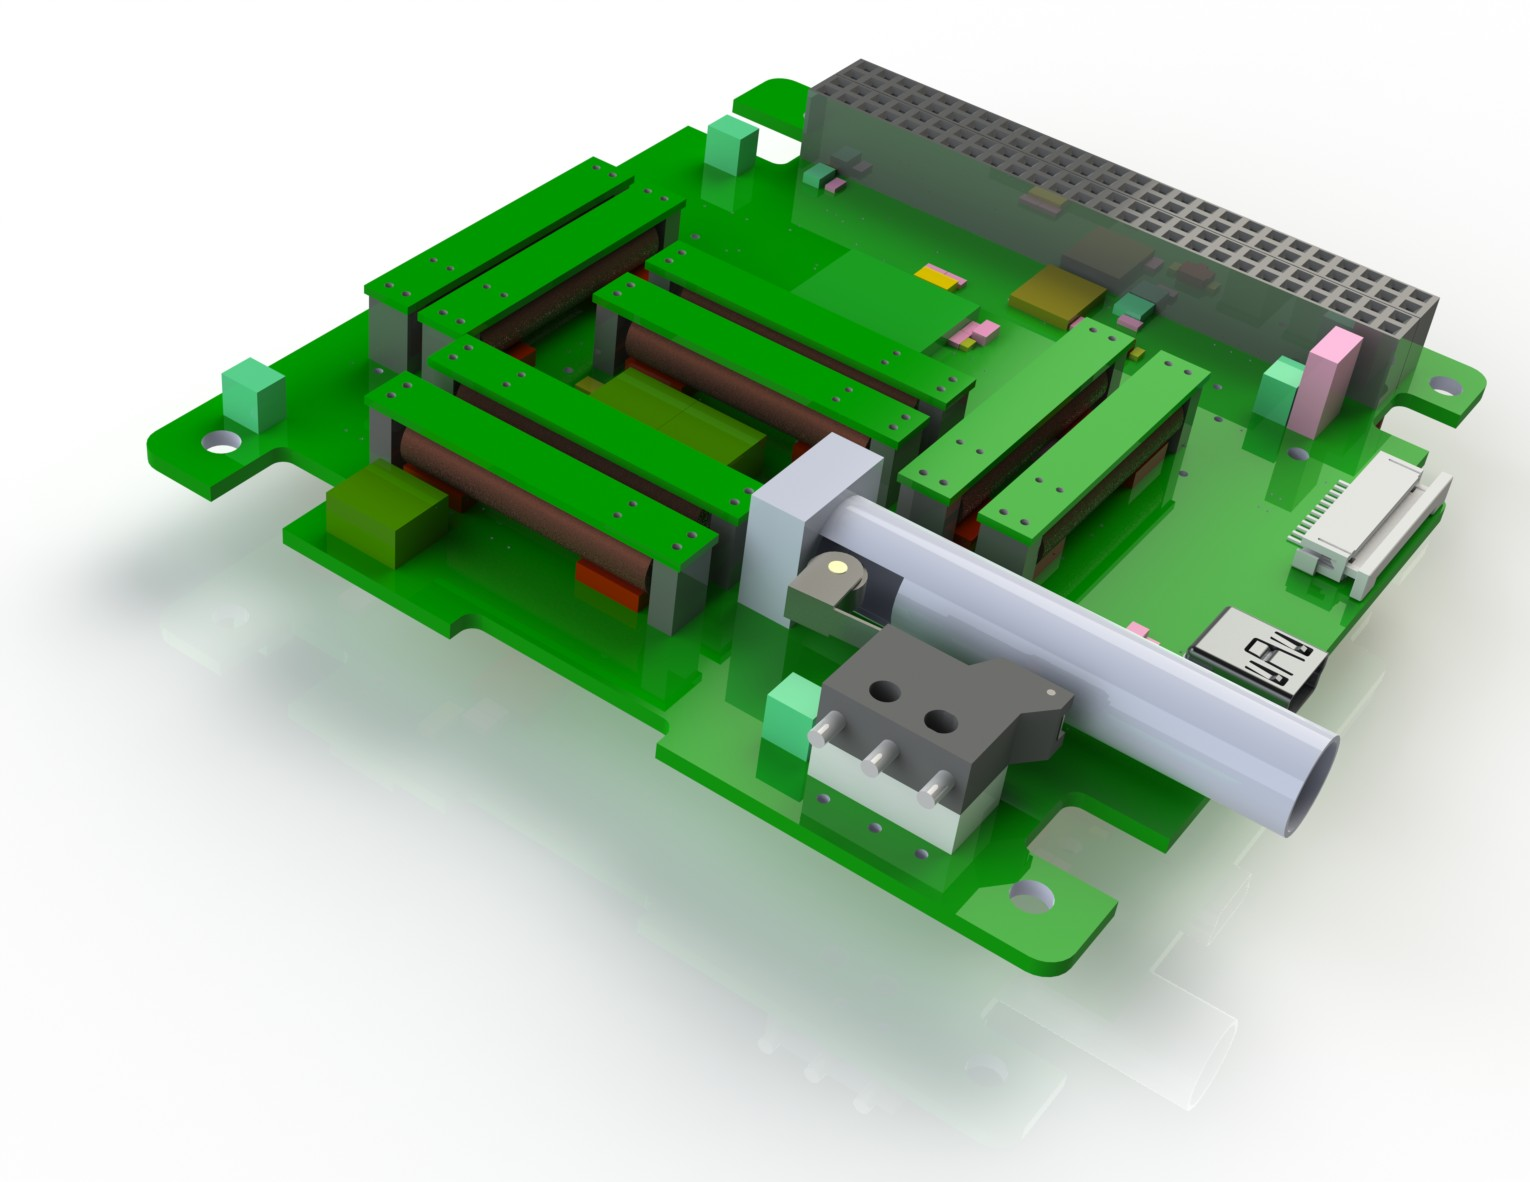
\includegraphics[width=\textwidth]{board-drawing}
    \caption{3D view of the CubeSat \acs*{ACDS} system}
    \label{fig:3dview}
\end{figure}

\end{comment}

\begin{comment}
\begin{figure}[H]
    \centering
    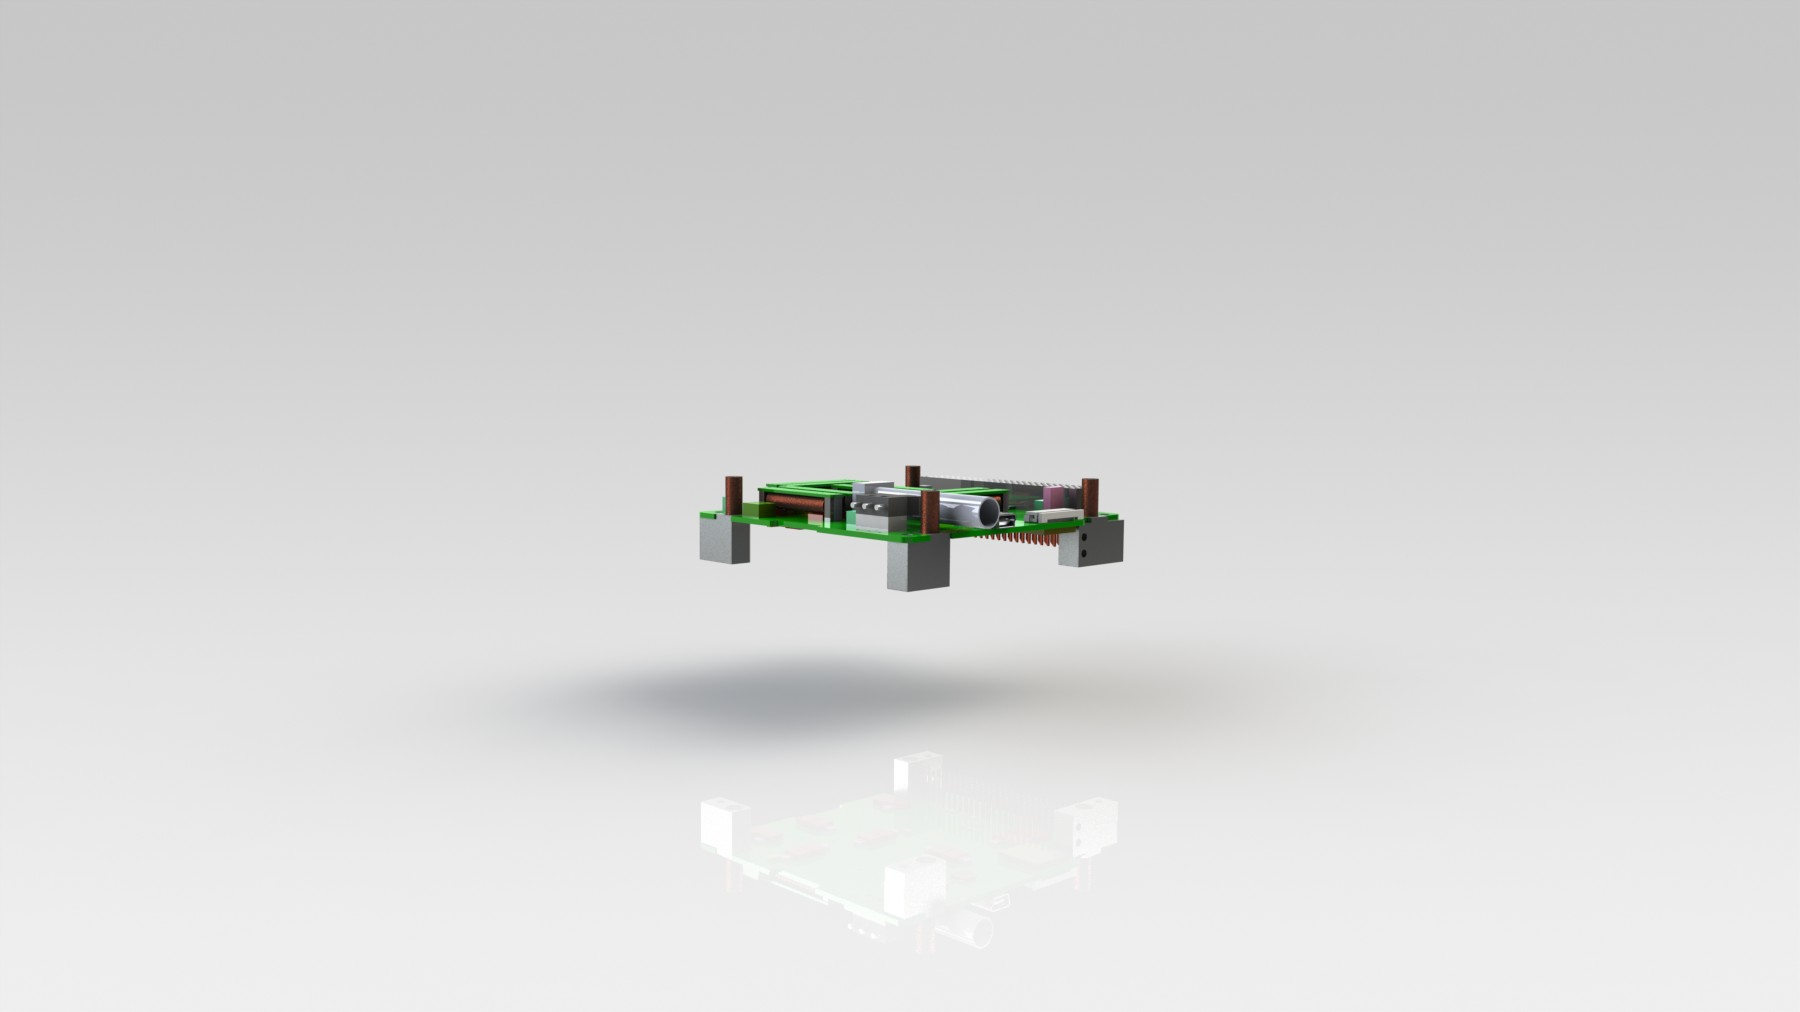
\includegraphics[width=\textwidth]{board-drawing-with-standoffs}
    \caption{3D view of the CubeSat \acs*{ACDS} system with Z-axis torquers}
\end{figure}
\end{comment}

\begin{comment}

The \ac{ACDS} board is a four layer board with the inner layers as power and ground planes. \Cref{fig:layout} shows the \ac{PCB} layout for the \ac{ACDS} board. The circuitry is very repetitive and this was used when the board was laid out. A quick switching time is desired and moderate currents are involved, the lines to and from the \acp{MOSFET} were kept as short as possible. The power plane is split so that there is a 3.3V plane underneath the MSP430 and a $V_{batt}$ plane elsewhere.

\begin{figure}[H]
    \centering
    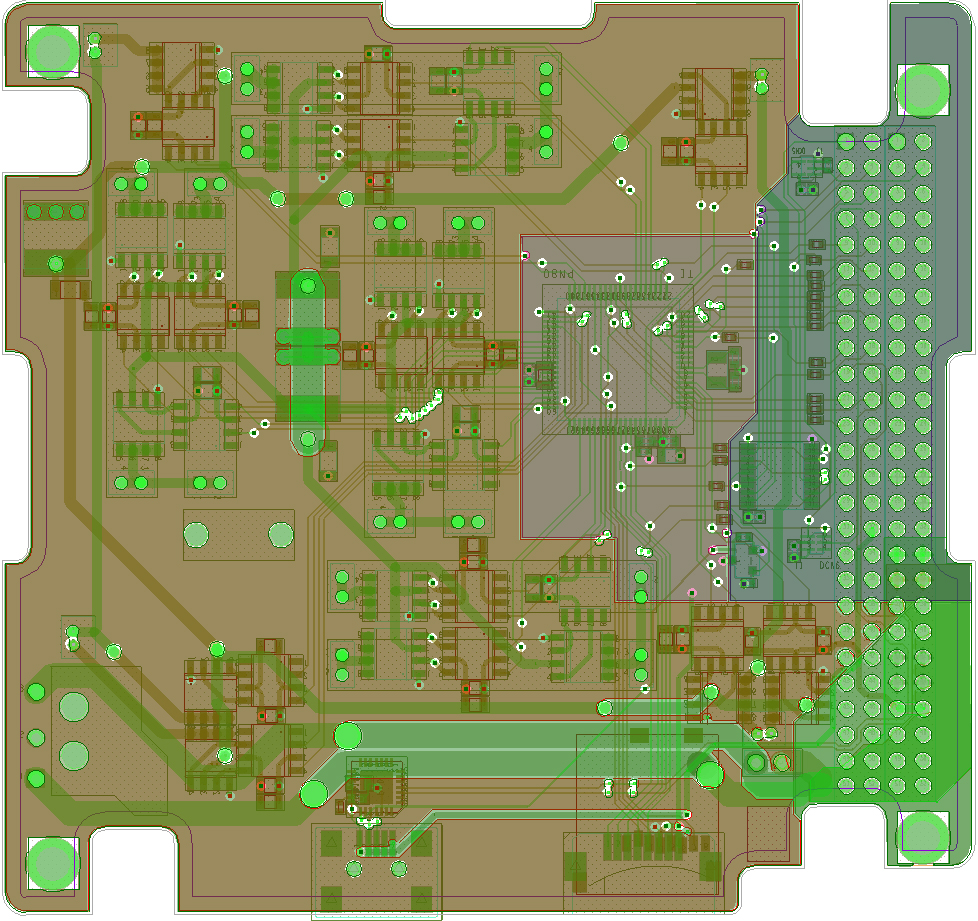
\includegraphics[width=\textwidth]{board-design}
    \caption{Board Layout for the CubeSat \acs*{ACDS} system}
    \label{fig:layout}
\end{figure}

\end{comment}

%% vim: set filetype=tex spell :

\chapter{Hardware}

\label{ch:Hardware}

\section{MSP430}

The MSP430 is at the 

\section{Data Storage}

\section{Torquers and Driving Circuit}

\subsection{Mechanical Considerations}

\section{Board Layout}

\begin{figure}[H]
    \centering
    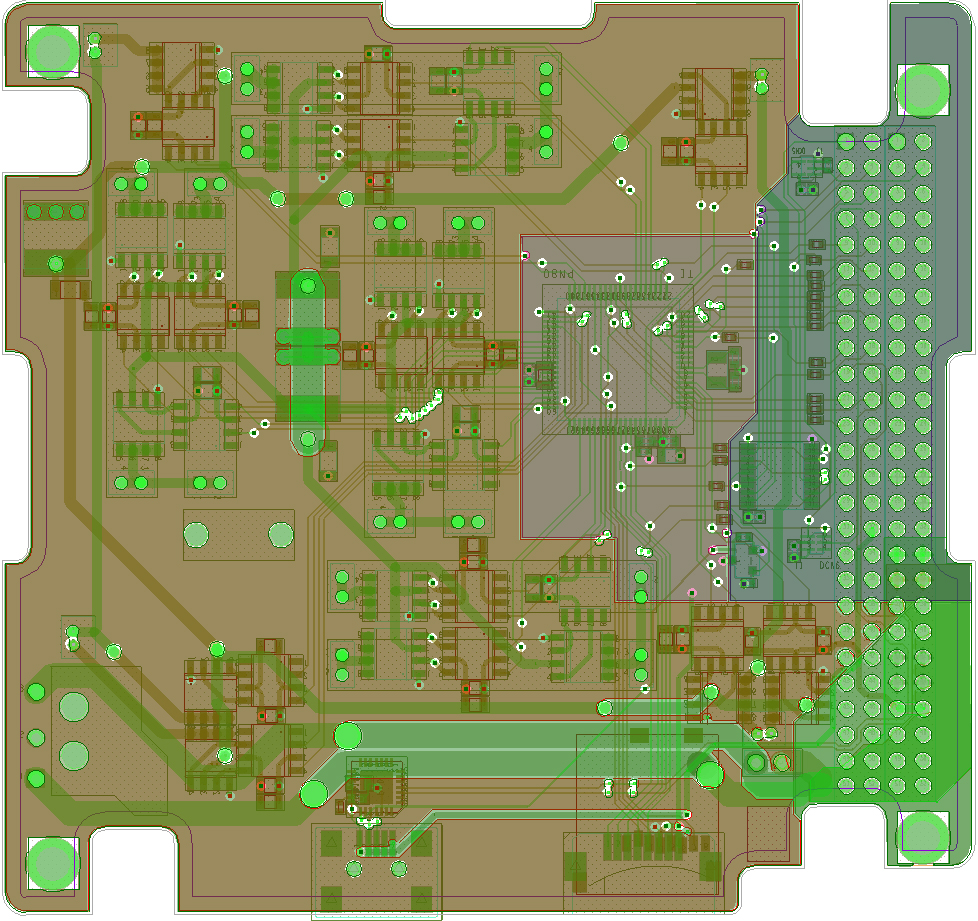
\includegraphics[width=0.8\textwidth]{board-design}
    \caption{Board Layout for the CubeSat \acs{ADCS} system}
\end{figure}

\begin{comment}

\section{Board Renderings}

\begin{figure}[H]
    \centering
    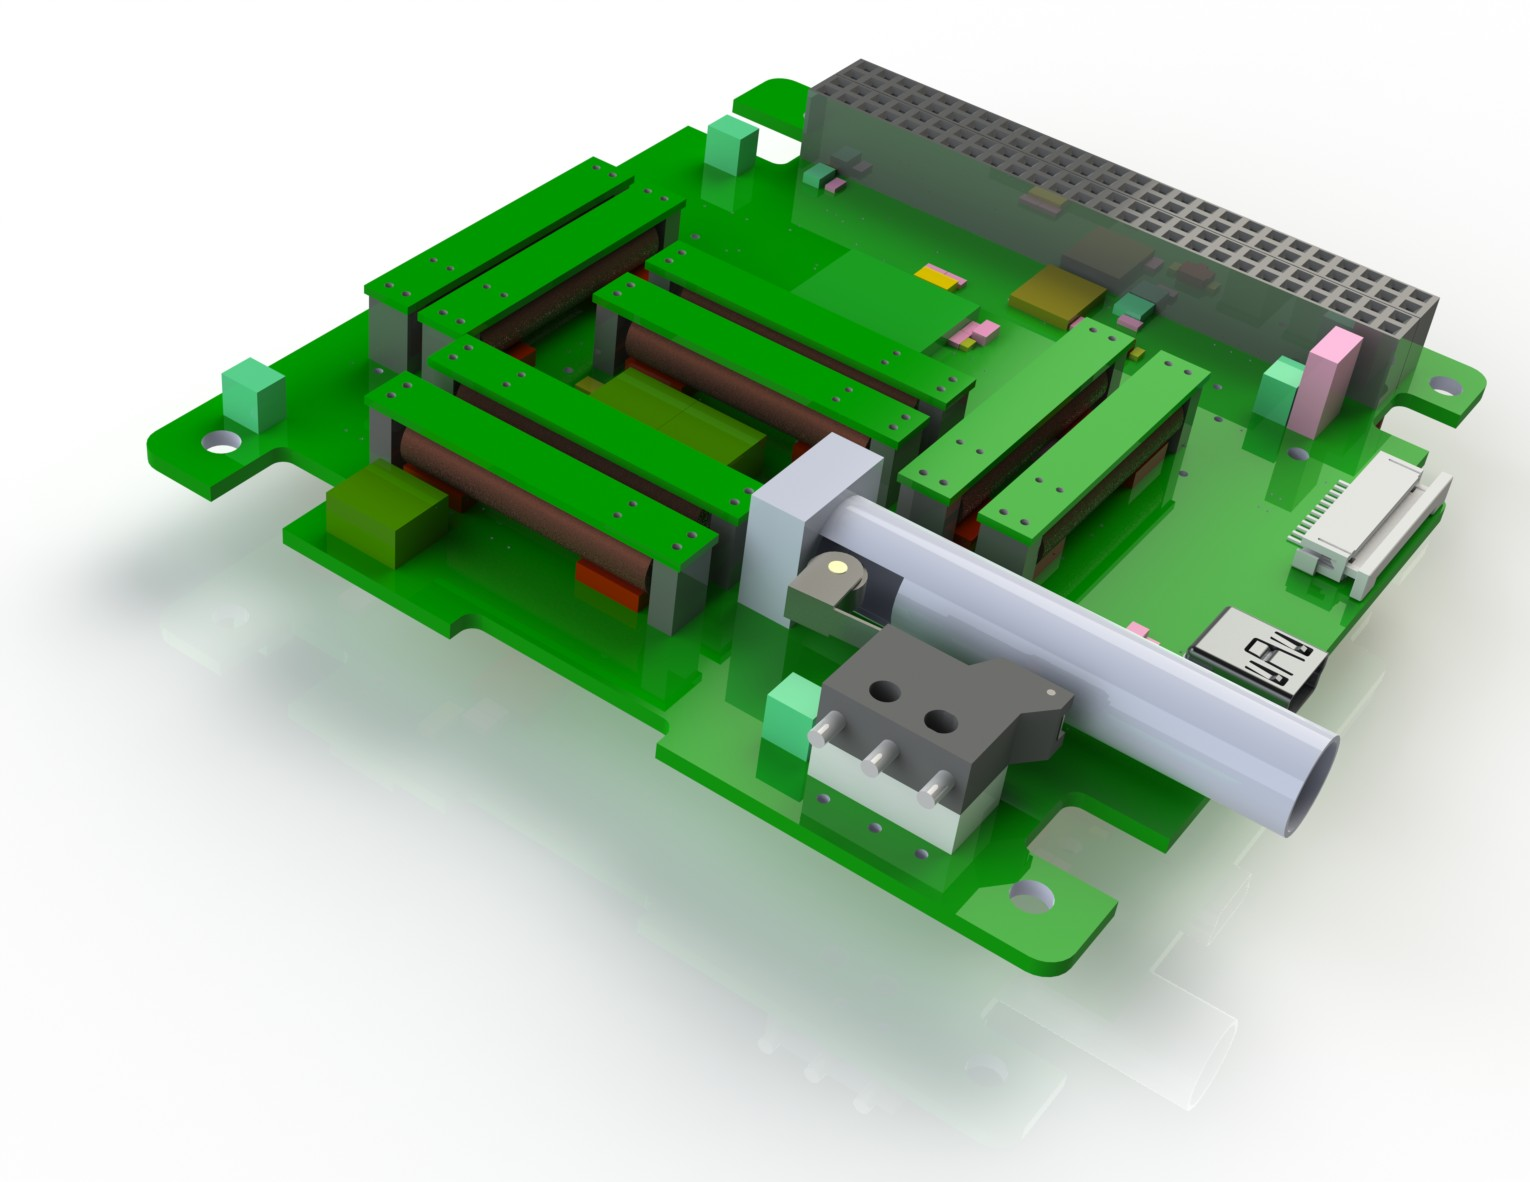
\includegraphics[width=0.8\textwidth]{board-drawing}
    \caption{3D view of the CubeSat \acs{ADCS} system}
\end{figure}

\begin{figure}[H]
    \centering
    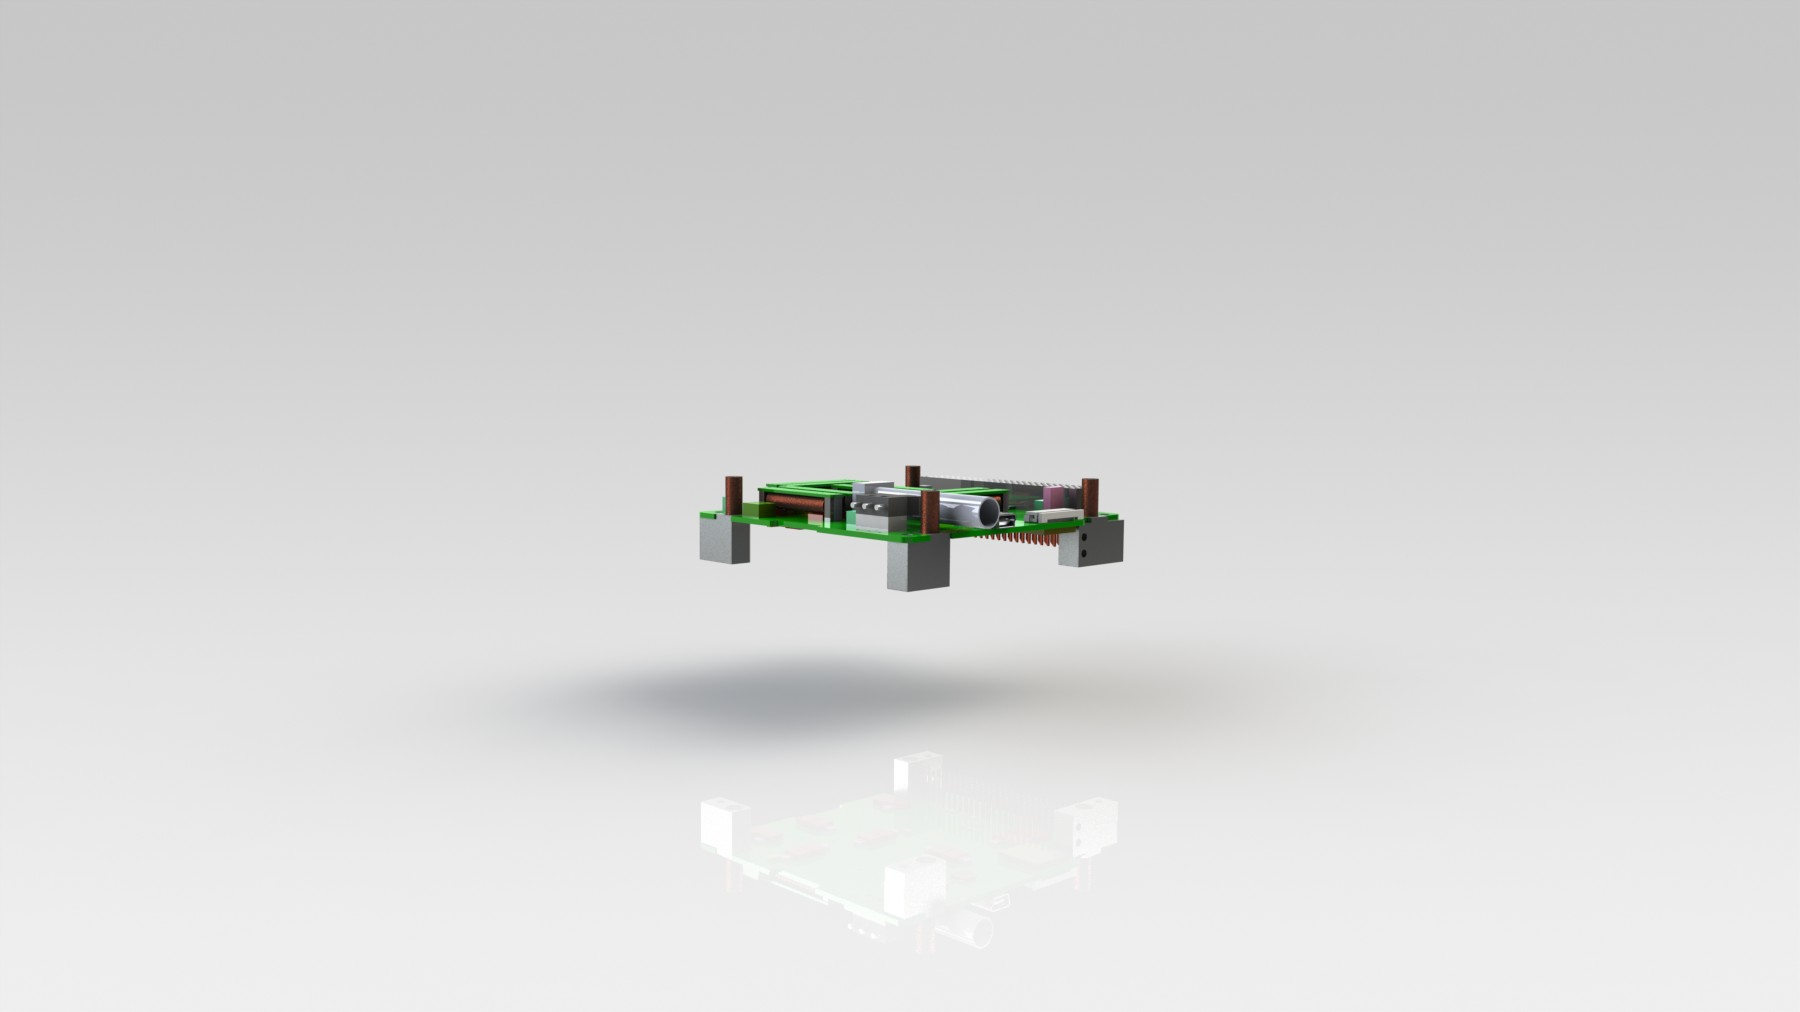
\includegraphics[width=0.8\textwidth]{board-drawing-with-standoffs}
    \caption{3D view of the CubeSat \acs{ADCS} system with Z-axis torquers}
\end{figure}

\end{comment}

% vim: filetype=tex spell

\chapter{Software}
\label{ch:Software}

The main responsibility of the \ac{ACDS} software is to determine which torquer to flip each time step. The \ac{ACDS} also needs to keep track of \enquote{house keeping} information, sensor readings, torquer states and internal control system states so that the performance of the algorithm can be tracked on the ground. 

\section{Overview}

In order to determine which torquer to flip the \ac{ACDS} needs sensor inputs. The sensors are read by the \ac{LEDL} board and forwarded to the \ac{ACDS} using the \ac{ARC}bus. The \ac{ACDS} needs to communicate with the \ac{COMM} board to respond to ground station commands and downlink housekeeping data.

\begin{figure}[H]
    \centering
    %separator for parallel lines
    \def\linesep{6}
    \begin{tikzpicture}[node distance = 1cm, auto]
        % Place nodes
        \node [block,minimum height=8cm]            (AB) {\acs{ARC}bus interface};

        \node [block,node distance=4cm,left=of AB]  (LEDL) {\acs{LEDL}};
        \node [block,left=of AB,yshift=-3cm]        (CDH) {\acs{CDH}};
        \node [block,left=of CDH]                   (COM) {\acs{COMM}};

        \node [bigblock,node distance=4cm,right=of AB,minimum height=5cm,yshift=1.5cm] (core) {\acs{ACDS} software};
        \node [bigblock,node distance=1cm,below=of core,minimum height=2cm] (HC) {House Keeping};


        \path [flow] (AB.58) -- node  {Sensor Data} (core.170);
        \path [flow] (core.190) -- node {Sensor Commands} (AB.48);

        \path [flow] (AB.00) -- node {Ground Station} node [below]{Commands} (core.226);

        \path [flow] (core) -- (HC);
        \path [flow] ([yshift= \linesep]AB.290)  -- node [above]{Data Log Query} ([yshift= \linesep]HC.west);
        \path [flow] ([yshift=-\linesep]HC.west) -- node [below]{Recalled Data} ([yshift=-\linesep]AB.290);

        \path [flow] ([yshift= \linesep]COM.east) -- ([yshift= \linesep]CDH.west);
        \path [flow] ([yshift=-\linesep]CDH.west) -- ([yshift=-\linesep]COM.east);

        \path [flow] ([yshift= \linesep]CDH.east) -- ([yshift= \linesep]AB.250);
        \path [flow] ([yshift=-\linesep]AB.250)   -- ([yshift=-\linesep]CDH.east);

        \path [flow] ([yshift=-\linesep]LEDL.east) -- node [below]{Sensor Data}     ([yshift=-\linesep]AB.west);
        \path [flow] ([yshift= \linesep]AB.west)   -- node [above]{Sensor Commands} ([yshift= \linesep]LEDL.east);


    \end{tikzpicture}
    \caption{\acs*{ACDS} software overview}
\end{figure}

\section{System Operations Overview}

The \ac{ACDS} starts running after the separation switch is switched and the power system applies power to all systems. Before starting any operations the \ac{ACDS} waits for the on command from the \ac{CDH} board. After the \ac{ACDS} board receives the on command the \ac{ACDS} sends a command to the \ac{LEDL} board to tell it to start taking sensor data. Once sensor data is received the \ac{ACDS} starts to run the detumble algorithm.


\subsection{Ground Station Commands}

The ground station can force the \ac{ACDS} into any mode and ether let it go with the normal flow or stay in a particular mode. This allows for recovery in case the system does not function as expected.

\subsection{Rotation Runaway}

If the gyros detect that the satellite is rotating too fast then they will automatically send the \ac{ACDS} into a safe mode where the \ac{ACDS} does not run. It is possible that the \ac{ACDS} could get into a situation where the algorithm speeds up the rotation instead of slowing it down. In this situation the best thing to do is for the \ac{ACDS} to stop and wait for further intervention from the ground.

\section{Incoming Commands\textbackslash Info}

The \ac{ACDS} must respond to incoming commands that change its operation mode or uplink data. Because the \ac{ACDS} is an experimental system, it may run into unexpected problems. By uplinking commands some of the possible problems can be fixed in flight. 

\begin{comment}
\begin{itemize}
    \item Ground Station Commands
        \begin{itemize}
            \item Uplink Orbit Data
            \item Stop \ac{ACDS}
            \item Force Mode
        \end{itemize}
    \item Sensor Data
\end{itemize}
\end{comment}

\section{Algorithm Software}

\Cref{fig:swblock} shows the software block diagram for the \ac{ACDS} algorithm. Field measurements from the magnetometer are calibrated using the current torquer state and the compensation data. The B-dot algorithm uses the compensated data to calculate the dipole moments that should be generated. The dipole moments are then quantized based on \cref{fig:lpmtq-flt}. The torquers to flip are chosen based current knowledge of torquer stated as well as the desired torque. The torquer feedback checks to make sure that the torquer flip happened. The torquer status is tracked by reading the torquer feedback and by knowing which torquers were flipped.

\begin{figure}[H]
    \centering
    \begin{tikzpicture}[node distance = 0.5cm, auto]
    % Place nodes
    \node [block] (field) {Magnetic Field Measurements};
    \node [block,right=of field] (cal) {Torquer offset correction};
    \node [block, right=of cal] (alg) { $C {\dot{\vect{B}}}$ };
    \node [block, right=of alg] (q) {Torque Quantization};
    \node [block, right=of q] (choose) {Choose Torquers to fire};
    \node [block,node distance=0.7cm, right=of choose] (fire) {Fire Torquers};
    \node [block, below=of choose] (mem) {Torquer Status Tracking};
    \node [block,node distance=0.7cm, right=of mem] (sens) {Torquer feedback};

    %draw lines
    \path [conn] (field) -- (cal);
    \path [conn] (cal) -- (alg);
    \path [conn] (alg) -- (q);
    \path [conn] (q) -- (choose);
    \path [conn] (choose) -- (fire);

    \path [conn] (choose.east) ++(0.3cm,0) |- (mem.10);
    \path [phconn] (fire) -- (sens);

    \path [conn] (sens.190) -- (mem.350);
    \path [conn] (mem) -- (choose);
    \path [conn] (mem) -| (cal);

    \end{tikzpicture}
    \caption{Overall Software Block Diagram}
    \label{fig:swblock}
\end{figure}

\subsection{B-dot Algorithm}

\label{sec:bdot-desc}

The B-dot algorithm is used to detumble the \ac{ARC}. The B-dot algorithm uses the time derivative of the magnetic field, $\dot{\vec{B}}$, to calculate the magnetic dipole moment that the torquers should generate. This is a method that is widely used on other CubeSats \todo{Find some B-dot reference(s)} that have magnetic \ac{ACDS}. In this mode the magnetic dipole moment is simply set to a value that is proportional to the derivative of the magnetic field. The gain for the B-dot controller needs to be negative in order to stop the motion of the magnetic field. This could be done by adding a negative sign to the torque expression but, in code, it is simpler to have a negative gain.

\section{Auxiliary Software Functions}

In addition to the algorithm software the \ac{ACDS} also requires some auxiliary software to function. In order to generate the proper dipole moment the status of the torquers must be tracked in software so that the right torquer can be flipped. The torquer status also needs to be tracked so that the torquer offsets can be subtracted from the magnetometer measurements. 

\subsection{Torquer Flipping Logic}

The torquer flipping logic keeps track of the torquer status and sets the torquers to the dipole moment that is closest to the dipole moment requested by the control algorithm. The torquer flipping logic also attempts to distribute the flips somewhat evenly across the torquers in any given axis. This way if there are any degradation effects, in the torquer field or the hardware, they will be minimized. 

\subsubsection{Status Tracking}

The status of each torquer is tracked by the flipping logic. This includes flags to indicate if each torquer has been flipped and has had errors being flipped. The last four torquers that were flipped are also tracked. This is used to chose which torquer to flip.

When it is time to flip a torquer the software looks at the current torquer status to figure out which direction a torquer needs to be flipped in. Next the software looks for the torquer that can be flipped in that direction that was flipped the least recently and flips it. This way the torquer flips are distributed across the torquers in a given axis. If torquers are marked as uninitialized then they are flipped first before other torquers so that all torquers are in a known state as quickly as possible.

\subsubsection{torquer feedback}

Before and after each torquer flip the torquer feedback comparators are read. After the torquer flip is complete the feedback values are examined to determine if the torquer flipped. If the capacitor voltage was below the upper threshold before the flip then an error is flagged in the torquer status indicating that there is a problem with the capacitor. If the capacitor voltage after a flip is not below the lower threshold then there is likely a bad connection to the torquer windings. Torquers that failed to flip are flagged and not flipped in the future. It is possible that the comparator could malfunction and indicate that it is both above the upper threshold and below the lower threshold in this case a flag is set to indicate the error and the torquer is assumed to have flipped as normal.

\subsection{Torquer Compensation}

Because the geometry of the system should not change in flight, the field offset seen by each magnetometer depends on the combination of torquer states. By taking measurements in the Helmholtz cage these offsets can be calculated and eliminated during flight in order to measure Earth's magnetic field.

\subsubsection{Compensation Data Set}

\label{sec:comp-dat-set}

There are a total of 12 \acp{LPMT} on the \ac{ACDS}. Each \ac{LPMT} has two states which results in a total of 4096 possible states. If the offset for each state uses four bytes this results in a data set that is 16kB. The field produced at each state however, is the sum of the field contributions of all of the torquers. The dataset can be reduced by doing three separate calibration, one for the set of torquers in each axis. The calibrations are then combined to get a calibration set where one offset is chosen for each axis and added together to get the full offset this reduces the number of states to $3*16 + 1 = 49$ which is only about 200 bytes of data, much reduced from using all possible states.

\subsubsection{Compensation Routine}

\label{sec:tq-comp}

To calculate the compensation values for the torquers the calibration procedure described in \cref{sec:magcal} is run for each combination of torquer states. The results of the compensation is $C_1$, $C_2$, $C_4$ and $ C_5$ which are the same calibration constants computed with the magnetometer calibration routine. In addition there is one common pair of offsets and then 3 sets of 16 offsets for each set of torquers. The total offset value for a given torquer state is the sum of the common offset value and an offset determined by the state of the torquers in the X, Y and Z axes.

\subsection{Data Logging}

During \ac{ACDS} operations data is collected during flight. This data is stored in nonvolatile memory and can be recalled and transmitted to the ground in order to evaluate the \ac{ACDS} system performance. The data that is recorded is shown in \cref{tab:logdat}

\begin{comment}
\begin{itemize}
    \item magnetometer and gyro readings
    \item torquer status
    \item mode
    \item algorithm intermediate results
    \item torquers flipped
    \item torquer feedback
    \item Kalman filter status
    \item Kalman filter internal variables
    \item Kalman filter state
    \item \todo[inline]{More?}
\end{itemize}
\end{comment}

\begin{table}[H]
    \centering
    \caption{\ac{ACDS} operations data format}
    \label{tab:logdat}
    \begin{tabular}{|l|c|c|}
        \hline
        Data&size (bits)&Format\\
        \hline
        mode&2&unsigned integer\\
        \hline
        Time Stamp&32&unsigned integer\\
        \hline
        torquer status&48&flags\\
        \hline
        magnetometer readings&48&unsigned integer (one per axis)\\
        \hline
        gyro readings&36&unsigned integers (one per axis)\\
        \hline
        algorithm intermediate results&TBD&\\
        \hline
        torquers flipped&48&unsigned integer (one per axis)\\
        \hline
        torquer feedback&12&flags\\
        \hline
        Kalman filter status&TBD&\\
        \hline
        Kalman filter internal variables&TBD&\\
        \hline
        \multicolumn{1}{|r|}{\bfseries Total :}&TBD&\\
        \hline
    \end{tabular}
    \todo[inline]{Resolve DBD's}
\end{table}

\subsection{On Board data processing}

Because the downlink data speed is limited, it is necessary to reduce the data that needs to be downlinked. One way to do this is to do some level of on board processing to reduce the data before it is downlinked. For the \ac{ACDS} system this will most likely take the form of returning only the desired data from the recorded data set or returning min/max values from within a data set. 

\subsection{Beacon Data}

The beacon data is transmitted at a fixed rate and provides information about the present state of the satellite. The beacon data could be the only data that is available to diagnose the system. The beacon data must contain enough data to be useful but not so much data that the beacon packets are too big. The beacon data should include raw sensor information as well as information on torquer status. The beacon data from the \ac{ACDS} is shown in \cref{tab:beacondat}

\begin{table}[H]
    \centering
    \caption{Beacon Data format}
    \label{tab:beacondat}
    \begin{tabular}{|l|c|c|}
        \hline
        Data&size (bytes)&Format\\
        \hline
        current magnetometer readings&6&signed integers (one per axis)\\
        \hline
        Mode&1&unsigned integer\\
        \hline
        current torquer status&3&flags\\
        \hline
        number of torquer flips so far & 6 & unsigned integers (one per axis)\\
        \hline
        Kalman filter attitude&8&integer quaternion\\
        \hline
        Kalman filter rates&6&integer vector\\
        \hline
        \multicolumn{1}{|r|}{\bfseries Total :}&30&\\
        \hline
    \end{tabular}
\end{table}


% vim: set filetype=tex spell :

\chapter{Verification}

\label{ch:Verification}

The \ac{ACDS} consists of experimental hardware controlled by experimental software and as such requires a significant amount of verification to make sure everything functions on orbit.

\section{Sensor Verification}

\subsection{Magnetomitor Verification}

The magnetomitor verification is done using the Hemholtz cage 

\subsection{Gyro Verification}

\subsection{Feedback Verification}

To test the torquer feedback 

\section{\acl{ADS} Verification}

\section{Torquer Verification}

\subsection{Driver Verification}

To test the torquer drivers 


\section{Software Verification}

\section{System Verification}

Testing of torquer calibration

Magnetic interference from currents


% vim: filetype=tex spell

\chapter{Conclusion and Future work}

\section{Conclusion}

The goal of this thesis was to make a working prototype of an \ac{ACDS} using \acp{LPMT}, as described by Donald Mentch in \cite{Mentch11}. For this thesis flight hardware has been built with software to detumble the satellite. The alignment phase, using bias windows to establish and maintain desired alignment, was not implemented primarily because the rotation rates proved more complex to calculate than originally described in \cite{Mentch11}. In addition the orbit in \cite{Mentch11} was circular and for the \ac{ARC}1 mission the orbit will be elliptical.

In a circular orbit the angular velocity required to remain nadir pointing is constant throughout the orbit. In an elliptical orbit the angular velocity to remain nadir pointing is not constant throughout the orbit. The changing angular velocity presents a problem because the algorithm in \cite{Mentch11} works by setting the angular velocity of the satellite to be constant. 

A large part of the work for this thesis was focused on the torquer compensation. Torquer compensation is needed so that the Earth's magnetic field can be measured using magnetometers that are not separated from the torquers. It was suggested that torquer compensation was possible but it was not mentioned in \cite{Mentch11}. Software has been written to interface with the \ac{LEDL} board to read magnetometer data and compensate for the torquer field. The torquer compensation has been tested and found to accurately measure the external magnetic field well enough to compute the attitude to within \textpm{}5\textdegree.

\section{Future Work}

\label{sec:future-work}

The system built for this thesis does not fully implement everything described in \cite{Mentch11}. The main shortcomings of the described system is the software. The hardware is essentially the same as described in \cite{Mentch11} except for the torquer sizing.

The torquers as described in \cite{Mentch11} are not feasible. The torquer flips in \cref{fig:satWV} showed about a \textpm{}0.5\% variation across multiple flips. The vernier torquers described in \cite{Mentch11} were $\sfrac{1}{200}^{\mathrm{th}}$, or 0.5\%, the strength of the primary torquers. The result is that a set of primary torquers that is set to produce zero torque could produce the same amount of torque as a pair of vernier torquers. The solution used in this thesis was to not use the vernier torquers and fill the empty slots with primary torquers. This could be improved upon if a torquer core could be made with approximately 10\% the dipole moment of the alnico torquers. 

The rotation rate determination algorithm was found to be a much more complex problem than described in \cite{Mentch11} which suggested that rotation rates could be determined directly from magnetic field measurements. Upon further investigation it was found that this was not feasible for the alignment phase. As an alternative the rotation rates can be determined from the magnetic field using a Kalman filter. The Kalman filter brings an additional level of complexity that the original system attempted to avoid. 

The Kalman filter uses a magnetic field model for attitude determination. The magnetic field model uses the location of the satellite to calculate the expected local magnetic field in the orbital reference frame. This requires that the position of the satellite be known for the Kalman filter to work. The location will be calculated by uplinking the orbital parameters of the satellite and using an orbit propagator to calculate position as the satellite moves through its orbit.

The bias windows were originally supposed to be determined using the magnetic field to estimate the latitude. With the Kalman filter the location can be directly determined using the orbit propagator so there is no need for latitude determination from the Earth's magnetic field.

\subsection{New Concept of Operations}

The algorithm shown in \cref{fig:swblock} with additions is shown in \cref{fig:swblock-future}. The orbital parameters are used to determine the bias window and to determine the local magnetic field direction. The Kalman filter is used to output rates to the torque algorithm. The bias window is used by the torque algorithm to determine when and how to bias the torquers.

\begin{figure}[H]
    \centering
    \begin{tikzpicture}[node distance = 0.5cm, auto]
    % Place nodes
    \node [block] (field) {Magnetic Field Measurements};
    \node [block,right=of field] (cal) {Torquer offset correction};
    \node [block,node distance=0.7cm,right=of cal] (alg) {Torque algorithm};
    \node [block, right=of alg] (q) {Torque Quantization};
    \node [block,above=of cal] (igrf) {Magnetic field model};
    \node [block,node distance=0.7cm,right=of igrf] (rates) {Kalman Filter};
    \node [block,left=of igrf] (pos) {Orbit Propagator};
    \node [block, above=of q] (win) {Bias Window Determination};
    \node [block, right=of q] (choose) {Choose Torquers to fire};
    \node [block,node distance=0.7cm, right=of choose] (fire) {Fire Torquers};
    \node [block, below=of choose] (mem) {Torquer Status Tracking};
    \node [block,node distance=0.86cm, below=of fire] (sens) {Torquer feedback};

    %draw lines
    \path [conn] (field) -- (cal);
    \path [conn] (cal.east) -- ++(0.3cm,0) |- (rates.190);
    \path [conn] (cal) -- (alg);
    \path [conn] (rates) -- (alg);
    \path [conn] (win) -- (alg);
    \path [conn] (alg) -- (q);
    \path [conn] (q) -- (choose);
    \path [conn] (choose) -- (fire);

    \path [conn] (choose.east) -- ++(0.3cm,0) |- (mem.10);
    \path [phconn] (fire) -- (sens);

    \path [conn] (sens.west) -- ++(-0.3cm,0) |- (mem);
    \path [conn] (mem) -- (choose);
    \path [conn] (mem) -| (cal);

    \path [conn] (pos) -- (igrf);
    \path [conn] (igrf.east) -- ++(0.3cm,0) |- (rates.west);

    \path [conn] (pos) |- ([yshift=0.3cm]win.north) -- (win);

    \end{tikzpicture}
    \caption{Overall Software Block Diagram}
    \label{fig:swblock-future}
\end{figure}

The torque algorithm varies depending on the current mode. In mode 1 the Kalman filter and bias window determination are not used and the algorithm is the one showin in \cref{fig:swblock}. In modes 2 and 3 the algorithms shown in \cref{fig:mode2,fig:mode3} are used.

\subsubsection{Mode 2}

\Cref{fig:mode2} shows the Mode 2 torque algorithm block diagram. Torque is calculated the same way as in Mode 1 but this time a bias is added depending on which region of the orbit the satellite is in. The bias tends to cause the satellite to rotate. This causes the algorithm to cancel out the bias. This is prevented by preventing the resulting dipole moment from being in the opposite direction as the bias. Outside of the bias regions the torquers are set to produce no torque.

\begin{figure}[H]
    \centering
    \begin{tikzpicture}[node distance = 0.5cm, auto]
    % Place nodes
    \node [input] (field) {Magnetic Field};
    \node [block, right=of field] (alg) { $k \frac{\vect{\omega}_{err} \cross \vect{B}}{\vect{B} \cdot \vect{B}}$ };
    \node [input, right=of alg] (rates) {Rotation Rates};
    \node [oppr,node distance=1cm,below=of alg] (sum) {+};
    \node [block,node distance=1.2cm,left=of sum] (bias) {Mode 2 bias table};
    \node [input,left=of bias] (win) {Bias Window};
    \node [block,node distance=1cm,below=of sum] (fix) {Bias Fix};
    \node [block,below=of fix] (coast) {Coast?};
    \node [point, below=of coast] (out) {};

    %draw lines
    \path [conn] (field) -- (alg);
    \path [conn] (rates) -- (alg);
    \path [conn] (alg) -- (sum);
    \path [conn] (win) -- (bias);
    \path [conn] (bias) -- (sum);
    \path [conn] (sum) -- (fix);
    \path [conn] (fix) -- (coast);
    \path [conn] (win) |- (coast);
    \path [conn] (coast) -- (out);
    \path [conn] (bias) |- (fix);

    \end{tikzpicture}
    \caption{Mode 2 Torque Algorithm Block Diagram}
    \label{fig:mode2}
\end{figure}

\subsubsection{Mode 3}

\Cref{fig:mode3} shows the Mode 3 torque algorithm block diagram. This is similar to Mode 2 except only the north pole bias window is used and outside the bias window torque is generated to slow rotation rates.

\begin{figure}[H]
    \centering
    \begin{tikzpicture}[node distance = 0.5cm, auto]
    % Place nodes
    \node [input] (field) {Magnetic Field};
    \node [block, right=of field] (alg) { $k {\frac{\vect{\omega}_{err} \cross \vect{B}}{\vect{B} \cdot \vect{B}}}$ };
    \node [input, right=of alg] (rates) {Rotation Rates};
    \node [oppr,node distance=1cm,below=of alg] (sum) {+};
    \node [block,node distance=1.2cm,left=of sum] (bias) {Mode 3 bias table};
    \node [input,left=of bias] (win) {Bias Window};
    \node [block,node distance=1cm,below=of sum] (fix) {Bias Fix};
    \node [point, below=of fix] (out) {};

    %draw lines
    \path [conn] (field) -- (alg);
    \path [conn] (rates) -- (alg);
    \path [conn] (alg) -- (sum);
    \path [conn] (win) -- (bias);
    \path [conn] (bias) -- (sum);
    \path [conn] (sum) -- (fix);
    \path [conn] (fix) -- (out);
    \path [conn] (bias) |- (fix);


    \end{tikzpicture}
    \caption{Mode 3 Torque Algorithm Block Diagram}
    \label{fig:mode3}
\end{figure}

\subsection{Alternate operations}

The original system presented in \cite{Mentch11} used the biasing scheme to get the satellite into the correct attitude without ever knowing the attitude. The Kalman filter proposed for rate determination must compute attitude in order to compute the rotation rates. Because the attitude is known a more traditional attitude control algorithm to be used. Using a more traditional algorithm will allow the \ac{ACDS} to function in orbits that are elliptical. 



%% vim: filetype=tex

\chapter{Torquer Drive Circuit}

The energy to flip the torquers is stored in a capacitor that is slowly charged from the power supply and discharged quickly into a torque coil. There are three capacitors, one for each axis. 

\section{Capicitor Charging}

Figure \cref{fig:cap-chg} shows the charging circuit. The resistor limits the current from the power supply to a maximum of ?? mA. A switch is shown instead of the H-bridge for simplicity.

\section{Rational}

A resistor was chosen for the charging circuit because it is simple and robust. The main drawback of the design is that it is about 50\% efficient. The capacitor voltage also depends on the supply voltage which will vary with battery discharge depth. 

\section{H-Bridge}

The H-bridge allows current to be driven in both directions through the torquer coils. 



%% vim: set filetype=tex :
\chapter{\acs{LPMT} Algorythm}

The simulations in \cite{mench11} include the algorythm used for the \ac{ACDS}. The \ac{LPMT} algorythms had to be ported form the matlab code contained in the simulation to C code running on a microcontroler. 



\clearpage

\bibliographystyle{IEEEtranN}
\phantomsection
\bibliography{references}

%\appendix

\end{document}
